\documentclass{beamer}
\usepackage{color}
\usetheme{Pittsburgh}
\usecolortheme{whale}

\usepackage{amsmath,amsthm,amssymb}
\usepackage{graphicx}
\usepackage{booktabs}  
\usepackage[utf8]{vietnam}
\usepackage{subcaption} %subfigure
\usepackage{listings}
\usepackage[numbers]{natbib}
\usepackage{enumitem}
\usepackage{graphicx}
\usepackage{subcaption}
\usepackage{url}
\usepackage{hyperref}
\usepackage{algorithm}
\usepackage{algpseudocode}
\usepackage{pifont}
\usepackage{subcaption} %subfigure
\usepackage{cases} 
\usepackage{scrextend}

\newsavebox{\authbox}
\sbox{\authbox}{%
\centering
\begin{minipage}{0.45\linewidth}
\centering\normalsize
Người thực hiện \par
Phan Quang Khánh
\end{minipage}
\hfill
\begin{minipage}{0.45\linewidth}
\centering\normalsize
Giảng viên hướng dẫn \par
TS. Huỳnh Thế Đăng
\end{minipage}
}
	
\title{Exploiting reinforcement learning to find optimal strategy in dynamic maps}
\author[Phan Quang Khánh]{%
\usebox{\authbox}
}
\institute[Unimib]{Đại học Khoa học Tự nhiên}
\date{29 Tháng 8 2020}
\logo{
\includegraphics[width=1cm]{Pic/slide/logo.png}}

\begin{document}

\begin{frame}
\titlepage % Print the title page as the first slide
\end{frame}

\begin{frame}
\frametitle{}
\tableofcontents 
\end{frame}
%%%%%%%%%%%%%%%%%%%%%%%%%%%%%%%%%%%%%%%%%%%%%%%%%%%%%%%%%%%%%%%%%
\section{Giới thiệu}
%---------------------------------------------------------------%
\begin{frame}{Giới thiệu}
    \begin{figure}[ht]
        \begin{subfigure}{.48\textwidth}
          \centering
          
\includegraphics[width=.8\linewidth]{Pic/slide/alpha-go.png}
        \end{subfigure}
        \begin{subfigure}{.48\textwidth}
          \centering
          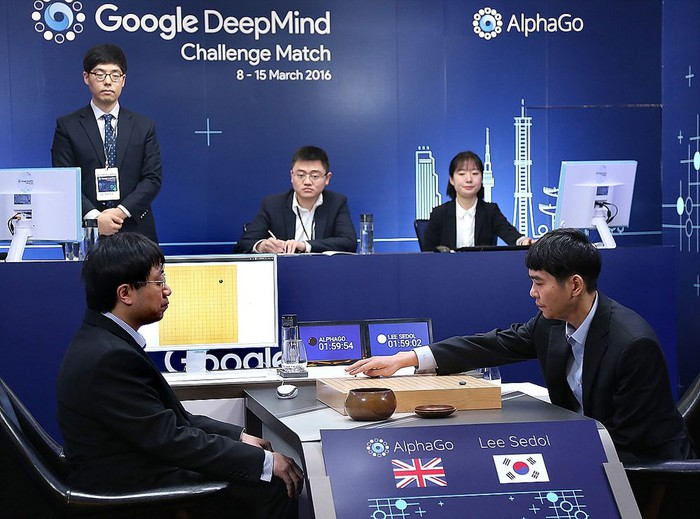
\includegraphics[width=.8\linewidth]{Pic/slide/compete with alphago.jpg}
        \end{subfigure}
    \captionsetup{labelformat=empty}
    \label{fig:fig}
    \end{figure}
\end{frame}
%---------------------------------------------------------------%
\begin{frame}{Giới thiệu}
\begin{figure}
    \centering
    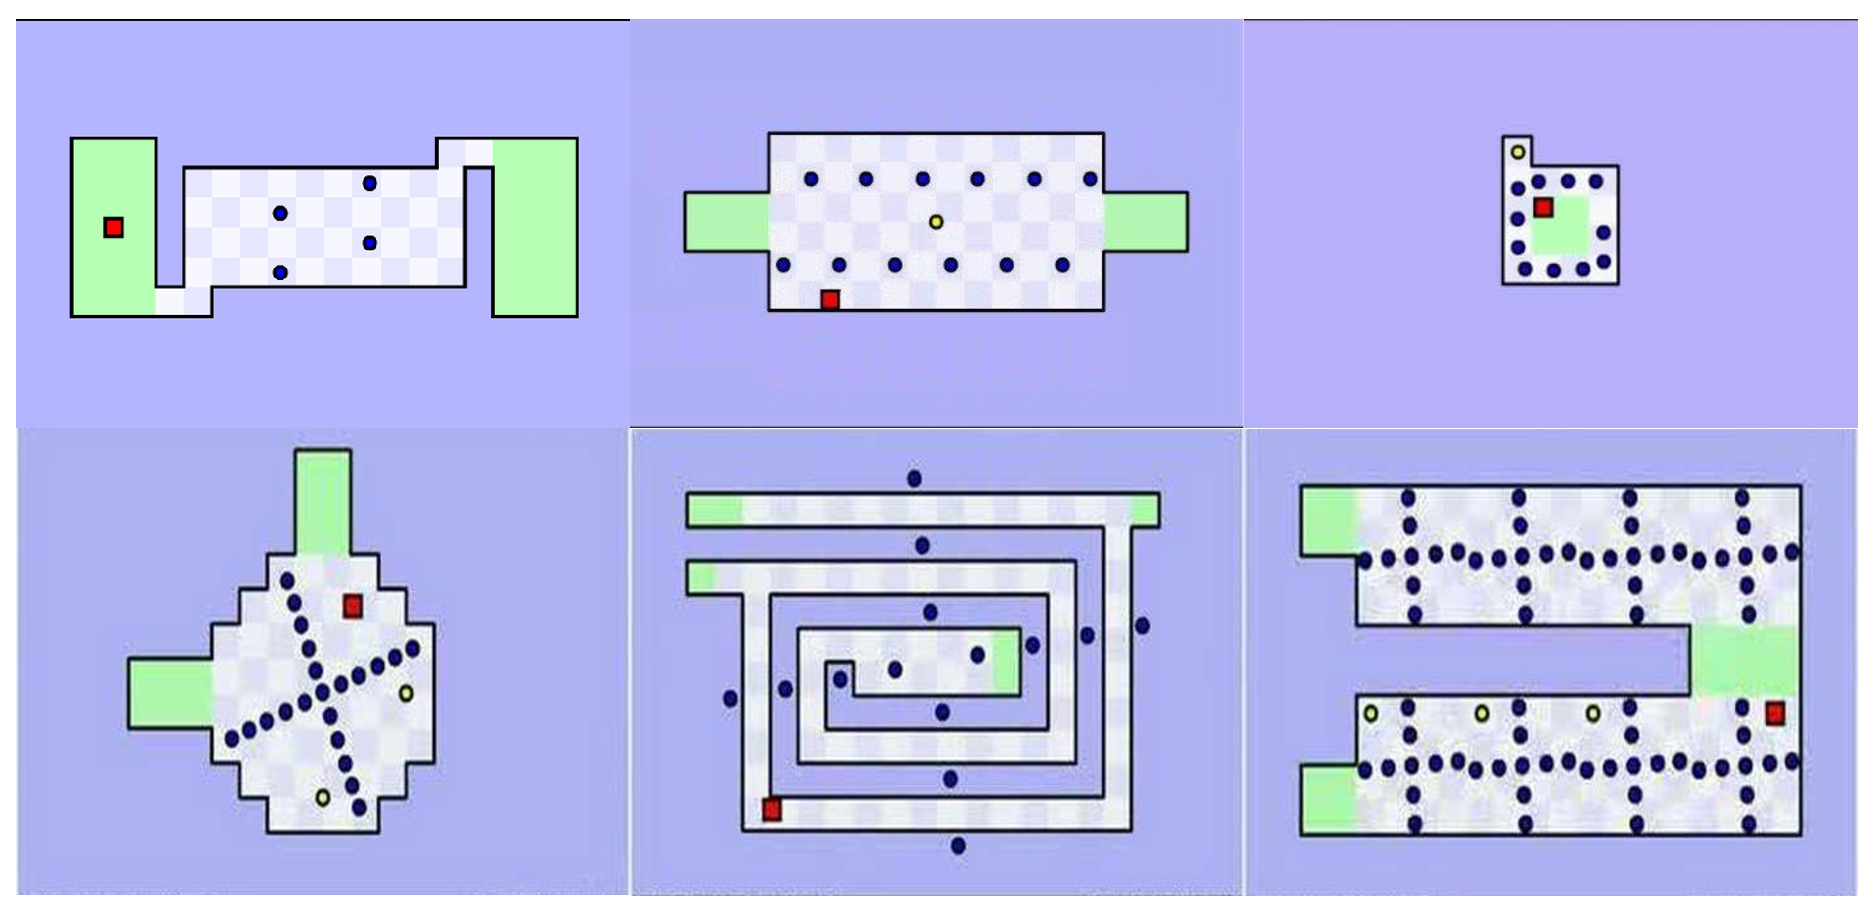
\includegraphics[width=\linewidth]{Pic/slide/WHG_level.pdf}
    \captionsetup{labelformat=empty}
\end{figure}
\end{frame}
%---------------------------------------------------------------%
\begin{frame}{Giới thiệu}
\begin{figure}
    \centering
    
\includegraphics[width=\linewidth]{Pic/slide/openai-beats-dota-2-pros-elon-musk-warns-ai-risk-scarier-n-korea.jpg}
    \captionsetup{labelformat=empty}
\end{figure}
\end{frame}
%%%%%%%%%%%%%%%%%%%%%%%%%%%%%%%%%%%%%%%%%%%%%%%%%%%%%%%%%%%%%%%%%
\section{Mục đích}
\begin{frame}{Mục đích}
Tạo ra một agent đủ thông minh để chinh phục The World's Hardest Game, đồng thời tối ưu số bước agent có thể thực hiện.
\begin{figure}
	\centering
	
\includegraphics[scale=0.4]{Pic/slide/best-ai.png}
	\captionsetup{labelformat=empty}
\end{figure}
\end{frame}
%%%%%%%%%%%%%%%%%%%%%%%%%%%%%%%%%%%%%%%%%%%%%%%%%%%%%%%%%%%%%%
%---------------------------------------------------------------%
\section{Phương pháp và kết quả}
\subsection{Chuẩn bị môi trường}
\begin{frame}{Phương pháp và kết quả}
	\centering
	\huge\textbf{CHUẨN BỊ MÔI TRƯỜNG}
	\vfill
	\begin{itemize}
	    \item \small I.   Môi trường Java
	    \item \small II.  Môi trường Socket
	    \item \small III. Môi trường Python
	\end{itemize}
\end{frame}
%---------------------------------------------------------------%
\begin{frame}{Môi trường Java}
\begin{figure}
	\centering
	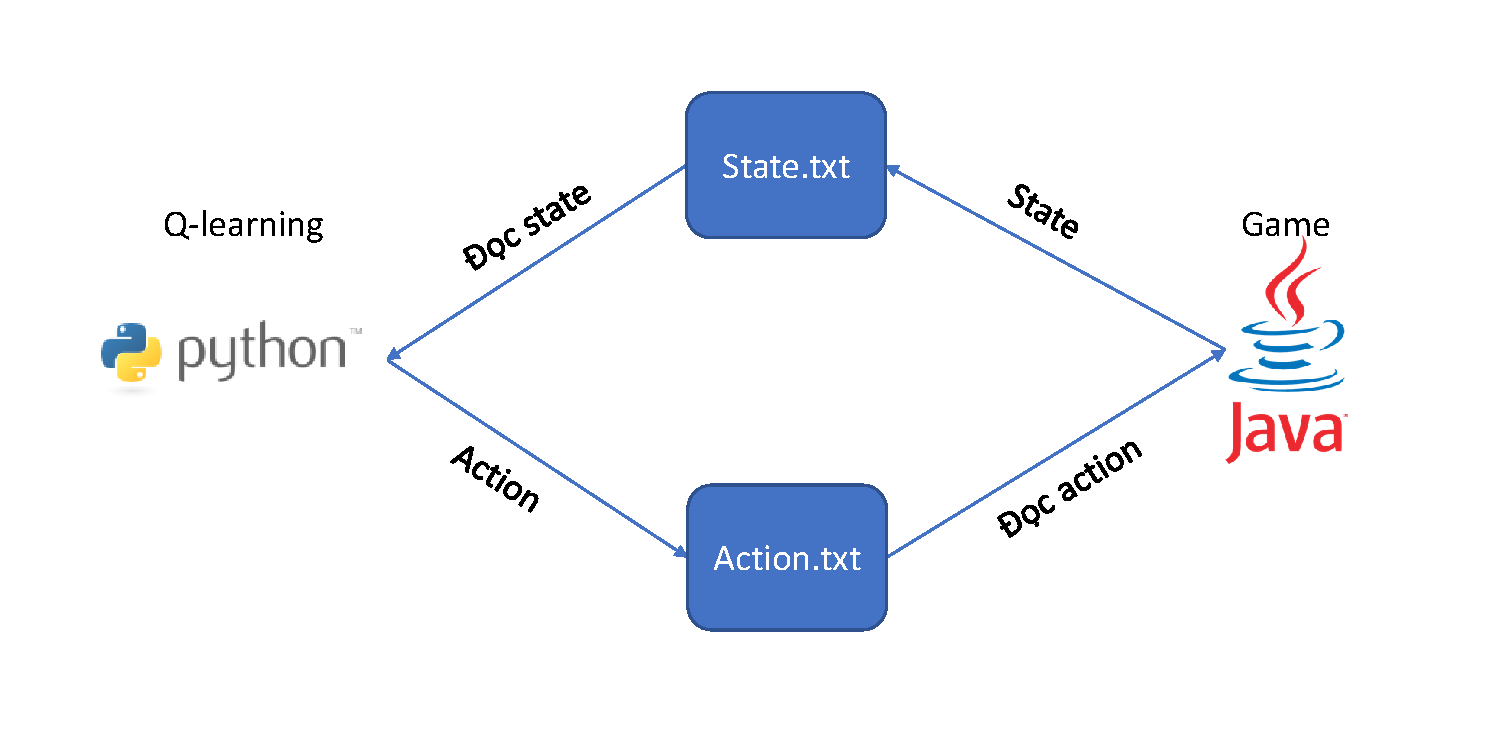
\includegraphics[scale=.4]{Pic/transfer_java_env}
	\captionsetup{labelformat=empty}
\end{figure}
\end{frame}
%---------------------------------------------------------------%
\begin{frame}{Môi trường Java}
	Huấn luyện trên môi trường java vẫn rất tốn thời gian khi chỉ thực hiện được \textbf{20 frames} trên 1 giây.
	\begin{figure}
		\centering
		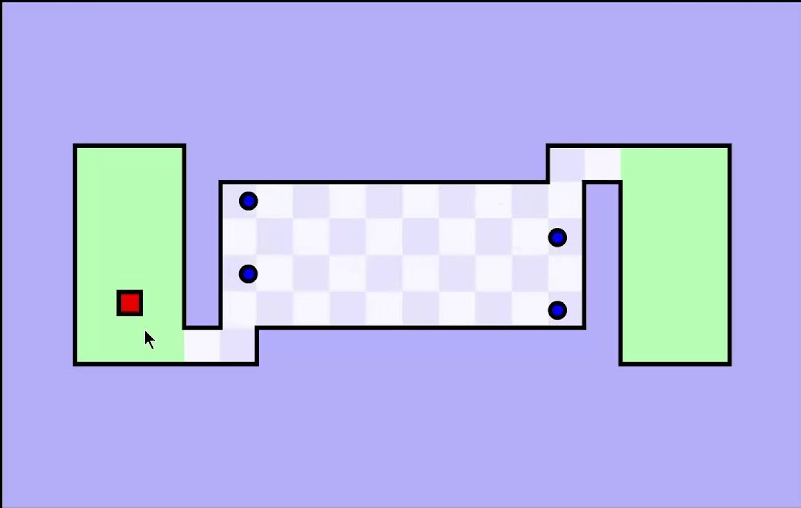
\includegraphics[scale=.3]{Pic/slide/WHG_lv1}
		\captionsetup{labelformat=empty}
	\end{figure}
\end{frame}
%---------------------------------------------------------------%
\begin{frame}{Môi trường Socket}
	Tốc độ đạt được \textbf{500 frames} trên 1 giây.
	\begin{figure}
		\centering
		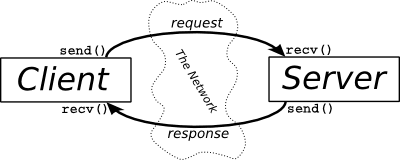
\includegraphics[scale=.5]{Pic/slide/socket-client}
		\captionsetup{labelformat=empty}
	\end{figure}
\end{frame}
%---------------------------------------------------------------%
\begin{frame}{Môi trường Socket}
	\begin{figure}
		\centering
		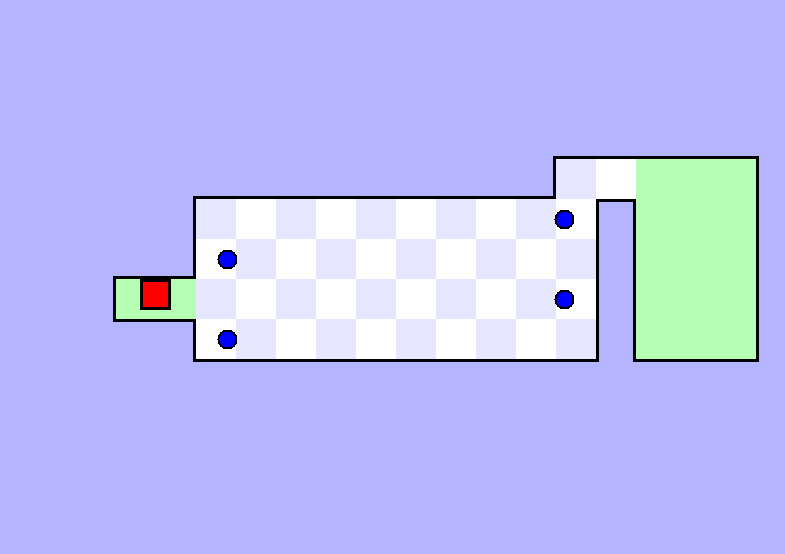
\includegraphics[scale=.3]{Pic/slide/env_NoGO}
		\captionsetup{labelformat=empty}
	\end{figure}
\end{frame}
%---------------------------------------------------------------%
\begin{frame}{Môi trường Socket}
	\begin{figure}
		\centering
		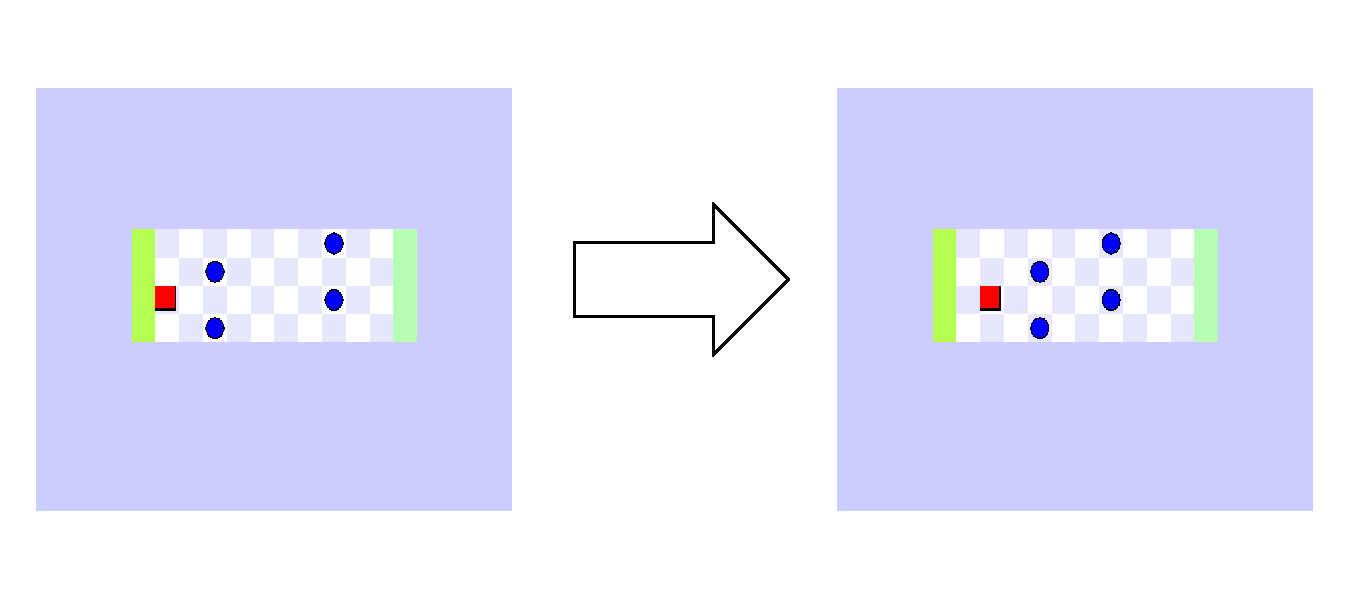
\includegraphics[scale=.5]{Pic/1_step_new_env}
		\captionsetup{labelformat=empty}
	\end{figure}
\end{frame}
%---------------------------------------------------------------%
\begin{frame}{Môi trường Python}
	\begin{figure}
		\centering
		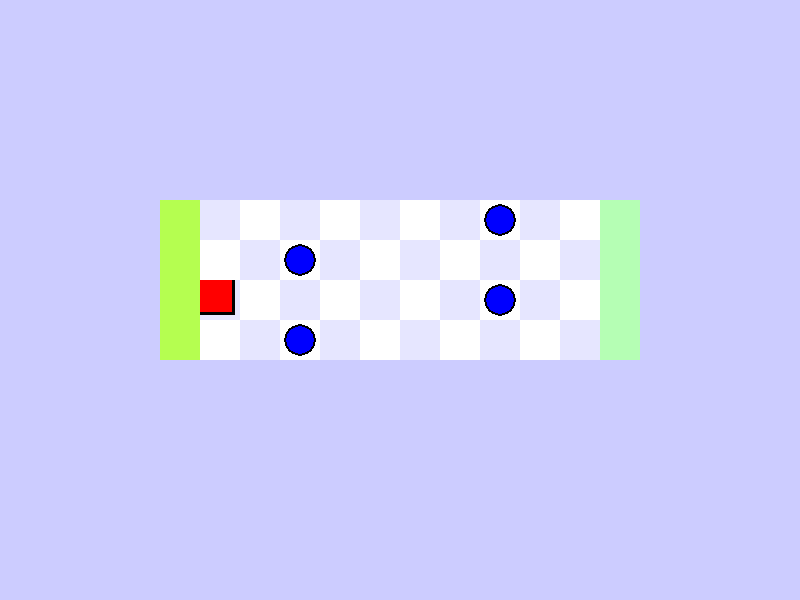
\includegraphics[scale=.3]{Pic/slide/new_env}
		\captionsetup{labelformat=empty}
	\end{figure}
\end{frame}
%---------------------------------------------------------------%
%---------------------------------------------------------------%
\subsection{Mô hình cơ sở}
\begin{frame}{Phương pháp và kết quả}
	\centering
	\huge\textbf{MÔ HÌNH CƠ SỞ}
	\vfill
	\begin{itemize}
	    \item \small I.  Điều chỉnh trạng thái
	    \item \small II. Mô hình đề xuất
	\end{itemize}
\end{frame}
%---------------------------------------------------------------%
\begin{frame}{Điều chỉnh trạng thái}
	\begin{figure}
		\centering
		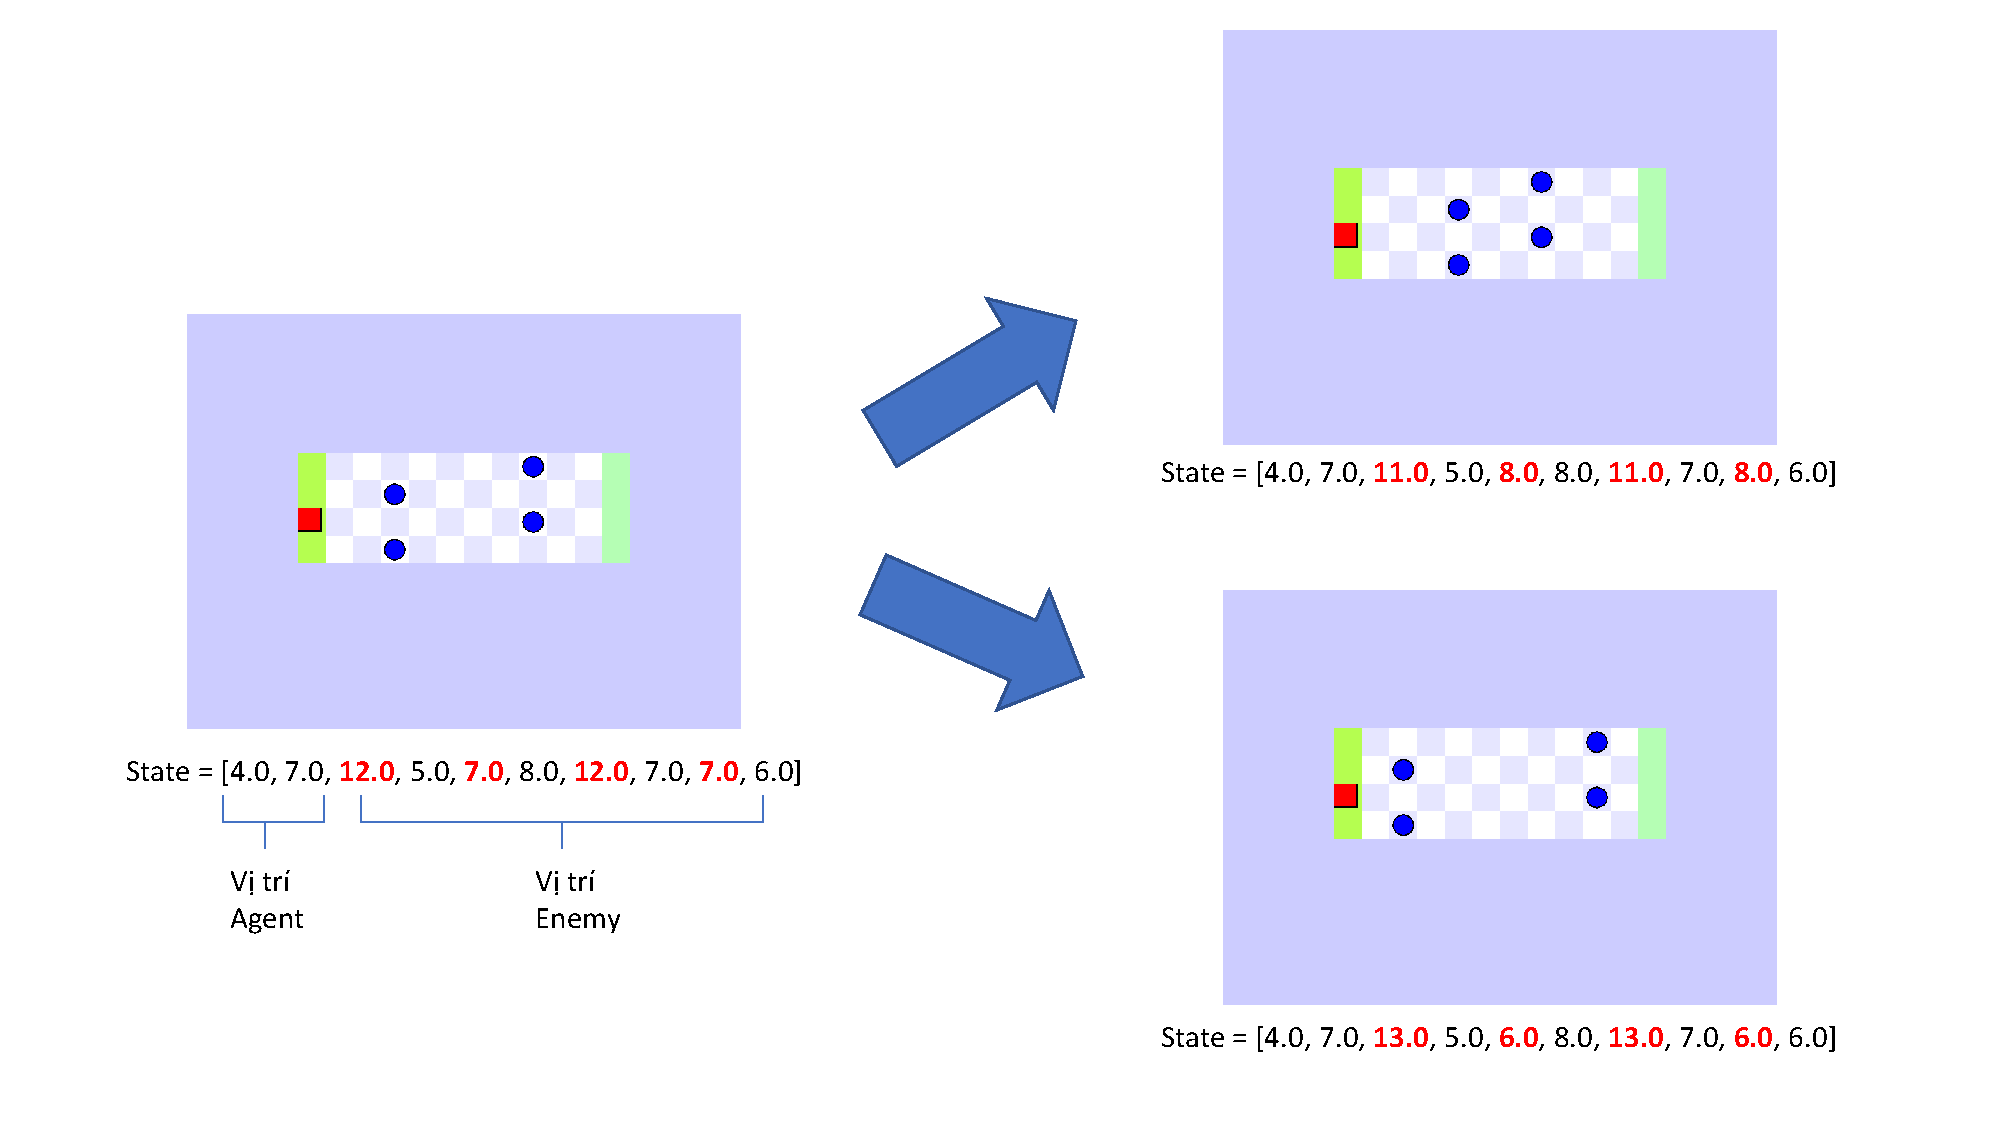
\includegraphics[scale=0.3]{Pic/conflict_enemy_position}
	\end{figure}
\end{frame}
%---------------------------------------------------------------%
\begin{frame}{Điều chỉnh trạng thái}
	\centering
	State = [4.0,7.0,\textcolor{blue}{12.0,5.0},\textcolor{cyan}{7.0,8.0},\textcolor{blue}{12.0,7.0},\textcolor{cyan}{7.0,6.0}]\\
	\hspace{1cm}
	\vfill
	State = [4.0,7.0,\textcolor{blue}{12.0,5.0},\textcolor{red}{1},\textcolor{cyan}{7.0,8.0},\textcolor{red}{0},\textcolor{blue}{12.0,7.0},\textcolor{red}{1},\textcolor{cyan}{7.0,6.0},\textcolor{red}{0}]
\end{frame}
%---------------------------------------------------------------%
\begin{frame}{Mô hình đề xuất}
	\begin{figure}
		\centering
		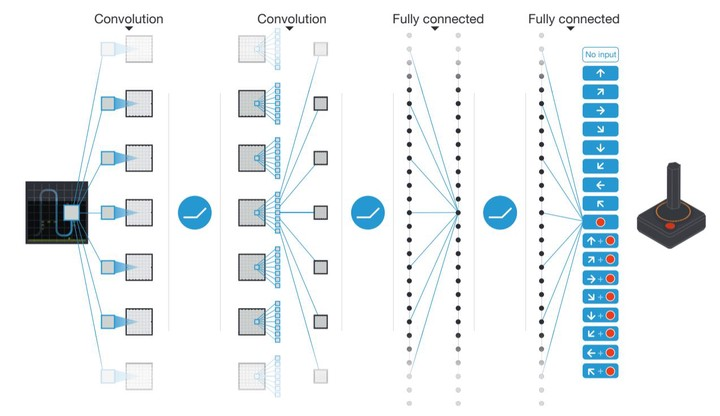
\includegraphics[width=.49\linewidth]{Pic/slide/atari-architect}
		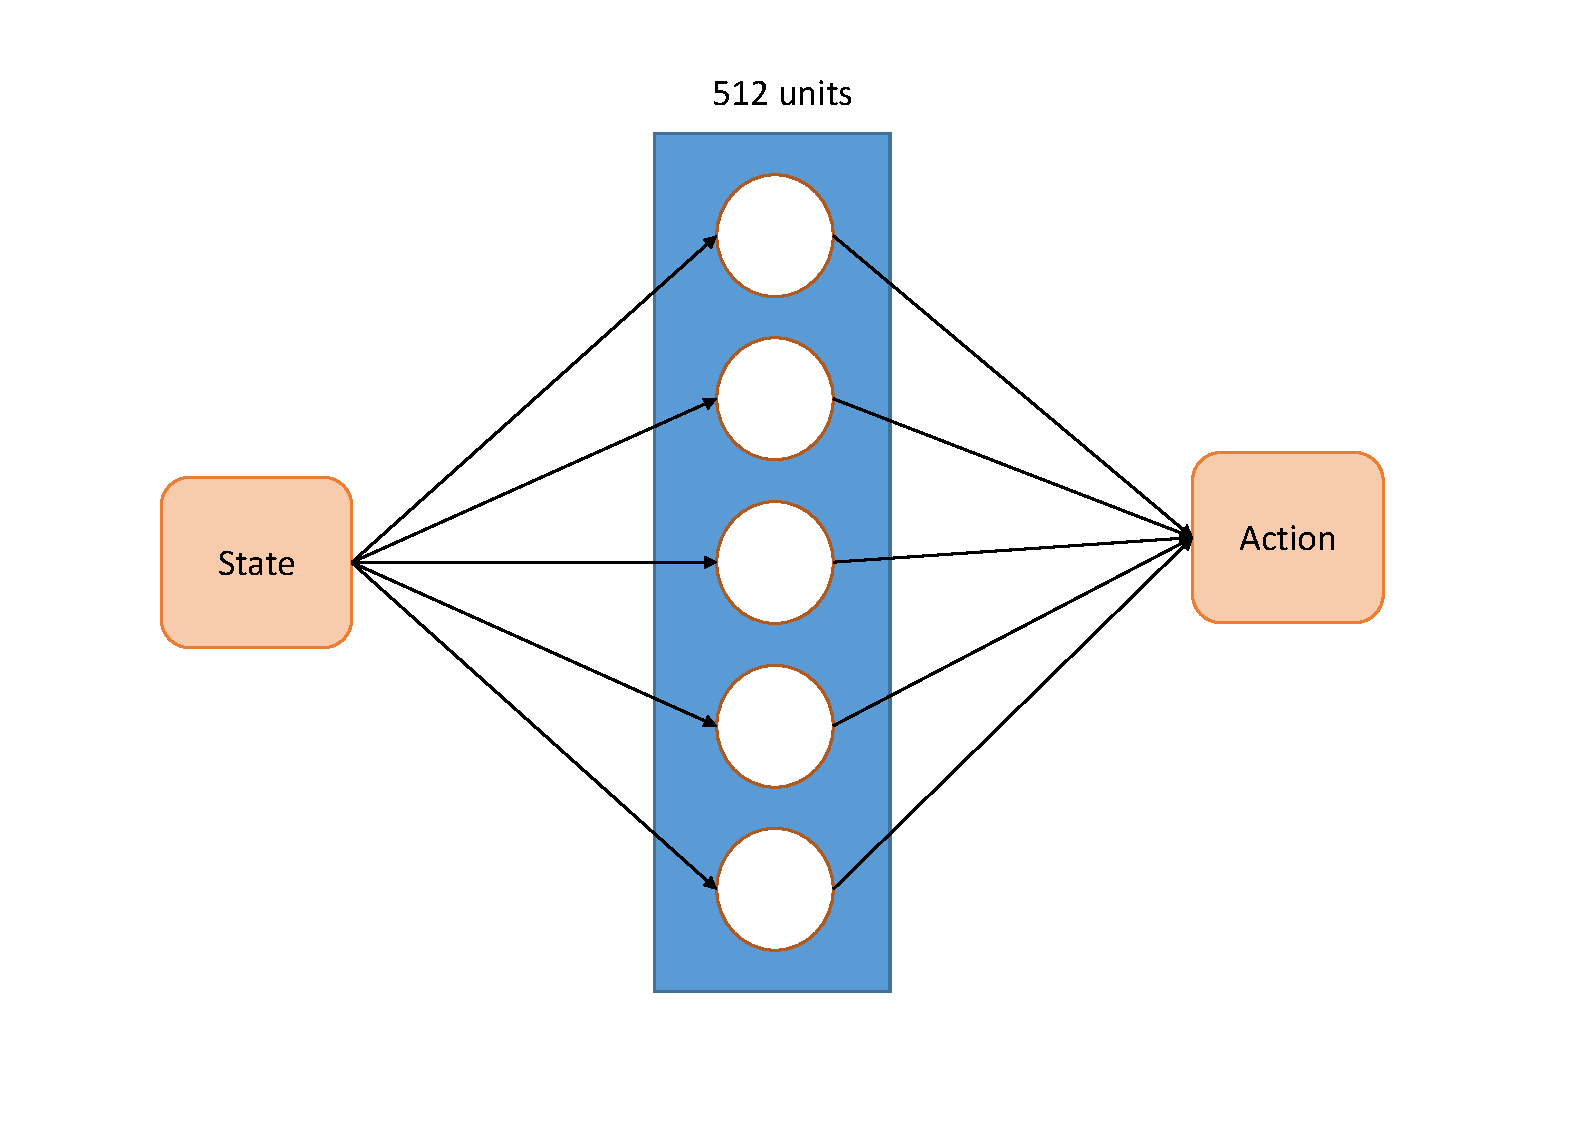
\includegraphics[width=.49\linewidth]{Pic/baseline/baseline_archetect}
	\end{figure}
	Lấy cảm hứng Deepmind, tuy nhiên nhóm tác giả sẽ tự phân tích đặc trưng và đây sẽ là đầu vào của Q-learning.
\end{frame}
%---------------------------------------------------------------%
\begin{frame}{Mô hình đề xuất}
Tỷ lệ thắng 16,0\%.
    \begin{figure}[ht]
    	\centering
    	\begin{subfigure}{.5\textwidth}
    		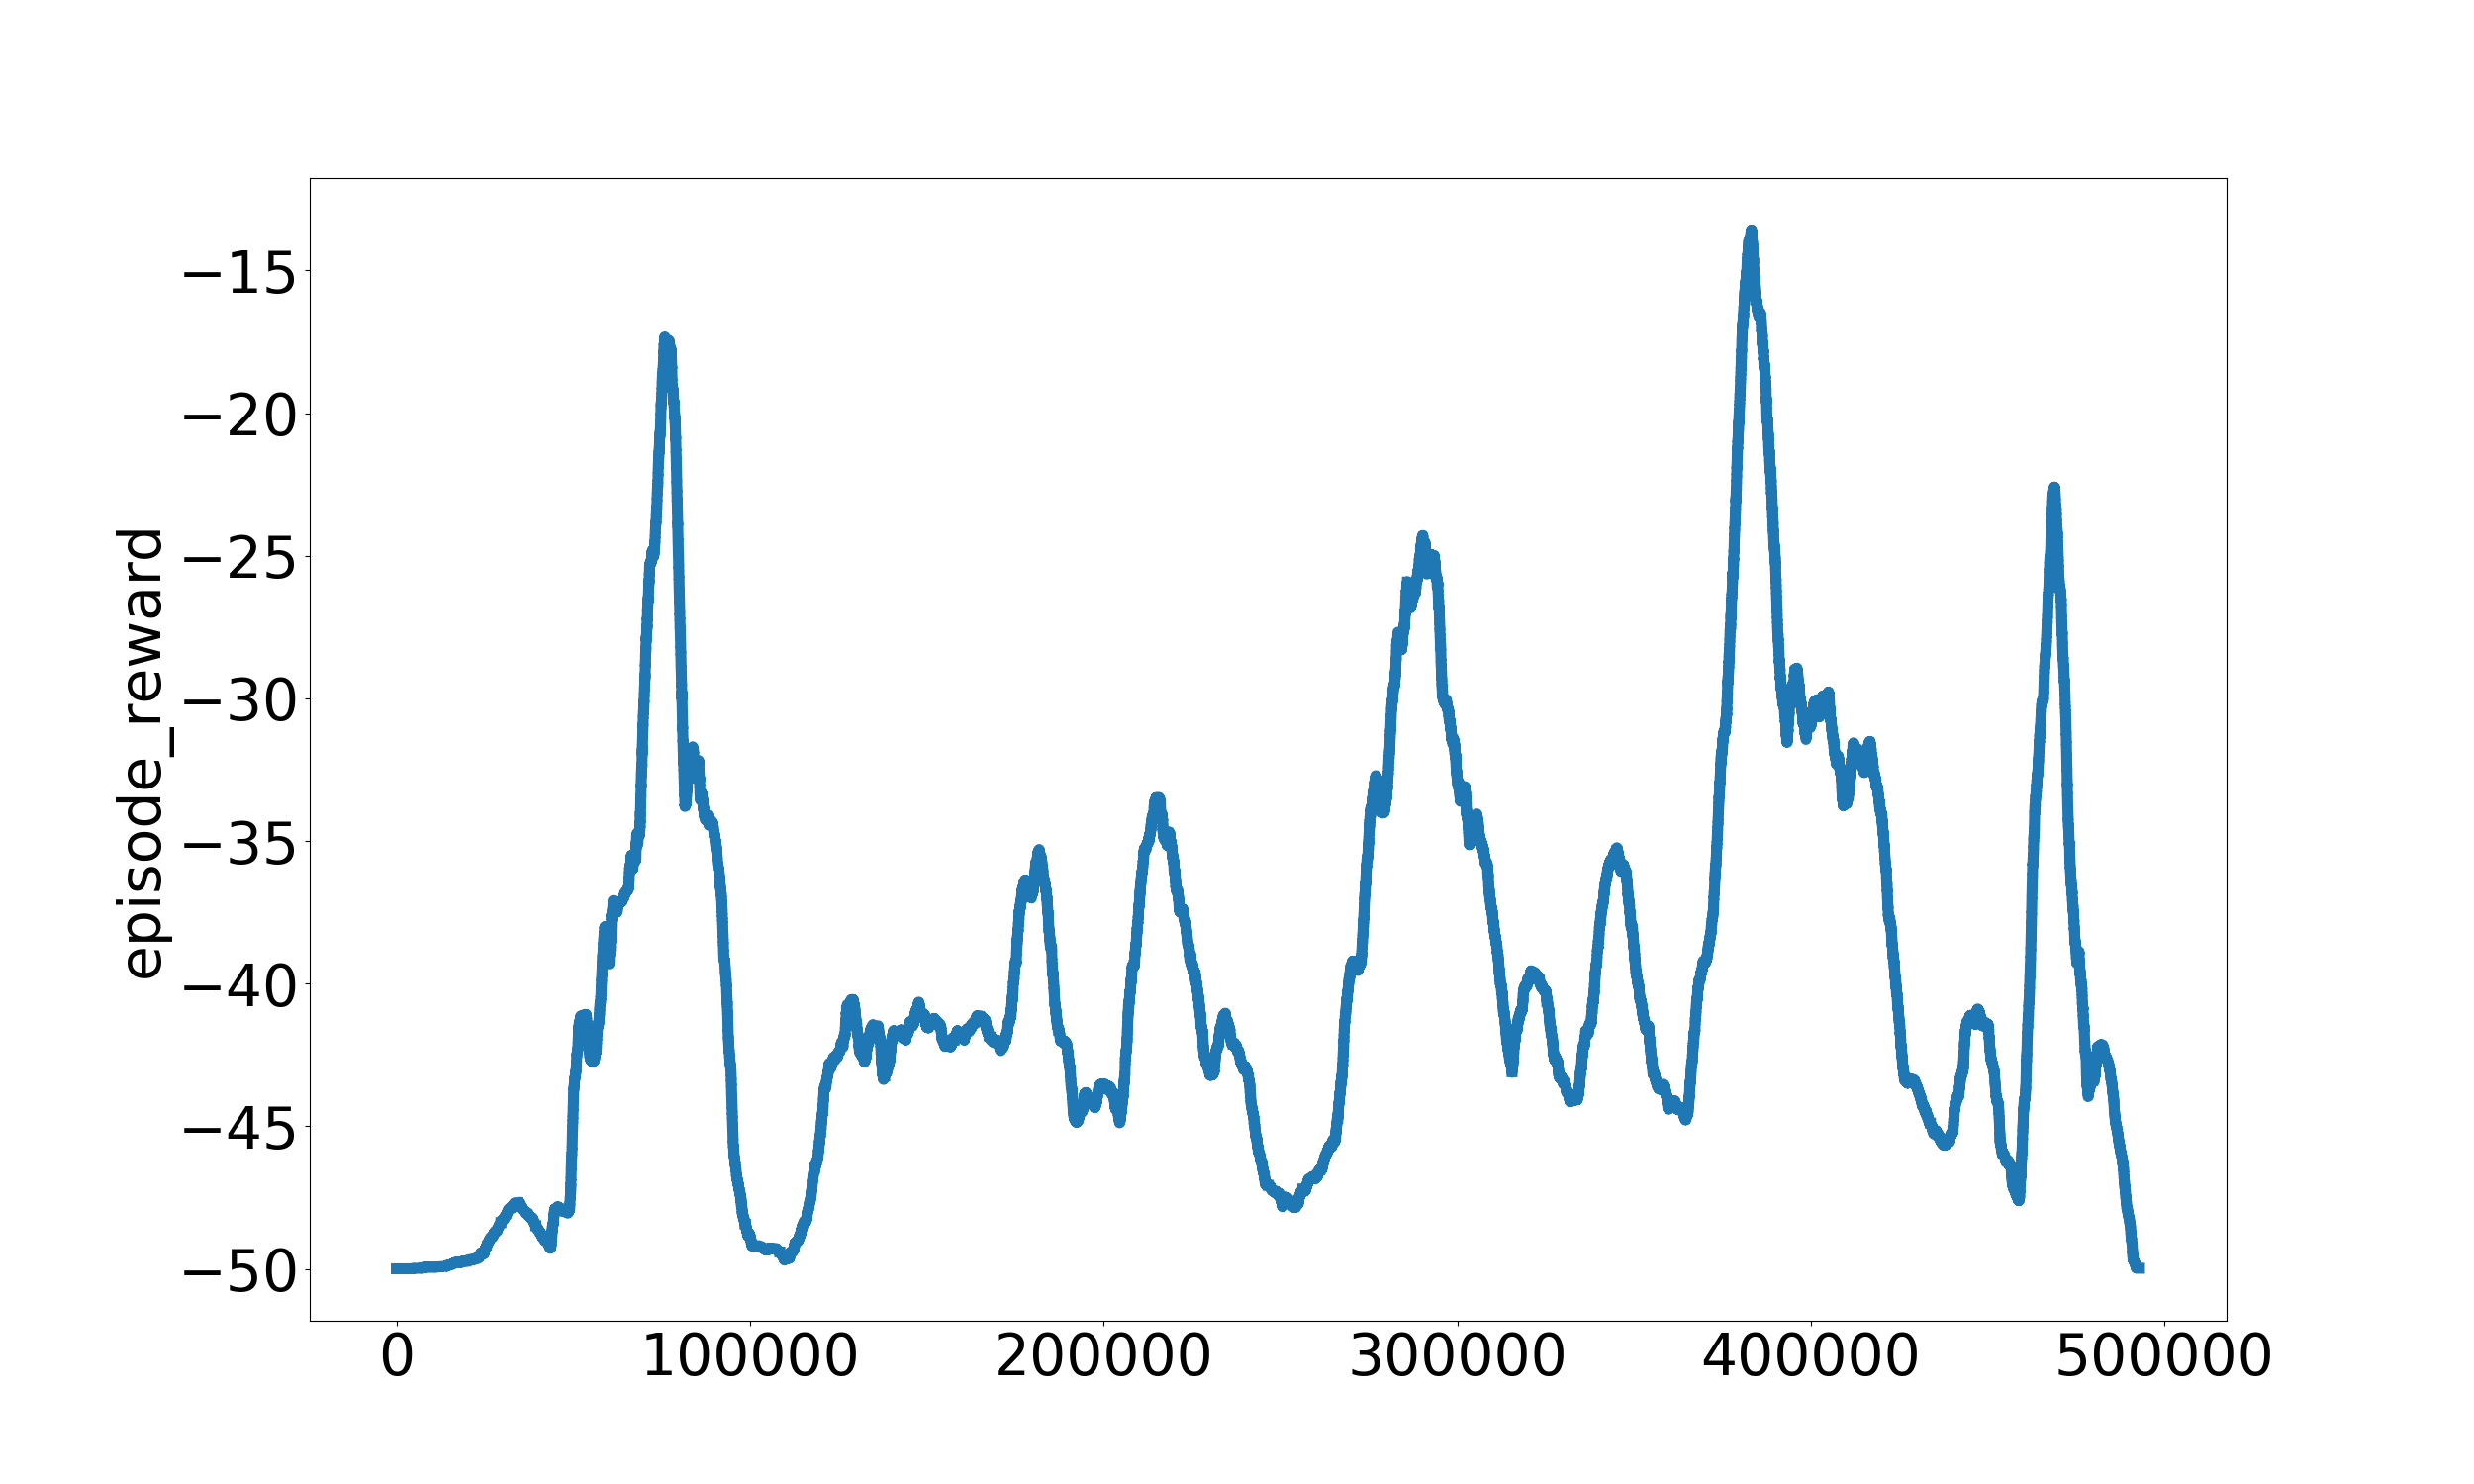
\includegraphics[width=0.9\textwidth]{Pic/baseline/episode_reward.png}  
    		\caption{Trung bình tích lũy phần thưởng}
    		\label{fig:baseline_avg}
    	\end{subfigure}%
    	\begin{subfigure}{.5\textwidth}
    		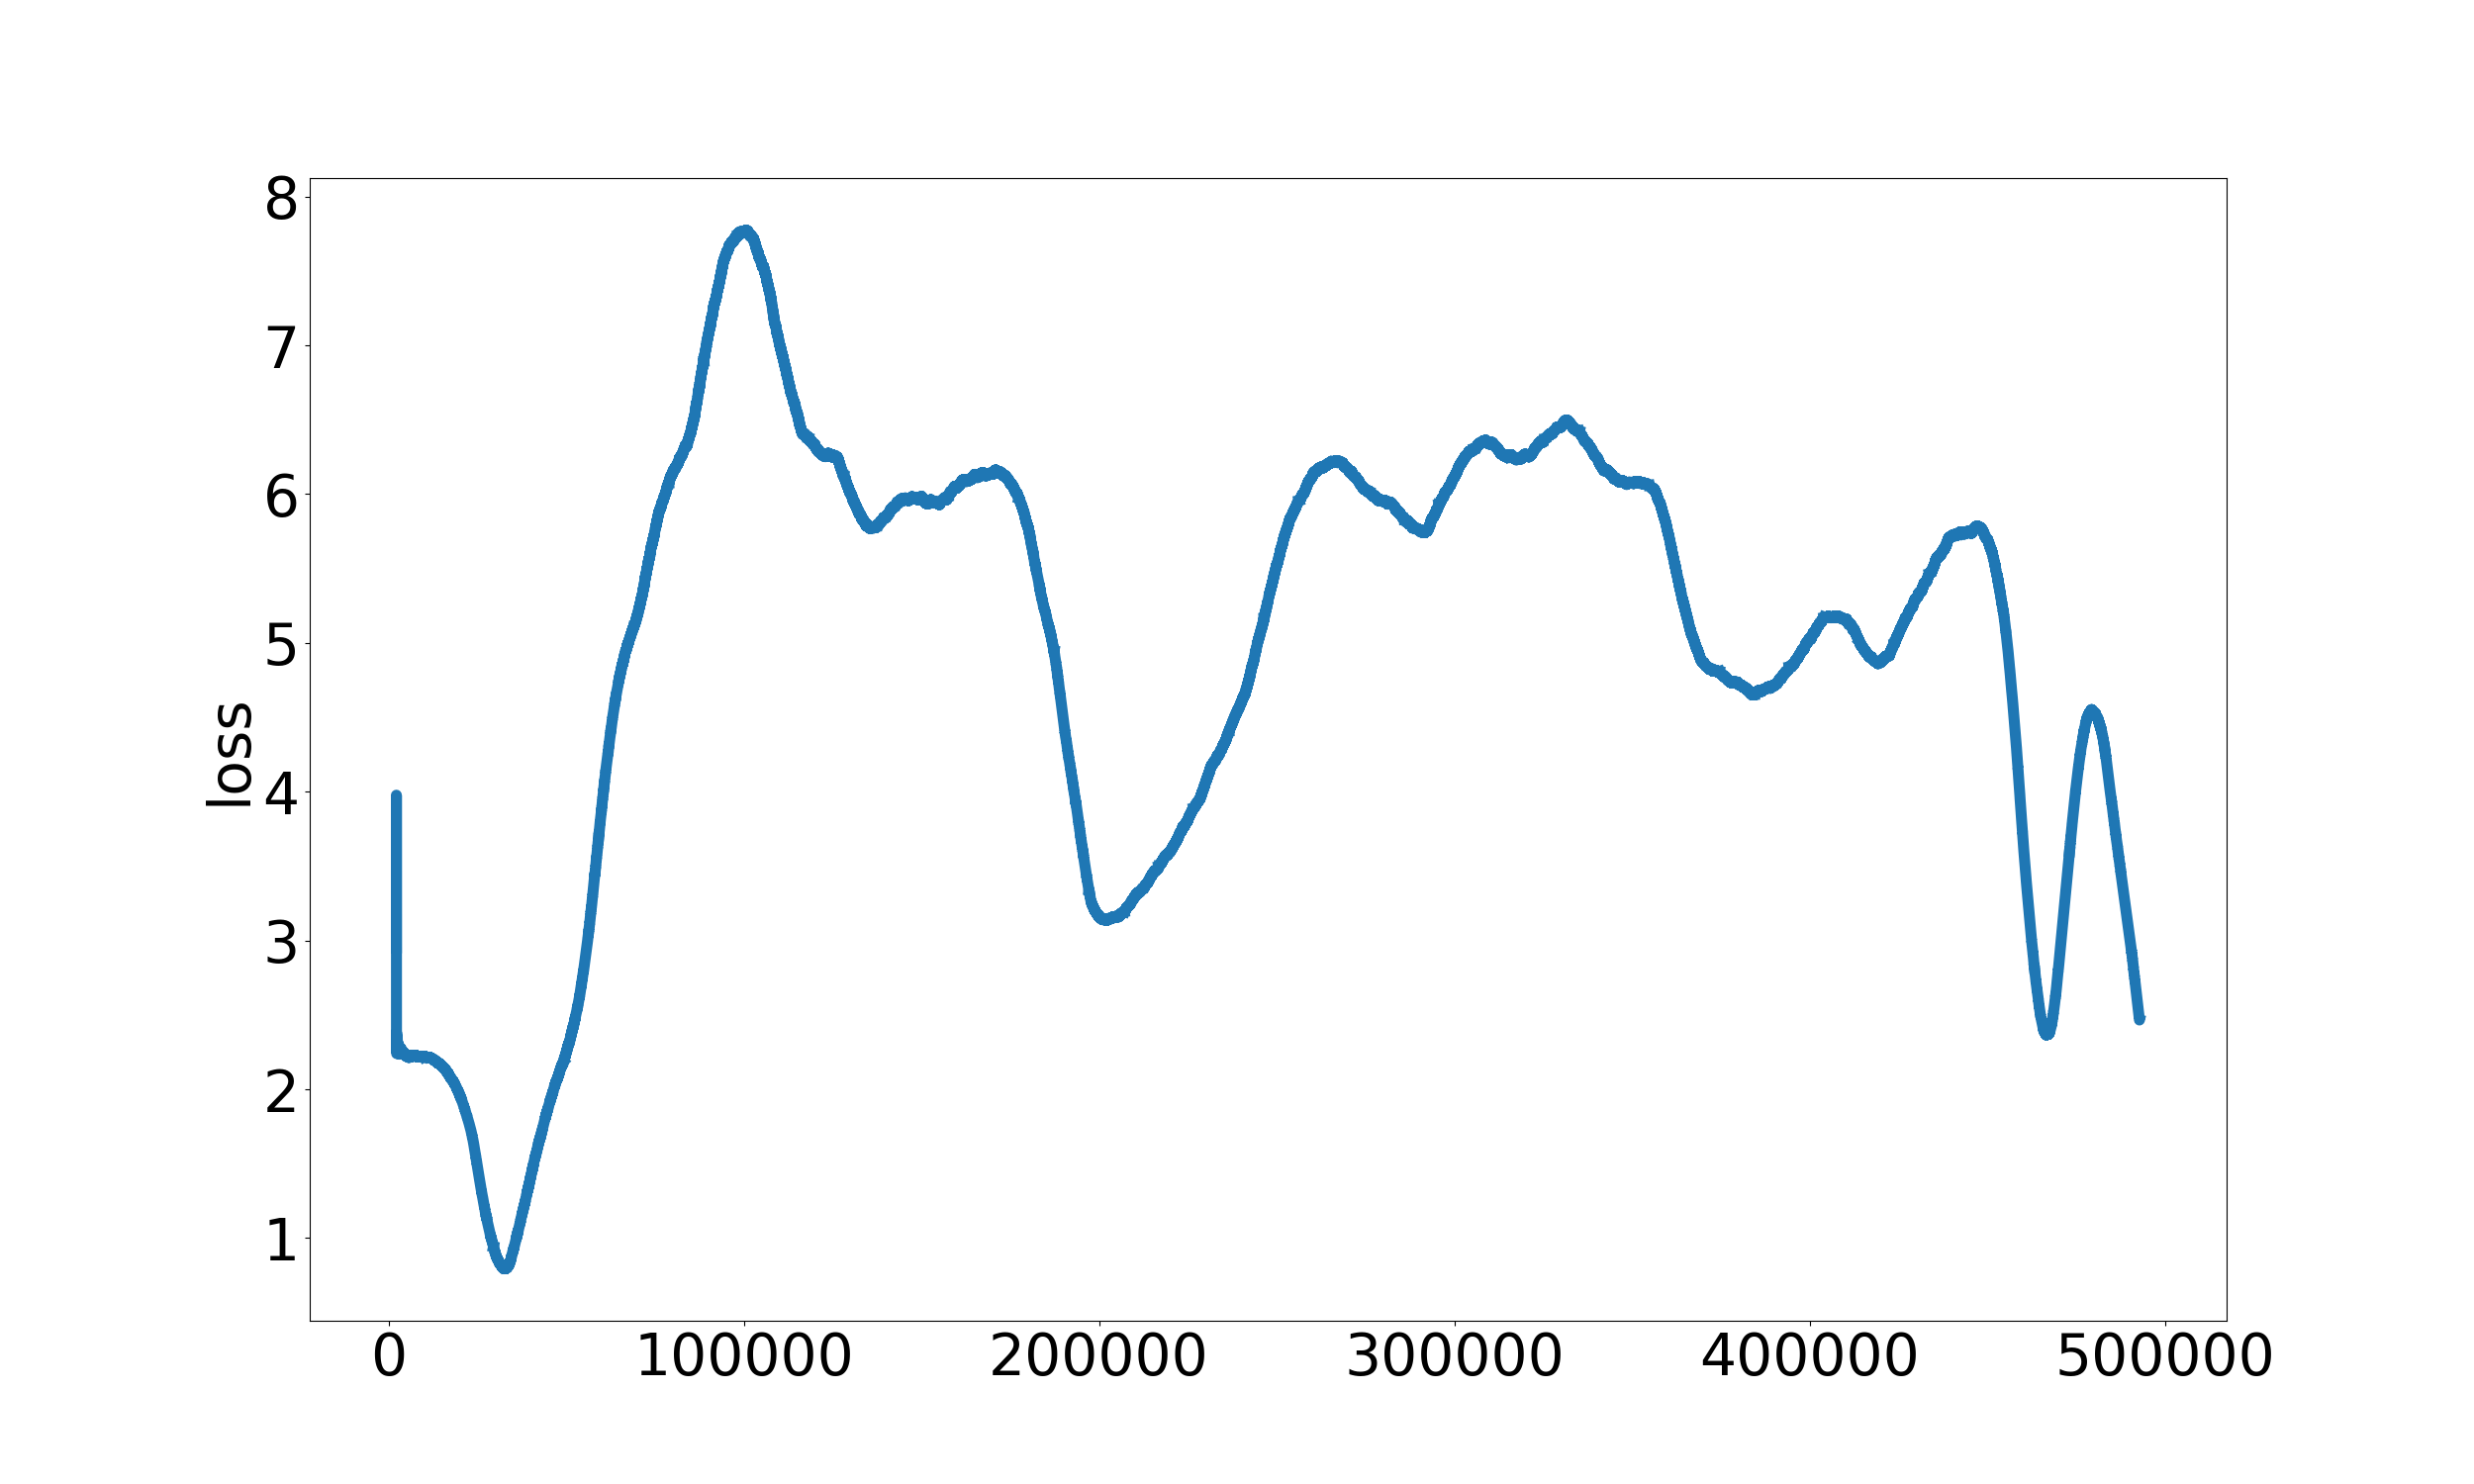
\includegraphics[width=.9\textwidth]{Pic/baseline/loss.png}  
    		\caption{Hàm mất mát}
    		\label{fig:baseline_loss}
    	\end{subfigure}\\
    	\begin{subfigure}{.5\textwidth}
    		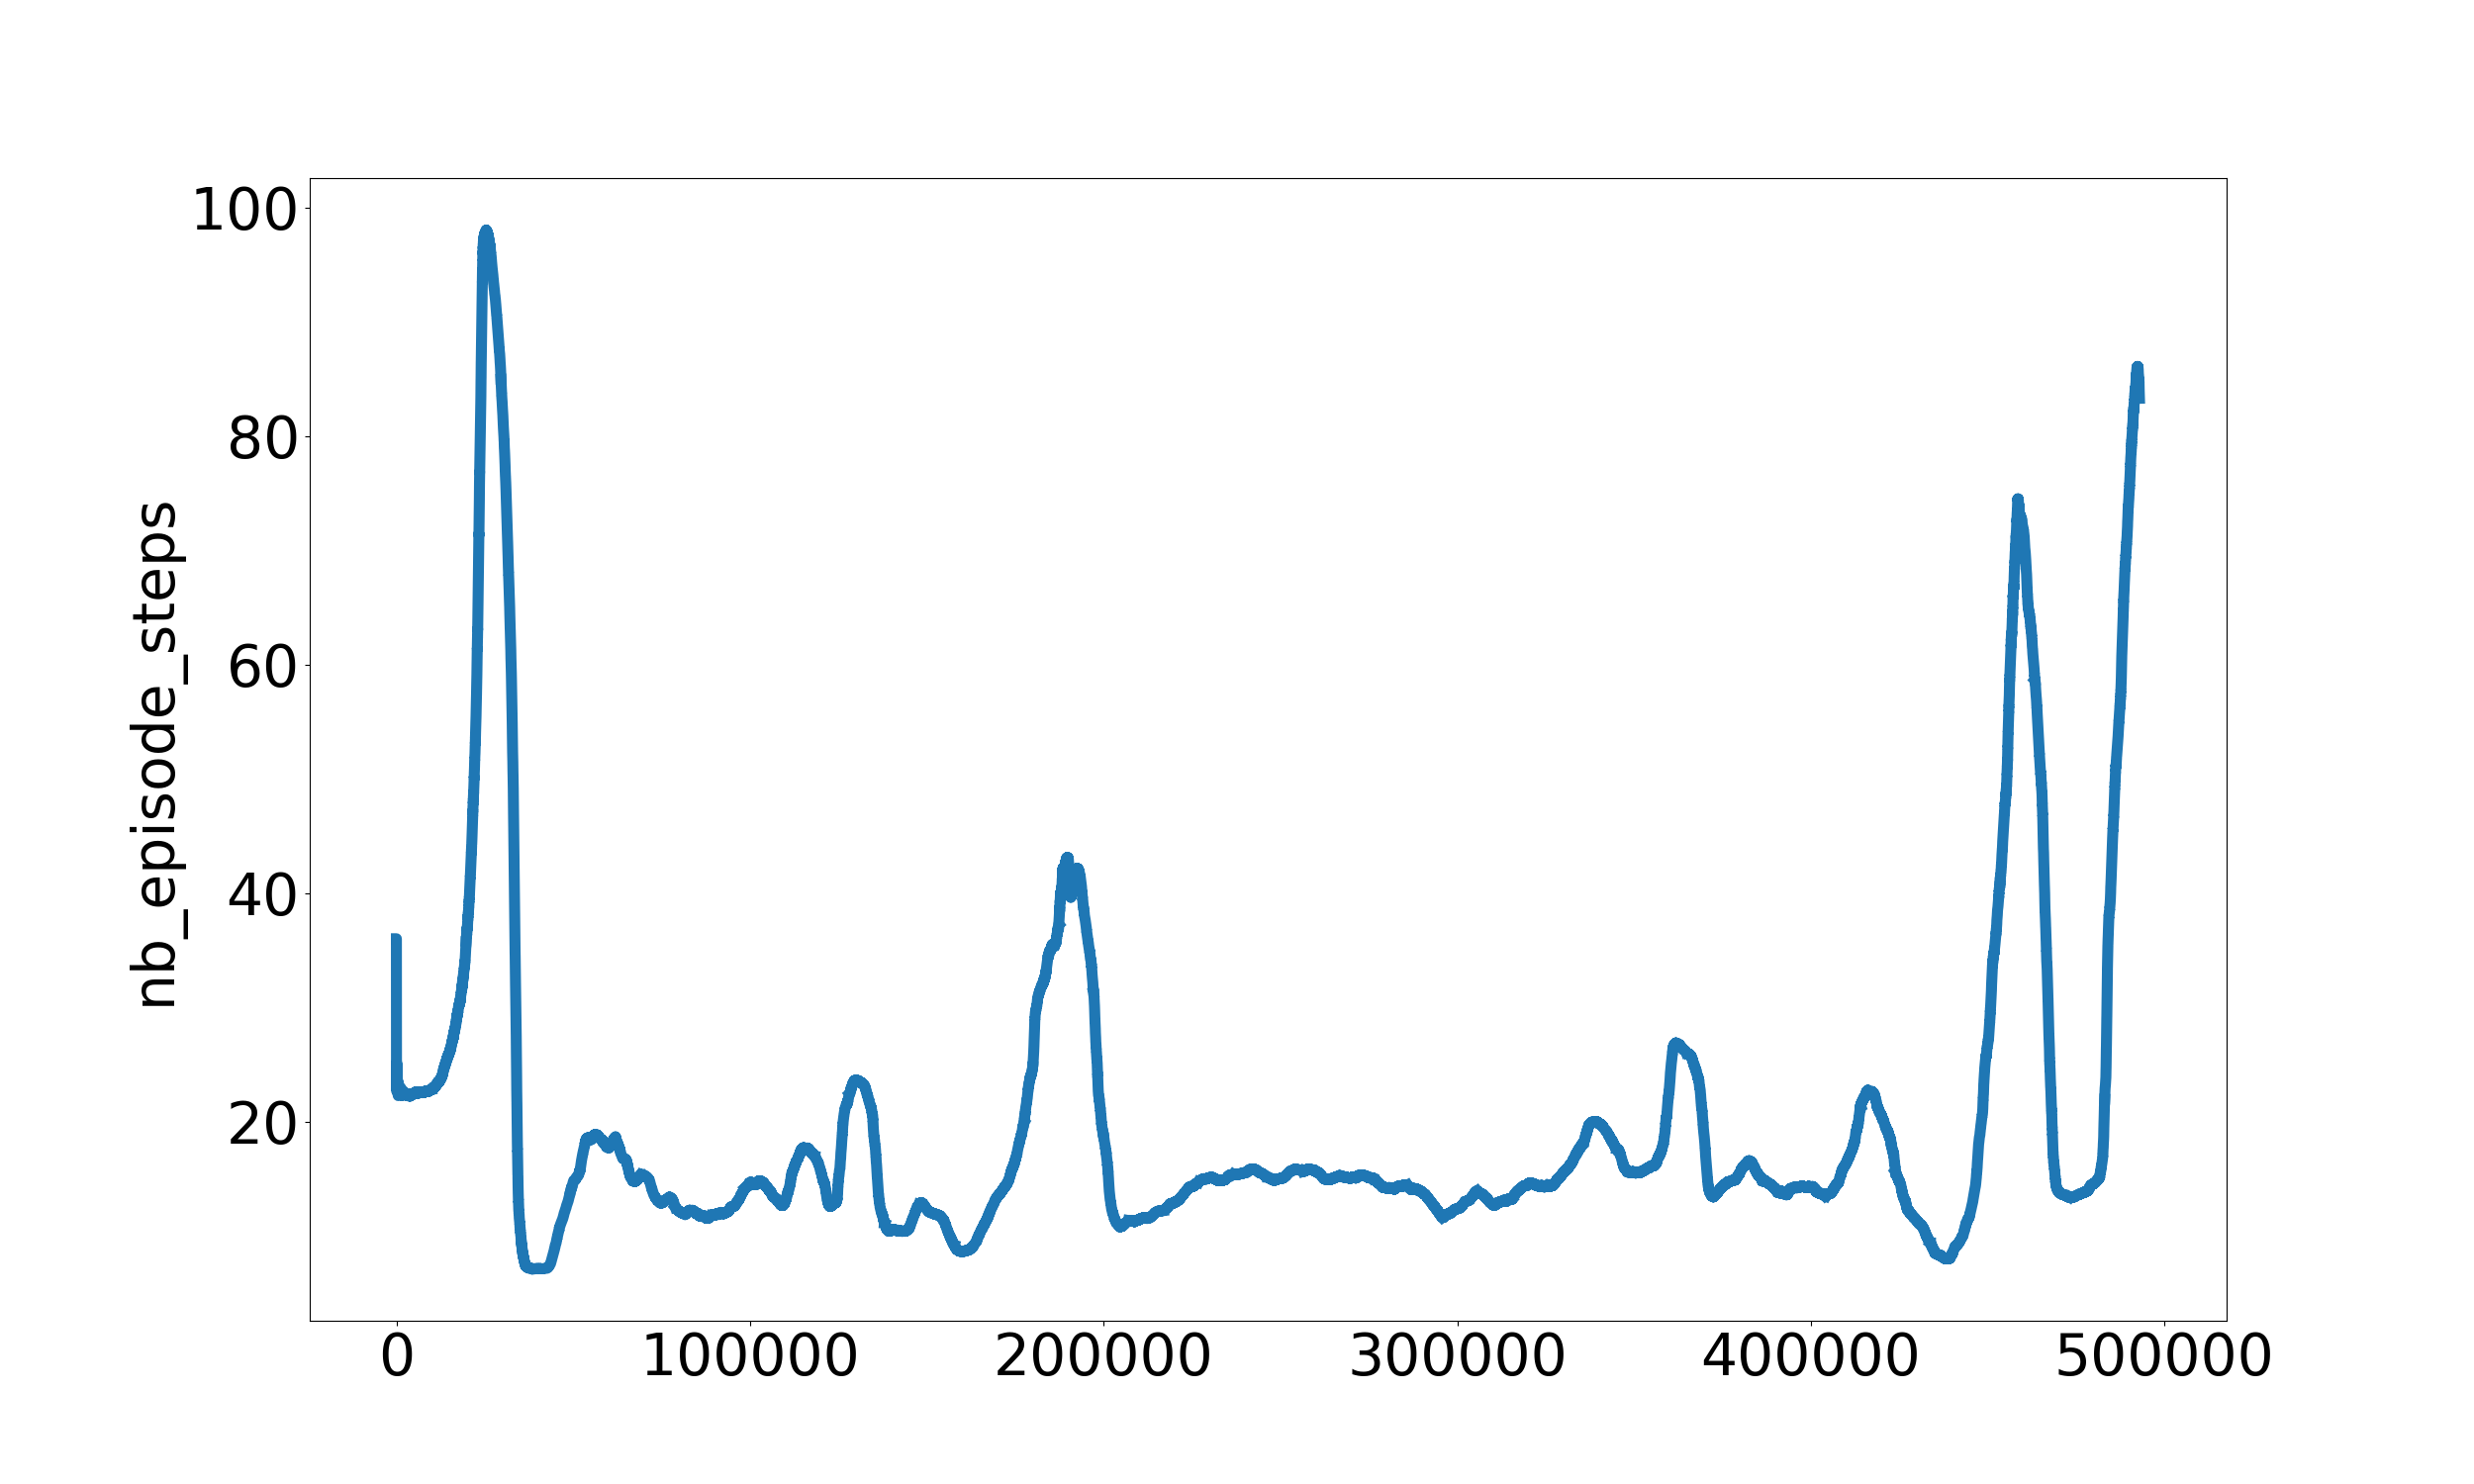
\includegraphics[width=.9\textwidth]{Pic/baseline/nb_episode_steps.png}
    		\caption{Số bước thực hiện}
    		\label{fig:baseline_step}
    	\end{subfigure}%
    	\begin{subfigure}{.5\textwidth}
    		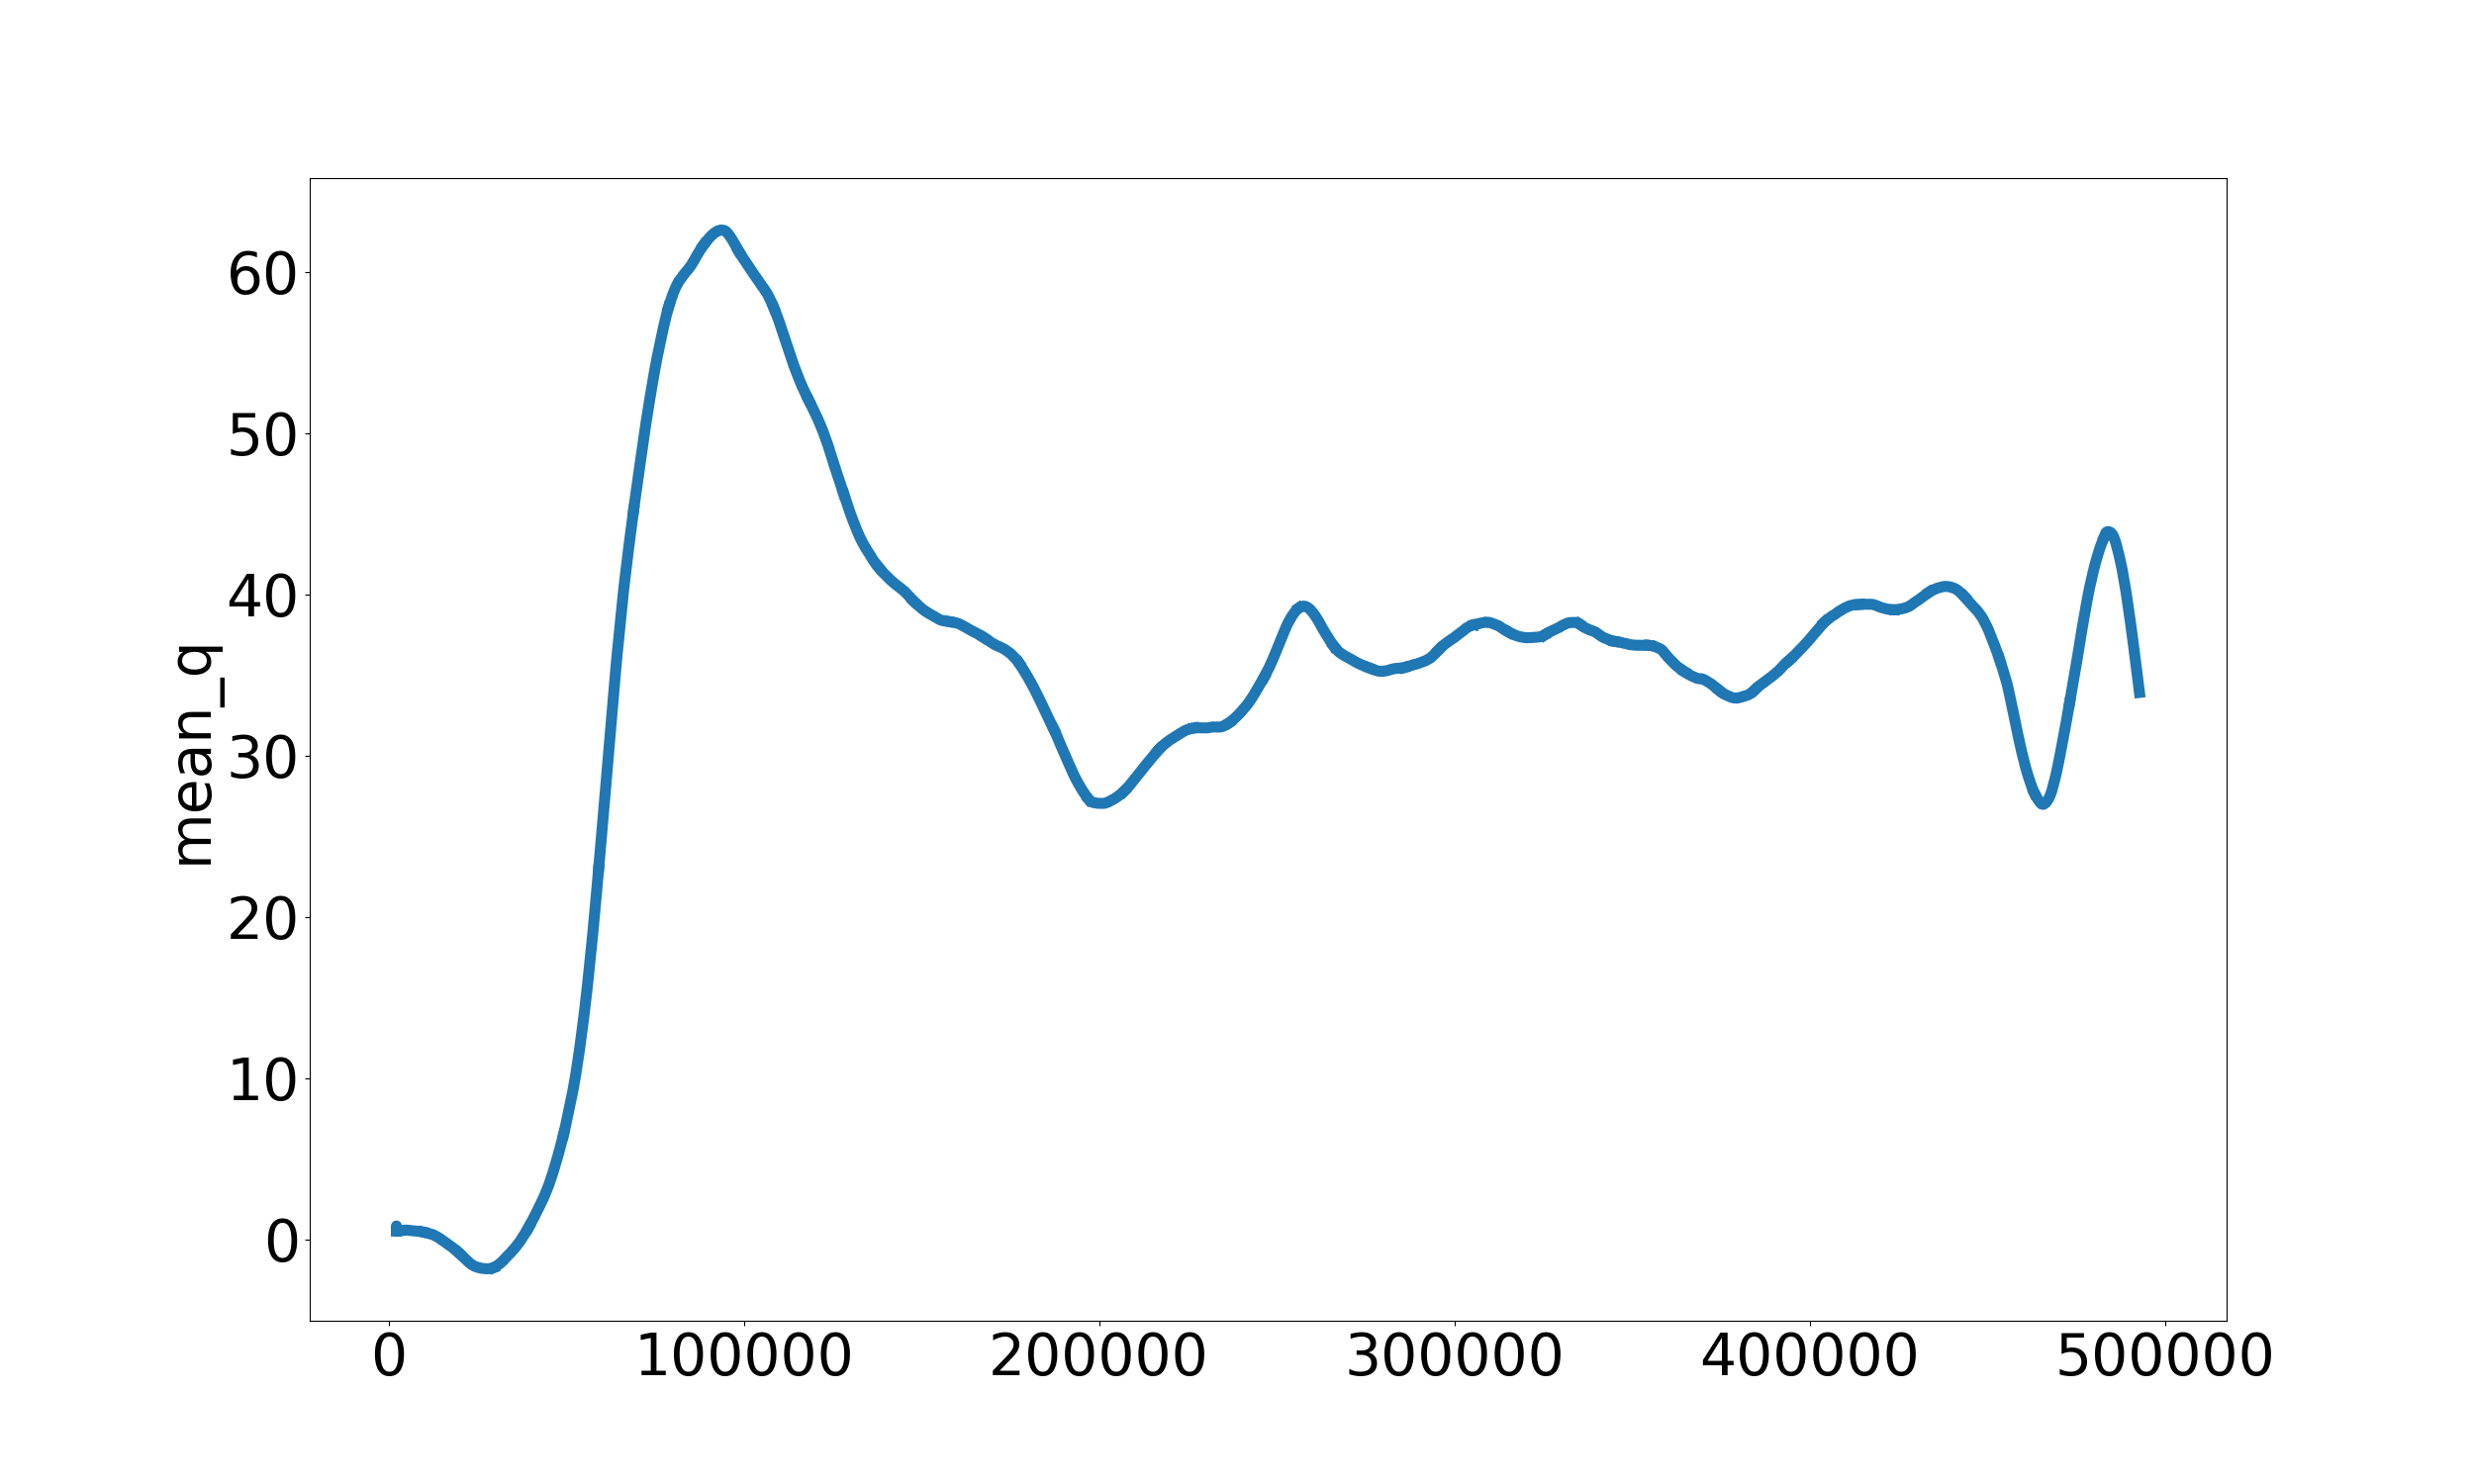
\includegraphics[width=.9\textwidth]{Pic/baseline/mean_q.png}  
    		\caption{Trung bình giá trị Q}
    		\label{fig:baseline_mean_q}
    	\end{subfigure}
    	\label{fig:result_baseline}
    \end{figure}
\end{frame}
%---------------------------------------------------------------%
\subsection{Một số thử nghiệm}
\begin{frame}{Phương pháp và kết quả}
	\centering
	\huge\textbf{MỘT SỐ THỬ NGHIỆM}
	\vfill
	\begin{itemize}
	    \item \small I.  Mô hình thứ nhất 
	    \item \small II. Mô hình thứ hai
	\end{itemize}
\end{frame}
%---------------------------------------------------------------%
\begin{frame}{Một số thử nghiệm}
    \textbf{Mô hình thứ nhất}
    \vspace{0.5cm}
    \begin{itemize}
        \item 1. Thay đổi hàm phần thưởng
        \vspace{0.5cm}
        \item 2. Thay đổi cách khám phá môi trường
        \vspace{.5cm}
        \item 3. Thay đổi cấu trúc mô hình
    \end{itemize}
\end{frame}
%---------------------------------------------------------------%
\begin{frame}{Mô hình thứ nhất}
1. Thay đổi hàm phần thưởng:\\
\begin{subnumcases}{r(s_t,a_t,s_{t+1})=}
        +R_{0} & $s_{t+1}=\text{đích}$ \nonumber\\
        -R_{1} & $s_{t+1}=\text{chết}$\nonumber\\
        -d(s_{t+1}) & còn lại\nonumber
    \end{subnumcases}
\end{frame}
%---------------------------------------------------------------%
\begin{frame}{Mô hình thứ nhất}
2. Thay đổi cách khám phá môi trường:
	\begin{figure}
		\centering
		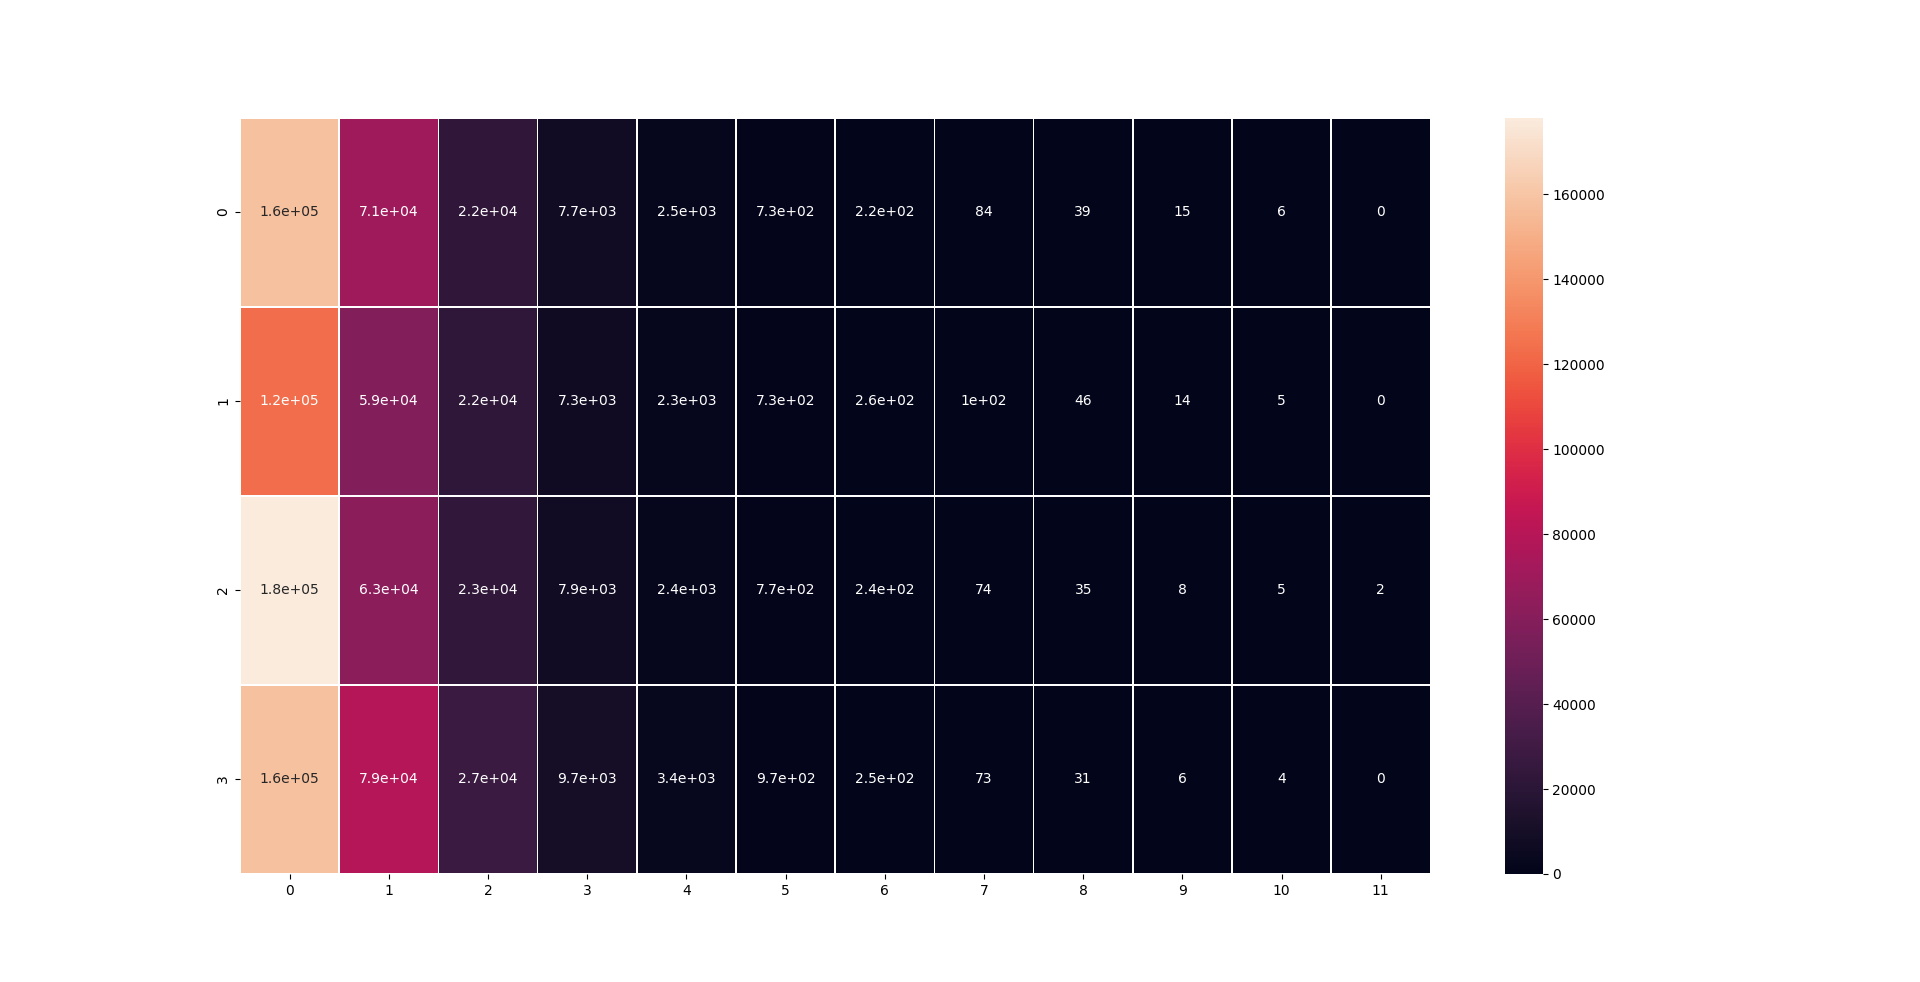
\includegraphics[width=\linewidth]{Pic/First_model/agent_pos_before.png}
	\end{figure}
\end{frame}
%---------------------------------------------------------------%
\begin{frame}{Mô hình thứ nhất}
2. Thay đổi cách khám phá môi trường:
	\begin{figure}
		\centering
		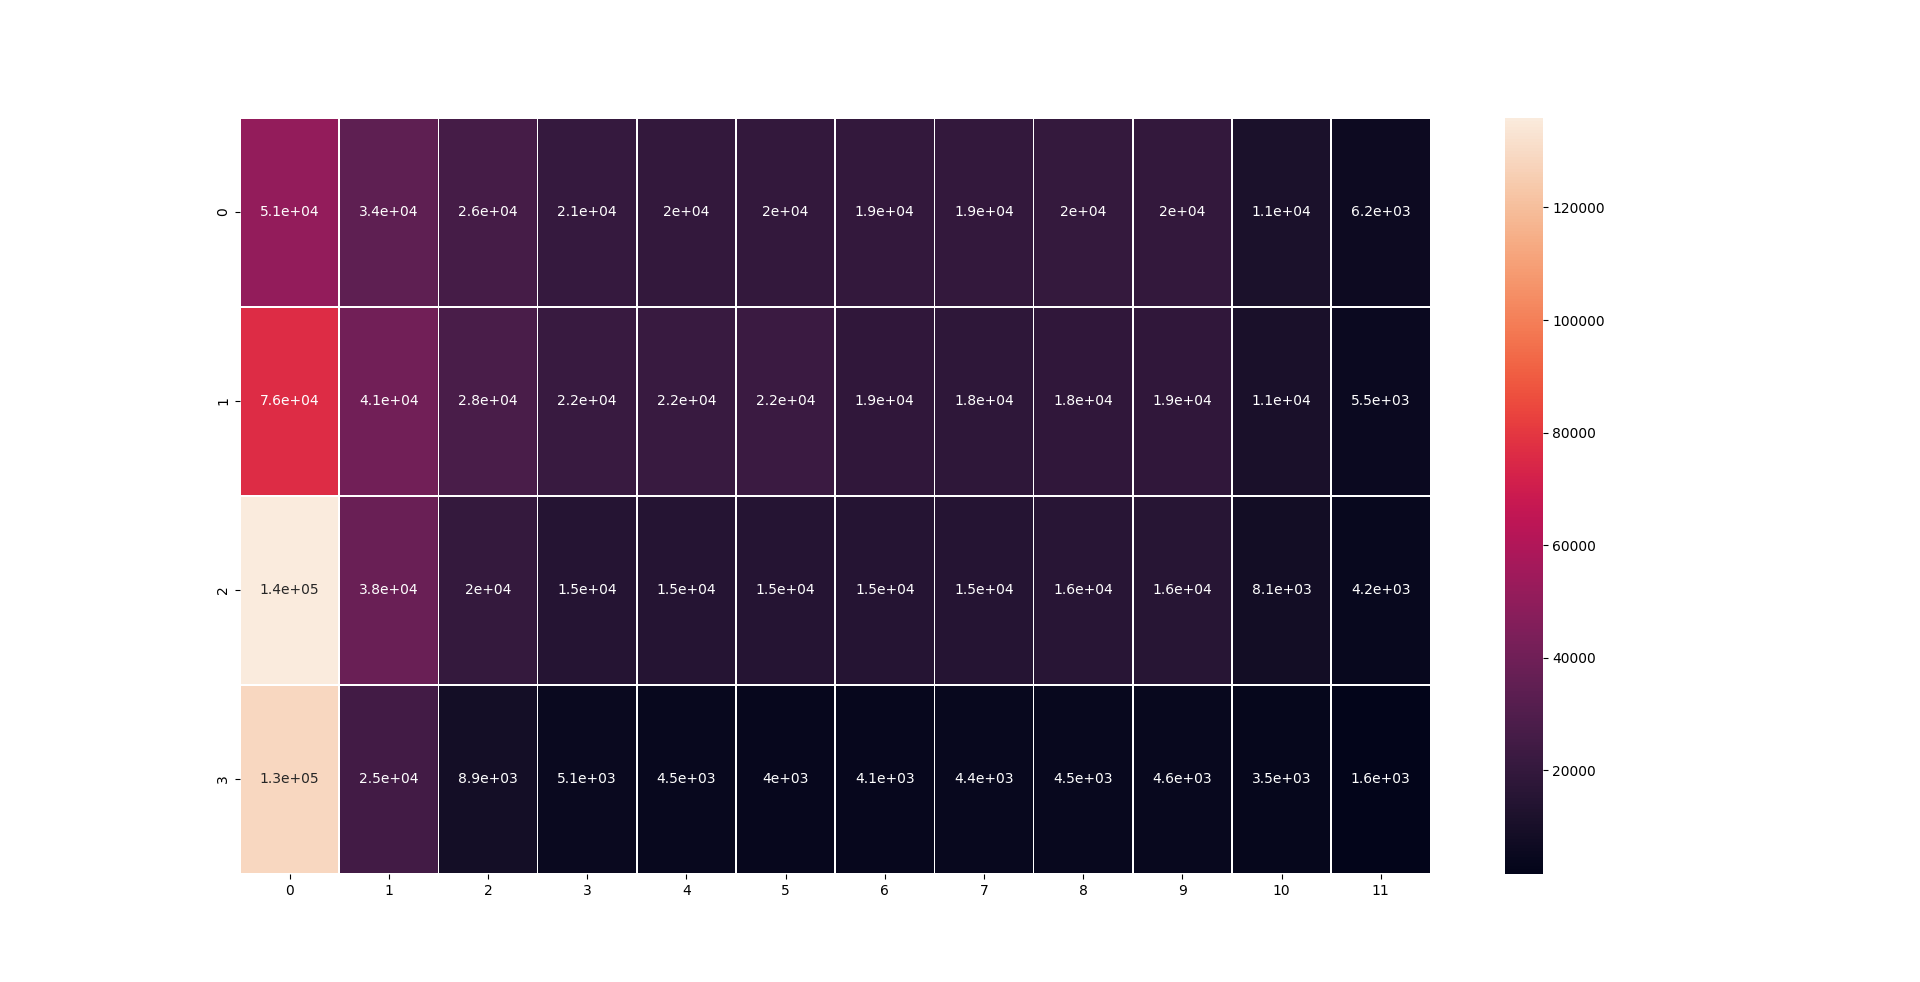
\includegraphics[width=\linewidth]{Pic/First_model/agent_pos_after.png}
	\end{figure}
\end{frame}
%---------------------------------------------------------------%
\begin{frame}{Mô hình thứ nhất}
3. Thay đổi cấu trúc mô hình\\
	Thay vì sử dụng một lớp ẩn 512 phần tử, nhóm tác giảm xuống 64 phần tử vì trạng thái đầu vào có kích thước 14.
\end{frame}
%---------------------------------------------------------------%
\begin{frame}{Mô hình thứ nhất}
Lần 1\\
    \begin{subnumcases}{r(s_t,a_t,s_{t+1})=}
        +10 & $s_{t+1}=\text{đích}$\nonumber \\
        -10 & $s_{t+1}=\text{chết}$\nonumber\\
        -d(s_{t+1}) & còn lại\nonumber
    \end{subnumcases}
    Với
    \[d(s_{t+1}) = \frac{\text{vị trí cột đích}-\text{vị trí cột trạng thái tiếp theo}}{\text{\text{vị trí cột đích} - \text{vị trí cột bắt đầu}}}\]
\end{frame}
%---------------------------------------------------------------%
\begin{frame}{Mô hình thứ nhất}
Lần 1, Tỷ lệ thắng 50,6\%.
\begin{figure}[ht]
    	\centering
    	\begin{subfigure}{.5\textwidth}
    		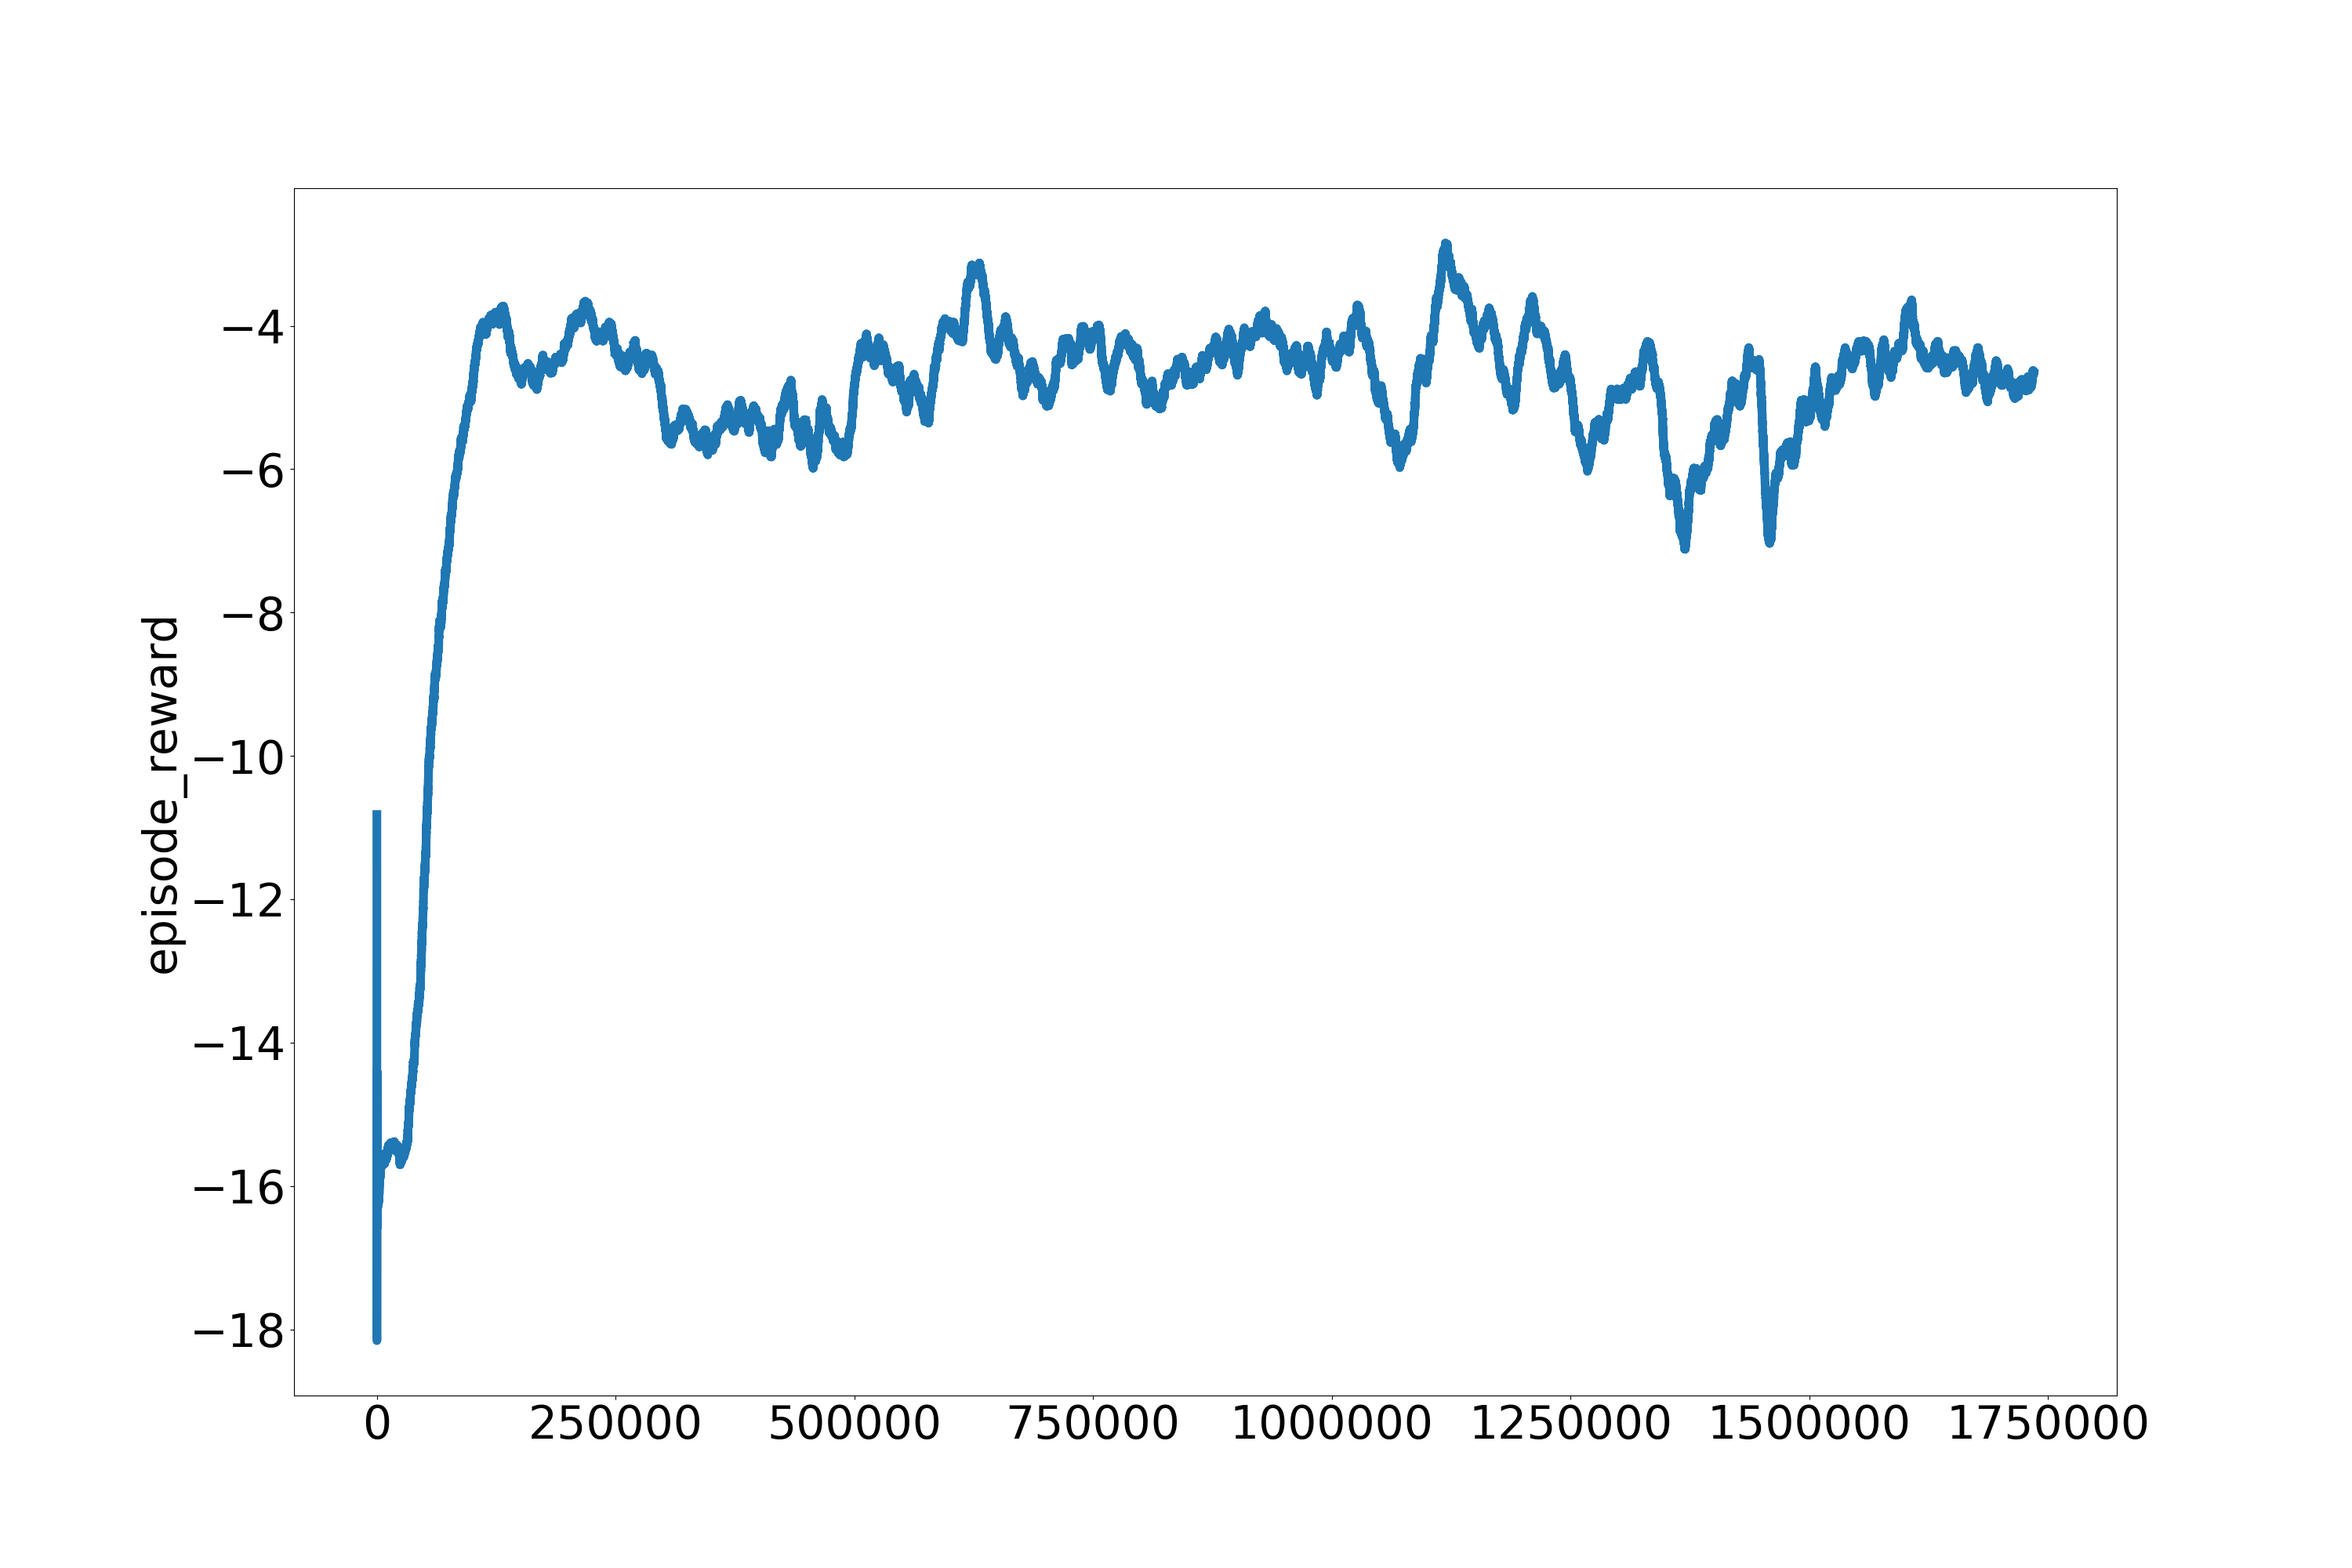
\includegraphics[width=0.85\textwidth]{Pic/First_model/episode_reward.png}
    		\caption{Trung bình tích lũy phần thưởng}
    		\label{fig:baseline_avg}
    	\end{subfigure}%
    	\begin{subfigure}{.5\textwidth}
    		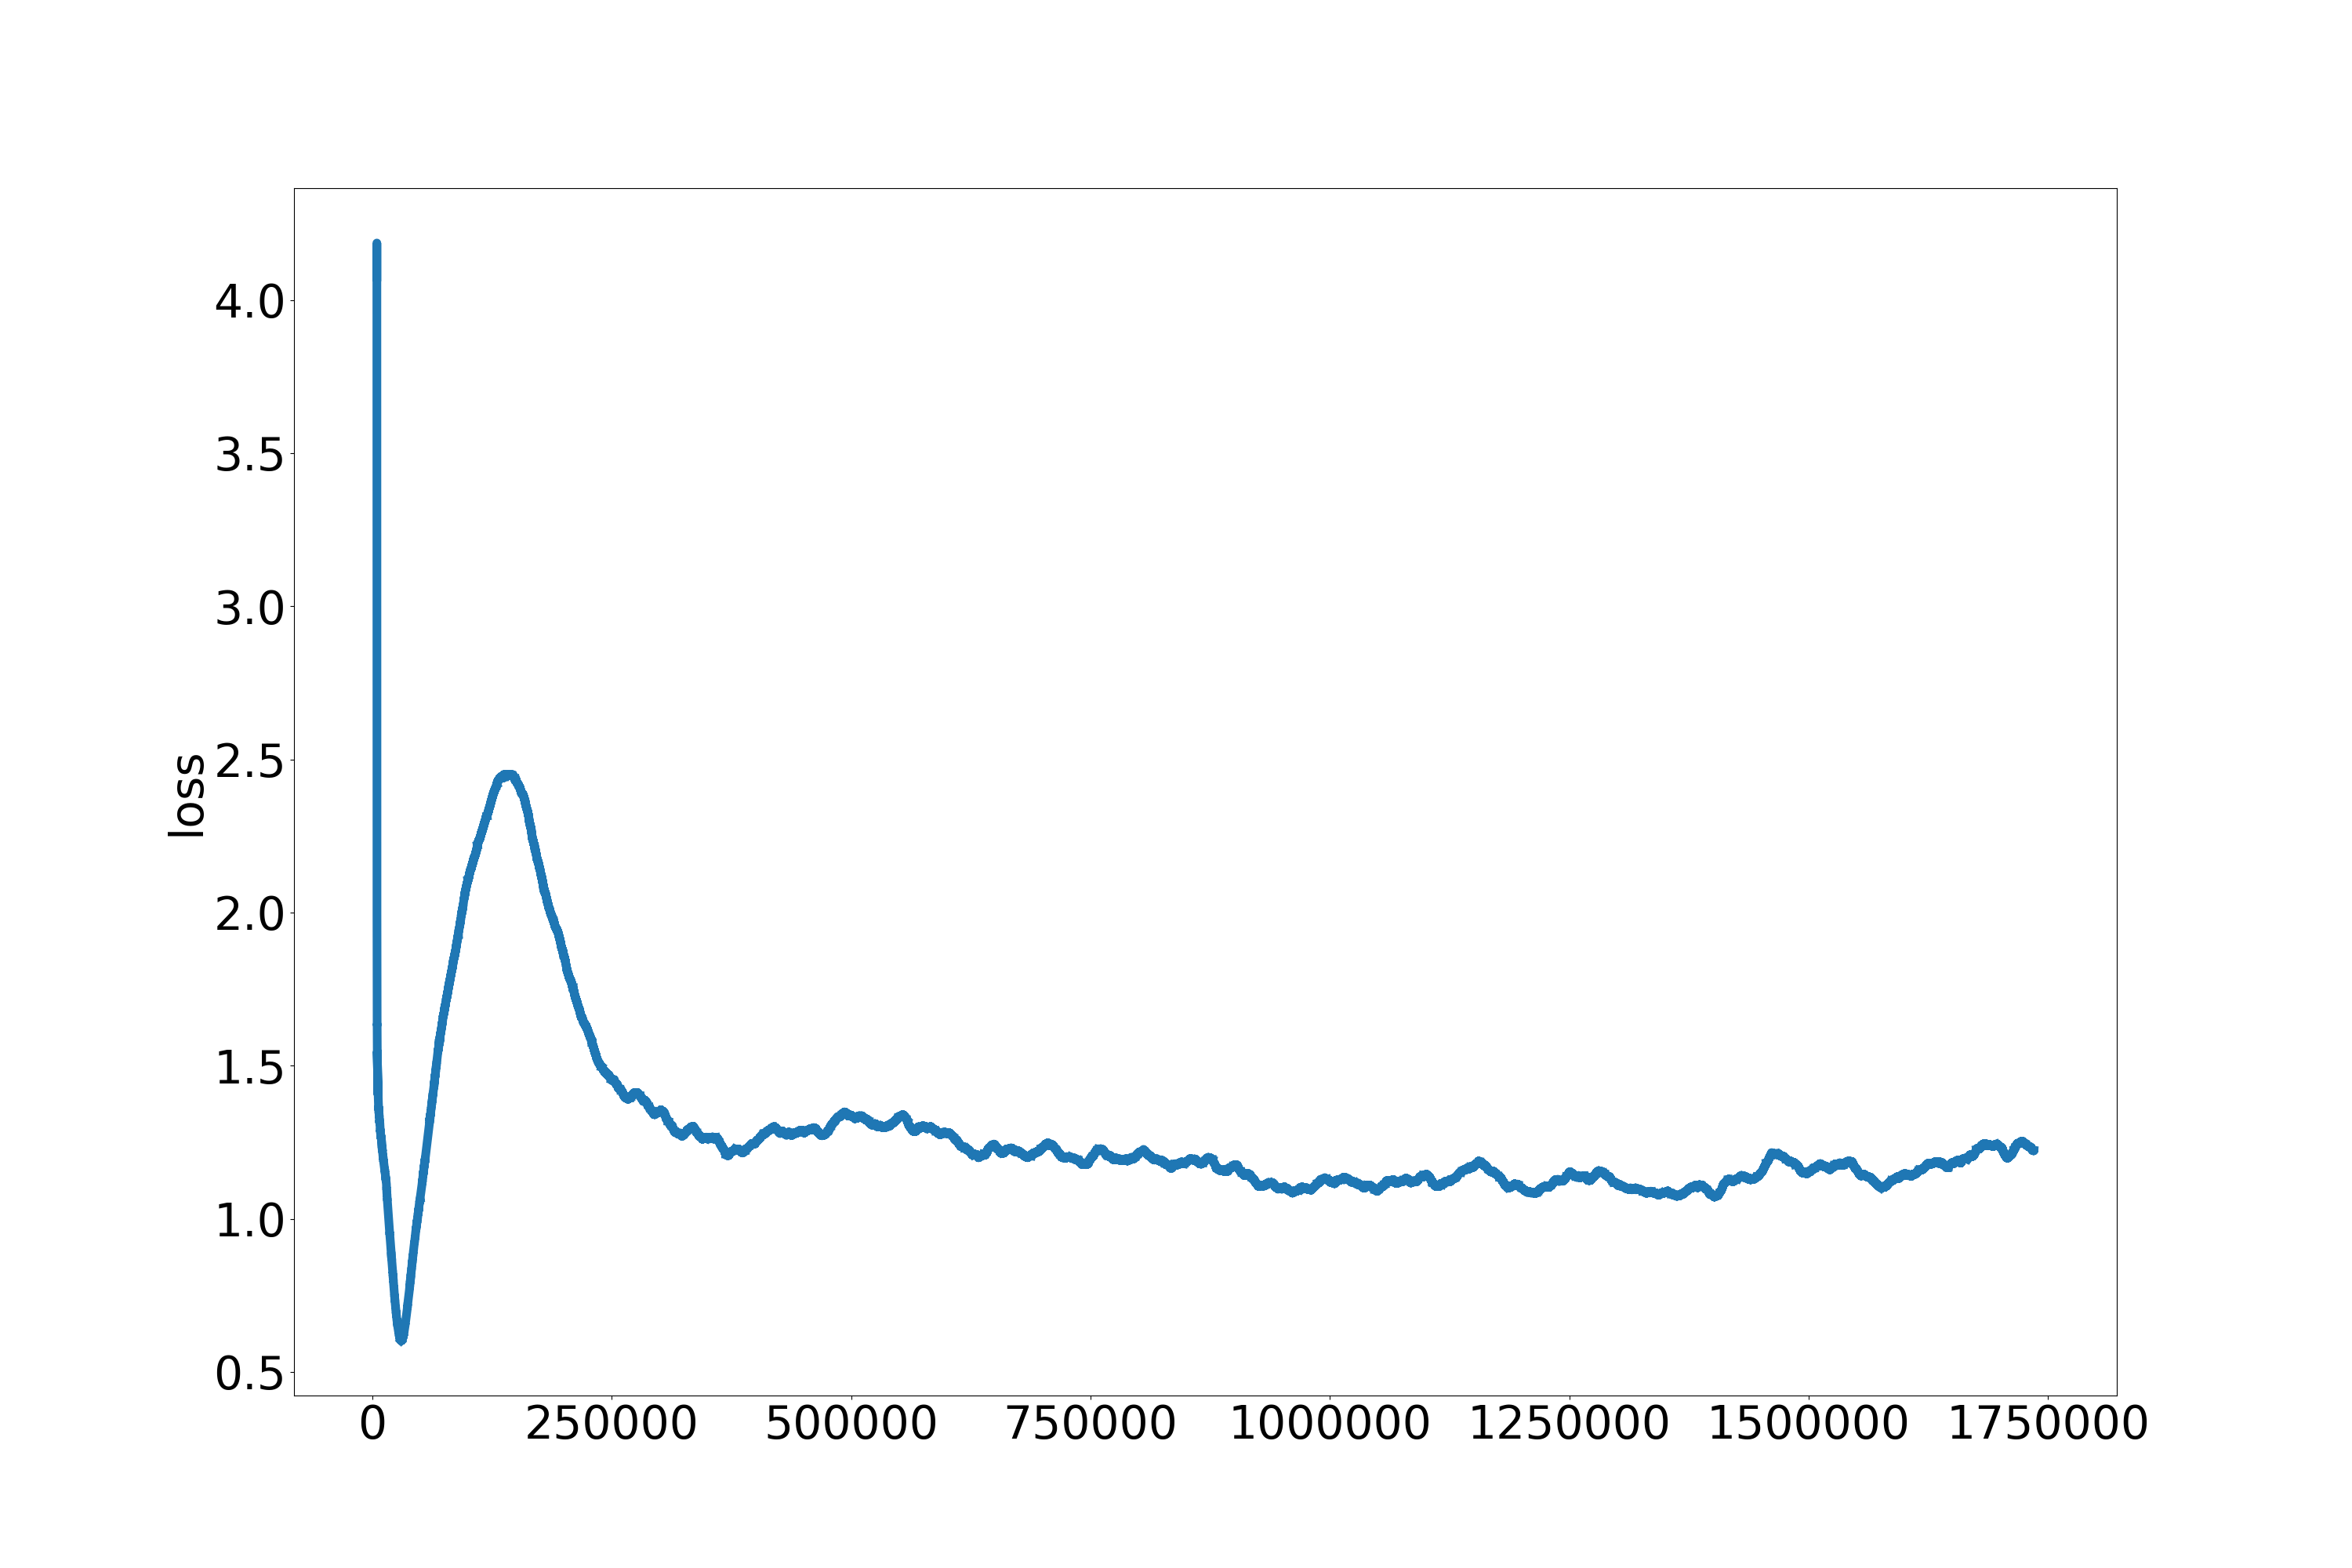
\includegraphics[width=0.85\textwidth]{Pic/First_model/loss.png}
    		\caption{Hàm mất mát}
    		\label{fig:baseline_loss}
    	\end{subfigure}\\
    	\begin{subfigure}{.5\textwidth}
    		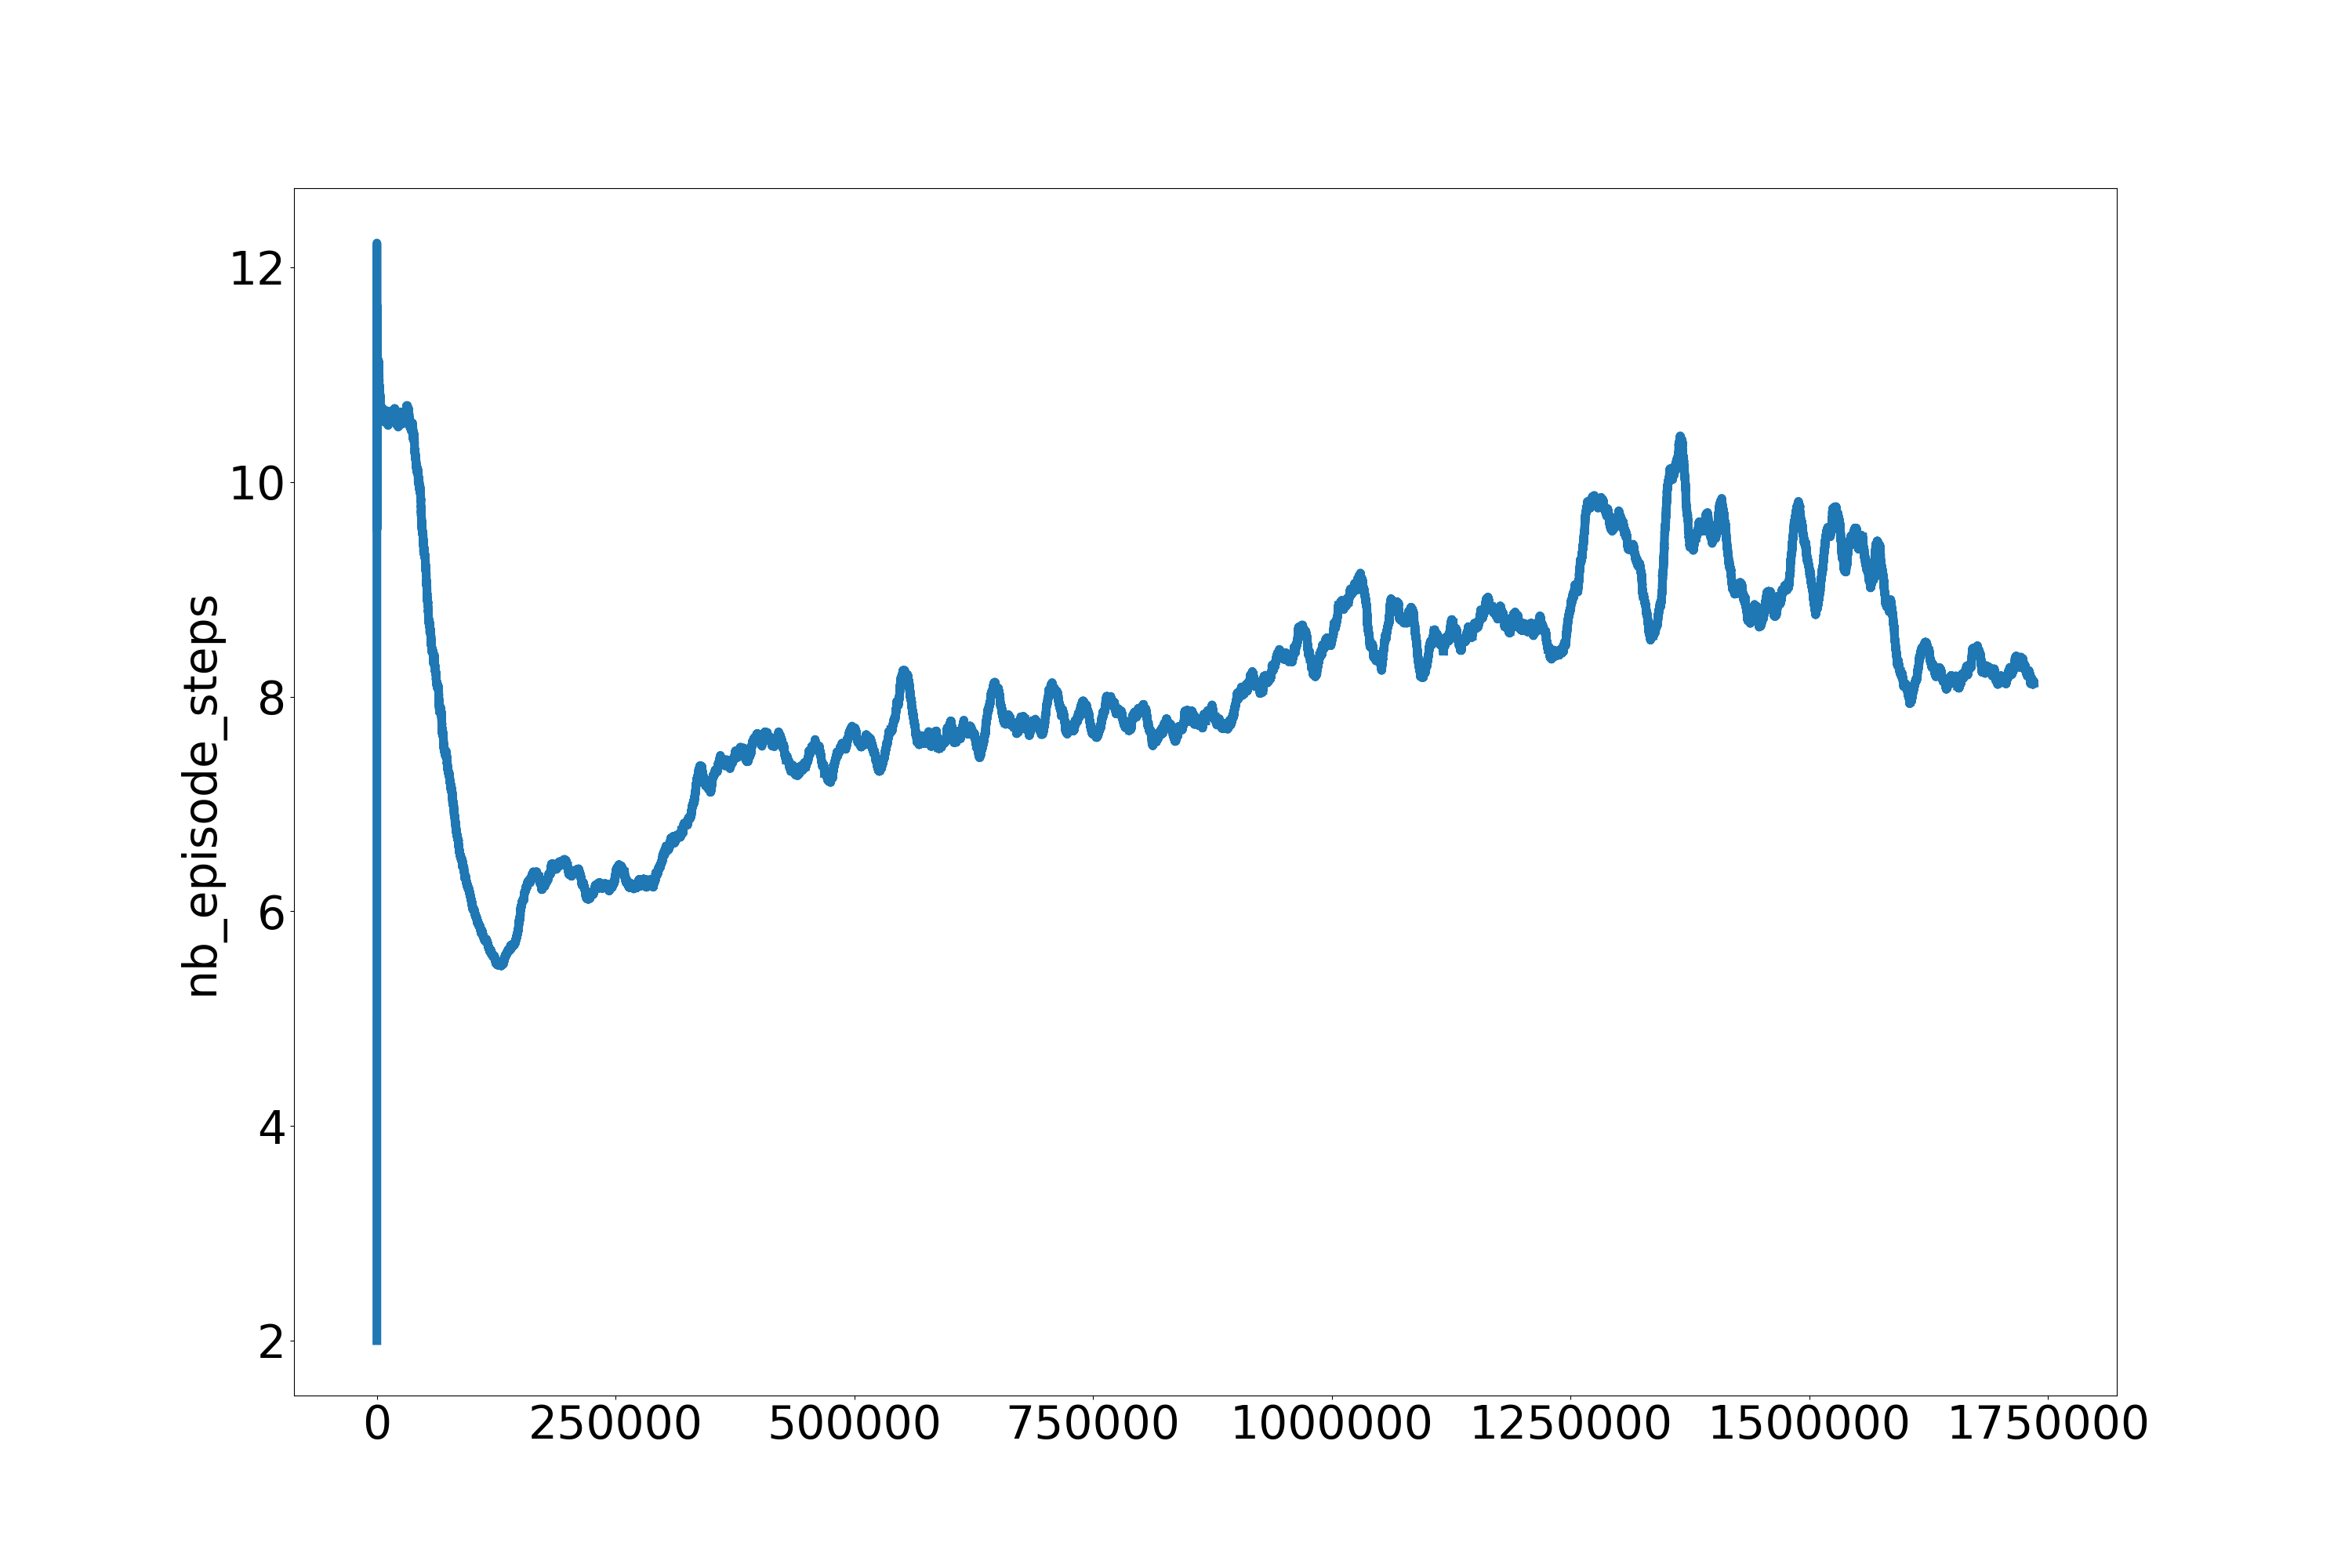
\includegraphics[width=0.85\textwidth]{Pic/First_model/nb_episode_steps.png}
    		\caption{Số bước thực hiện}
    		\label{fig:baseline_step}
    	\end{subfigure}%
    	\begin{subfigure}{.5\textwidth}
    		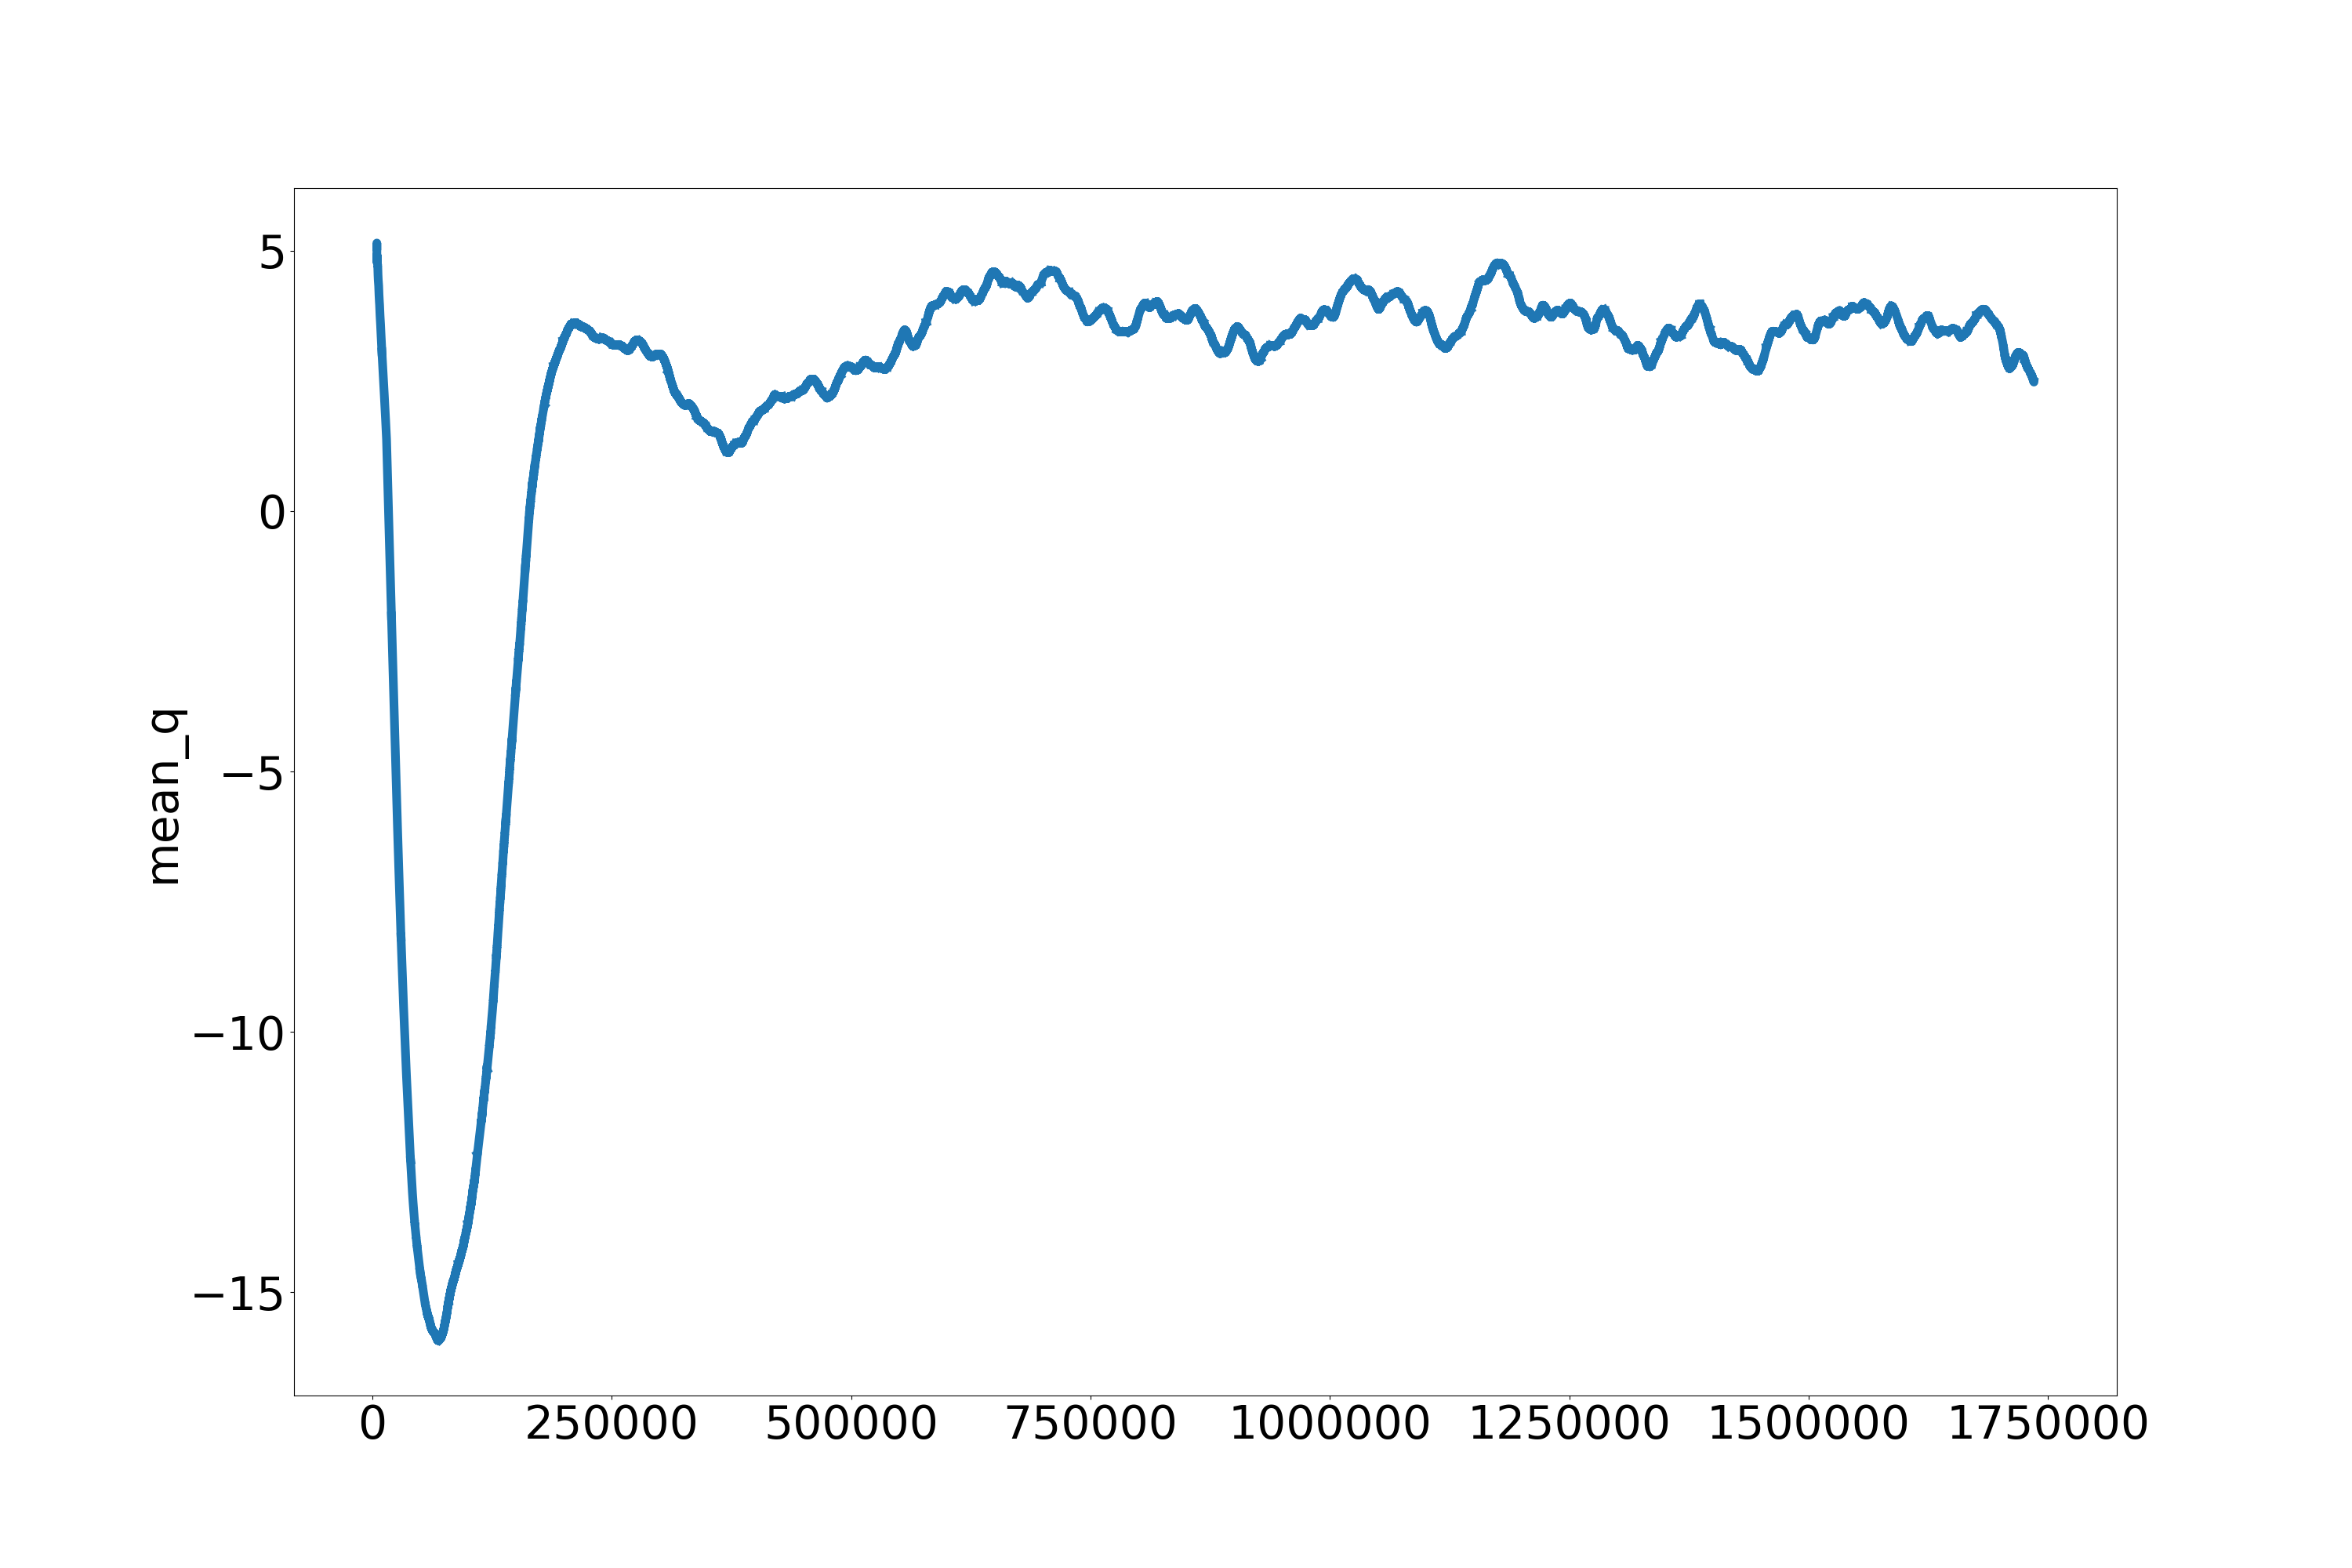
\includegraphics[width=0.85\textwidth]{Pic/First_model/mean_q.png}
    		\caption{Trung bình giá trị Q}
    		\label{fig:baseline_mean_q}
    	\end{subfigure}
    	\label{fig:result_baseline}
    \end{figure}
\end{frame}
%---------------------------------------------------------------%
\begin{frame}{Mô hình thứ nhất}
Lần 2\\
    \begin{subnumcases}{r(s_t,a_t,s_{t+1})=}
        +50 & $s_{t+1}=\text{đích}$\nonumber \\
        -50 & $s_{t+1}=\text{chết}$\nonumber\\
        -d(s_{t+1}) & còn lại\nonumber
    \end{subnumcases}
    Với
    \[d(s_{t+1}) = \frac{\text{vị trí cột đích}-\text{vị trí cột trạng thái tiếp theo}}{(\text{\text{vị trí cột đích} - \text{vị trí cột bắt đầu}})\times10}\]
\end{frame}
%---------------------------------------------------------------%
\begin{frame}{Mô hình thứ nhất}
Lần 2
\begin{figure}[ht]
    	\centering
    	\begin{subfigure}{.5\textwidth}
    		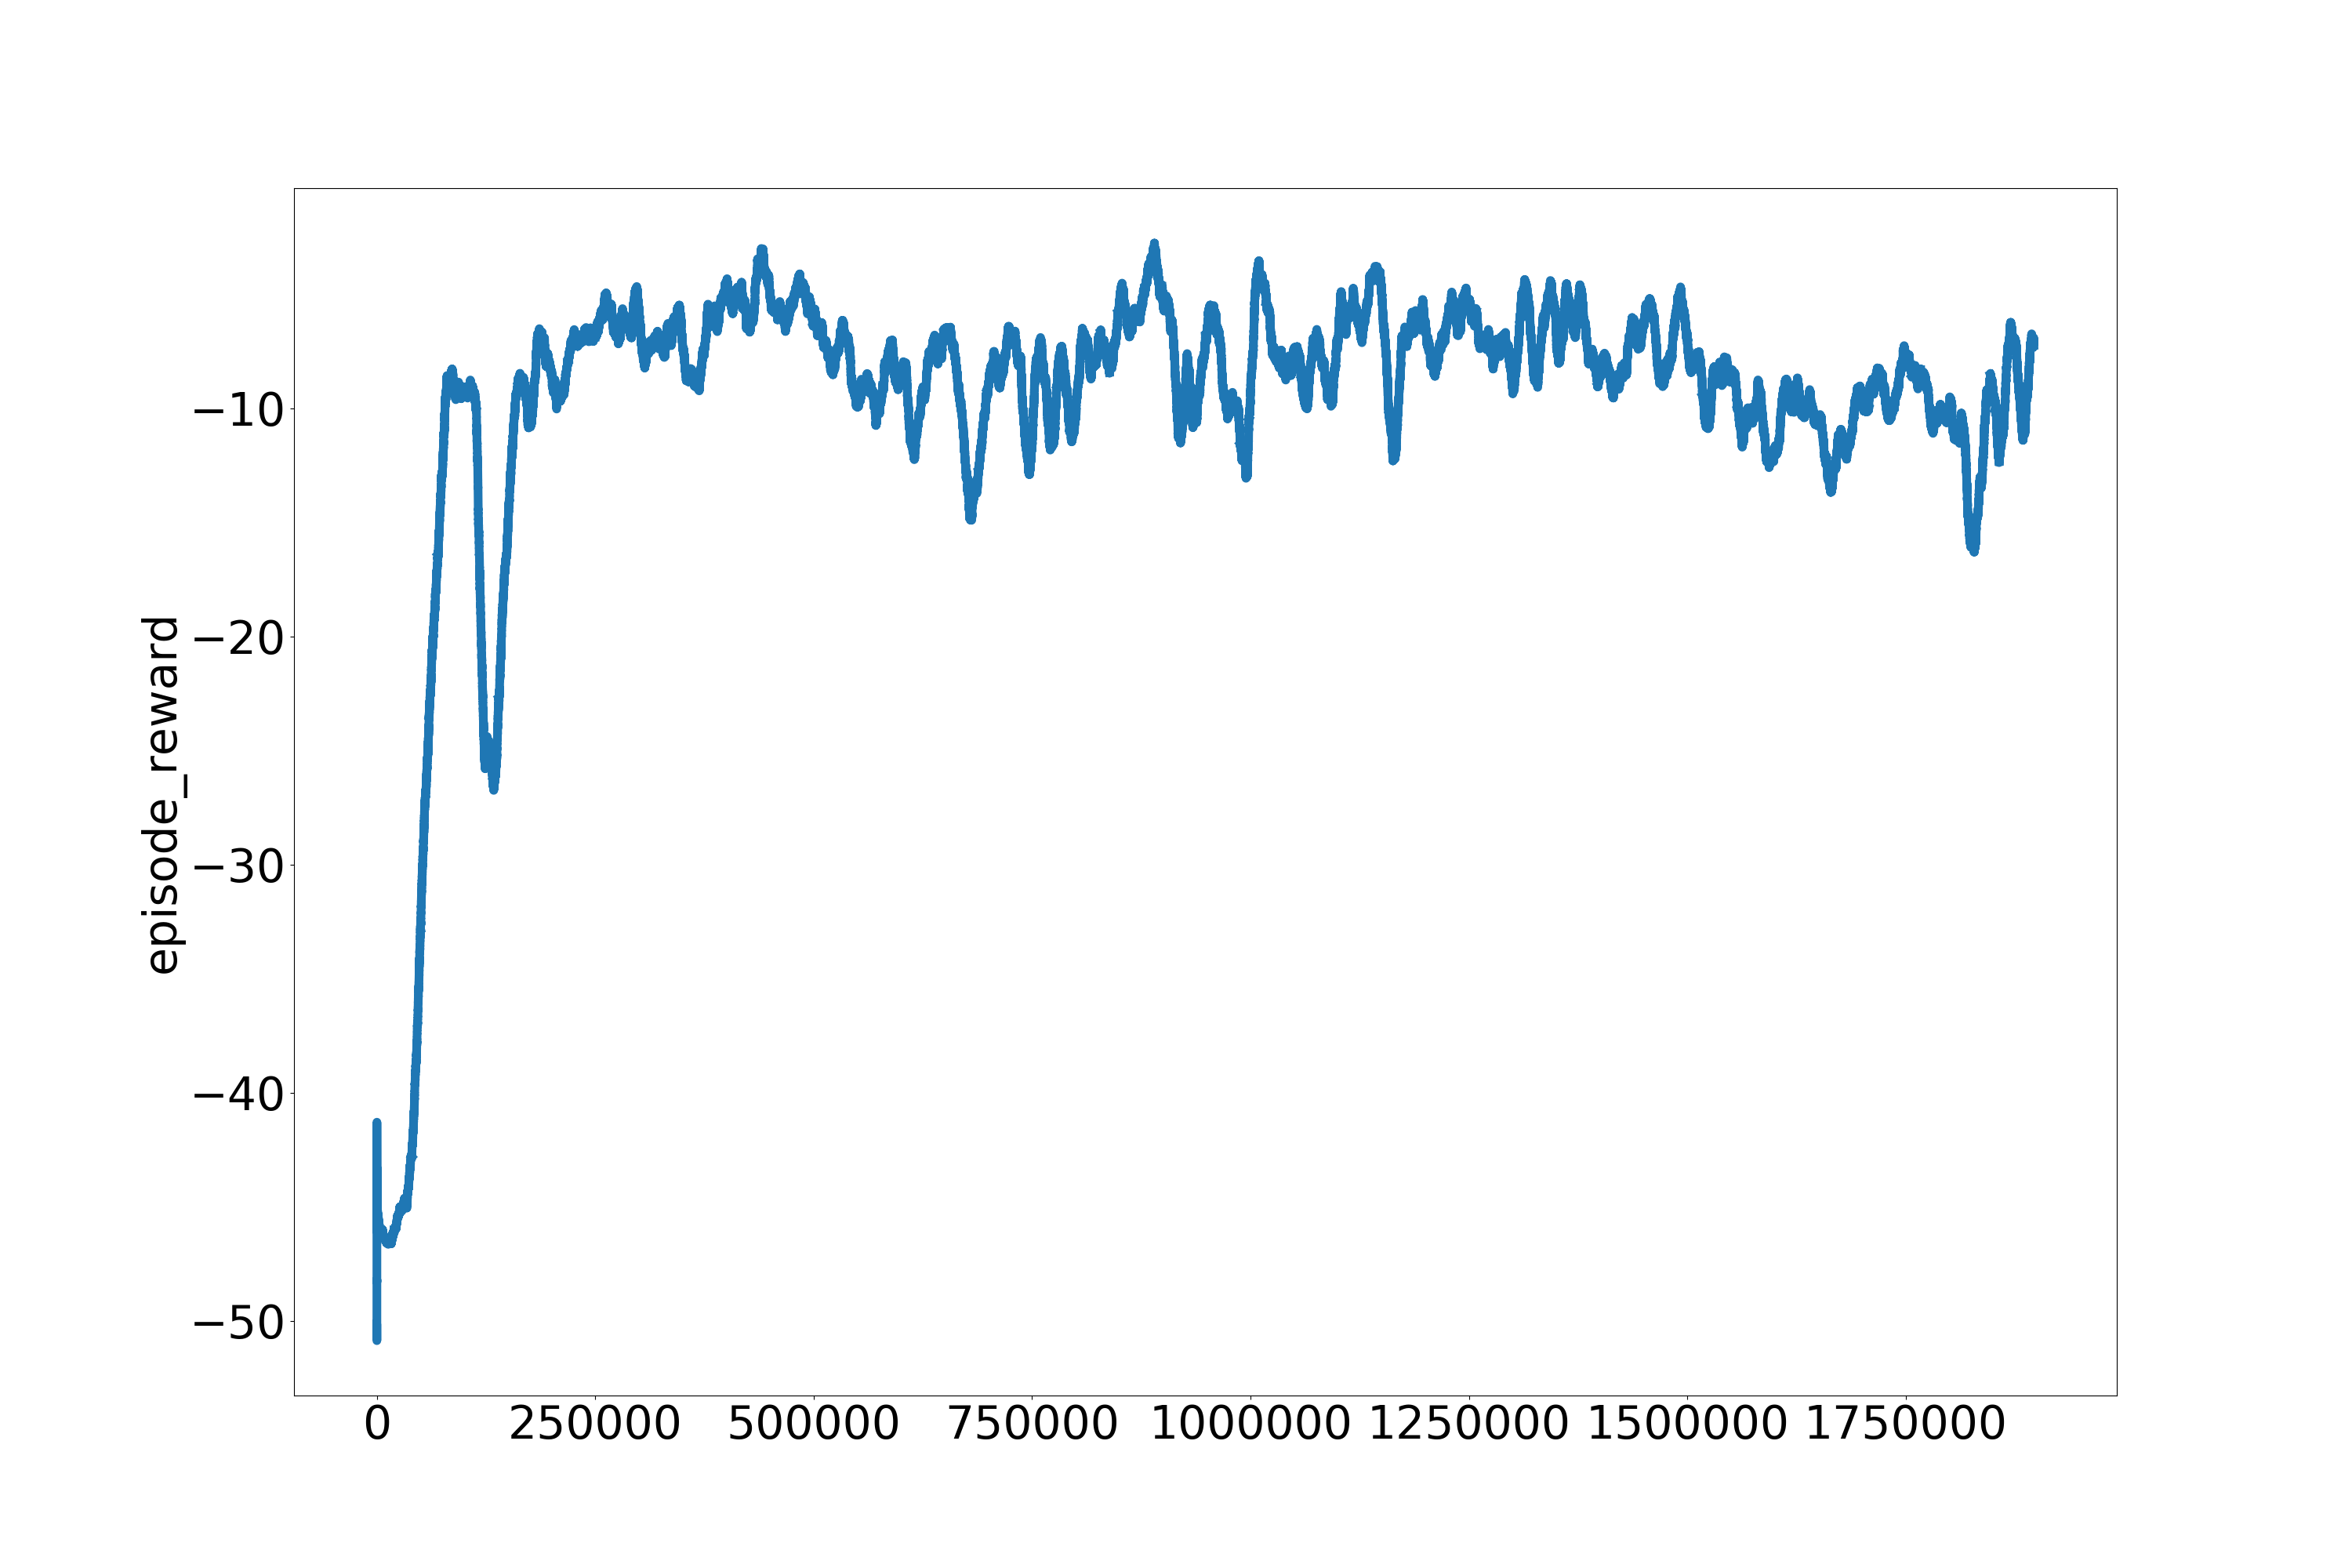
\includegraphics[width=0.85\textwidth]{Pic/First_model_50_reward/episode_reward.png}
    		\caption{Trung bình tích lũy phần thưởng}
    		\label{fig:baseline_avg}
    	\end{subfigure}%
    	\begin{subfigure}{.5\textwidth}
    		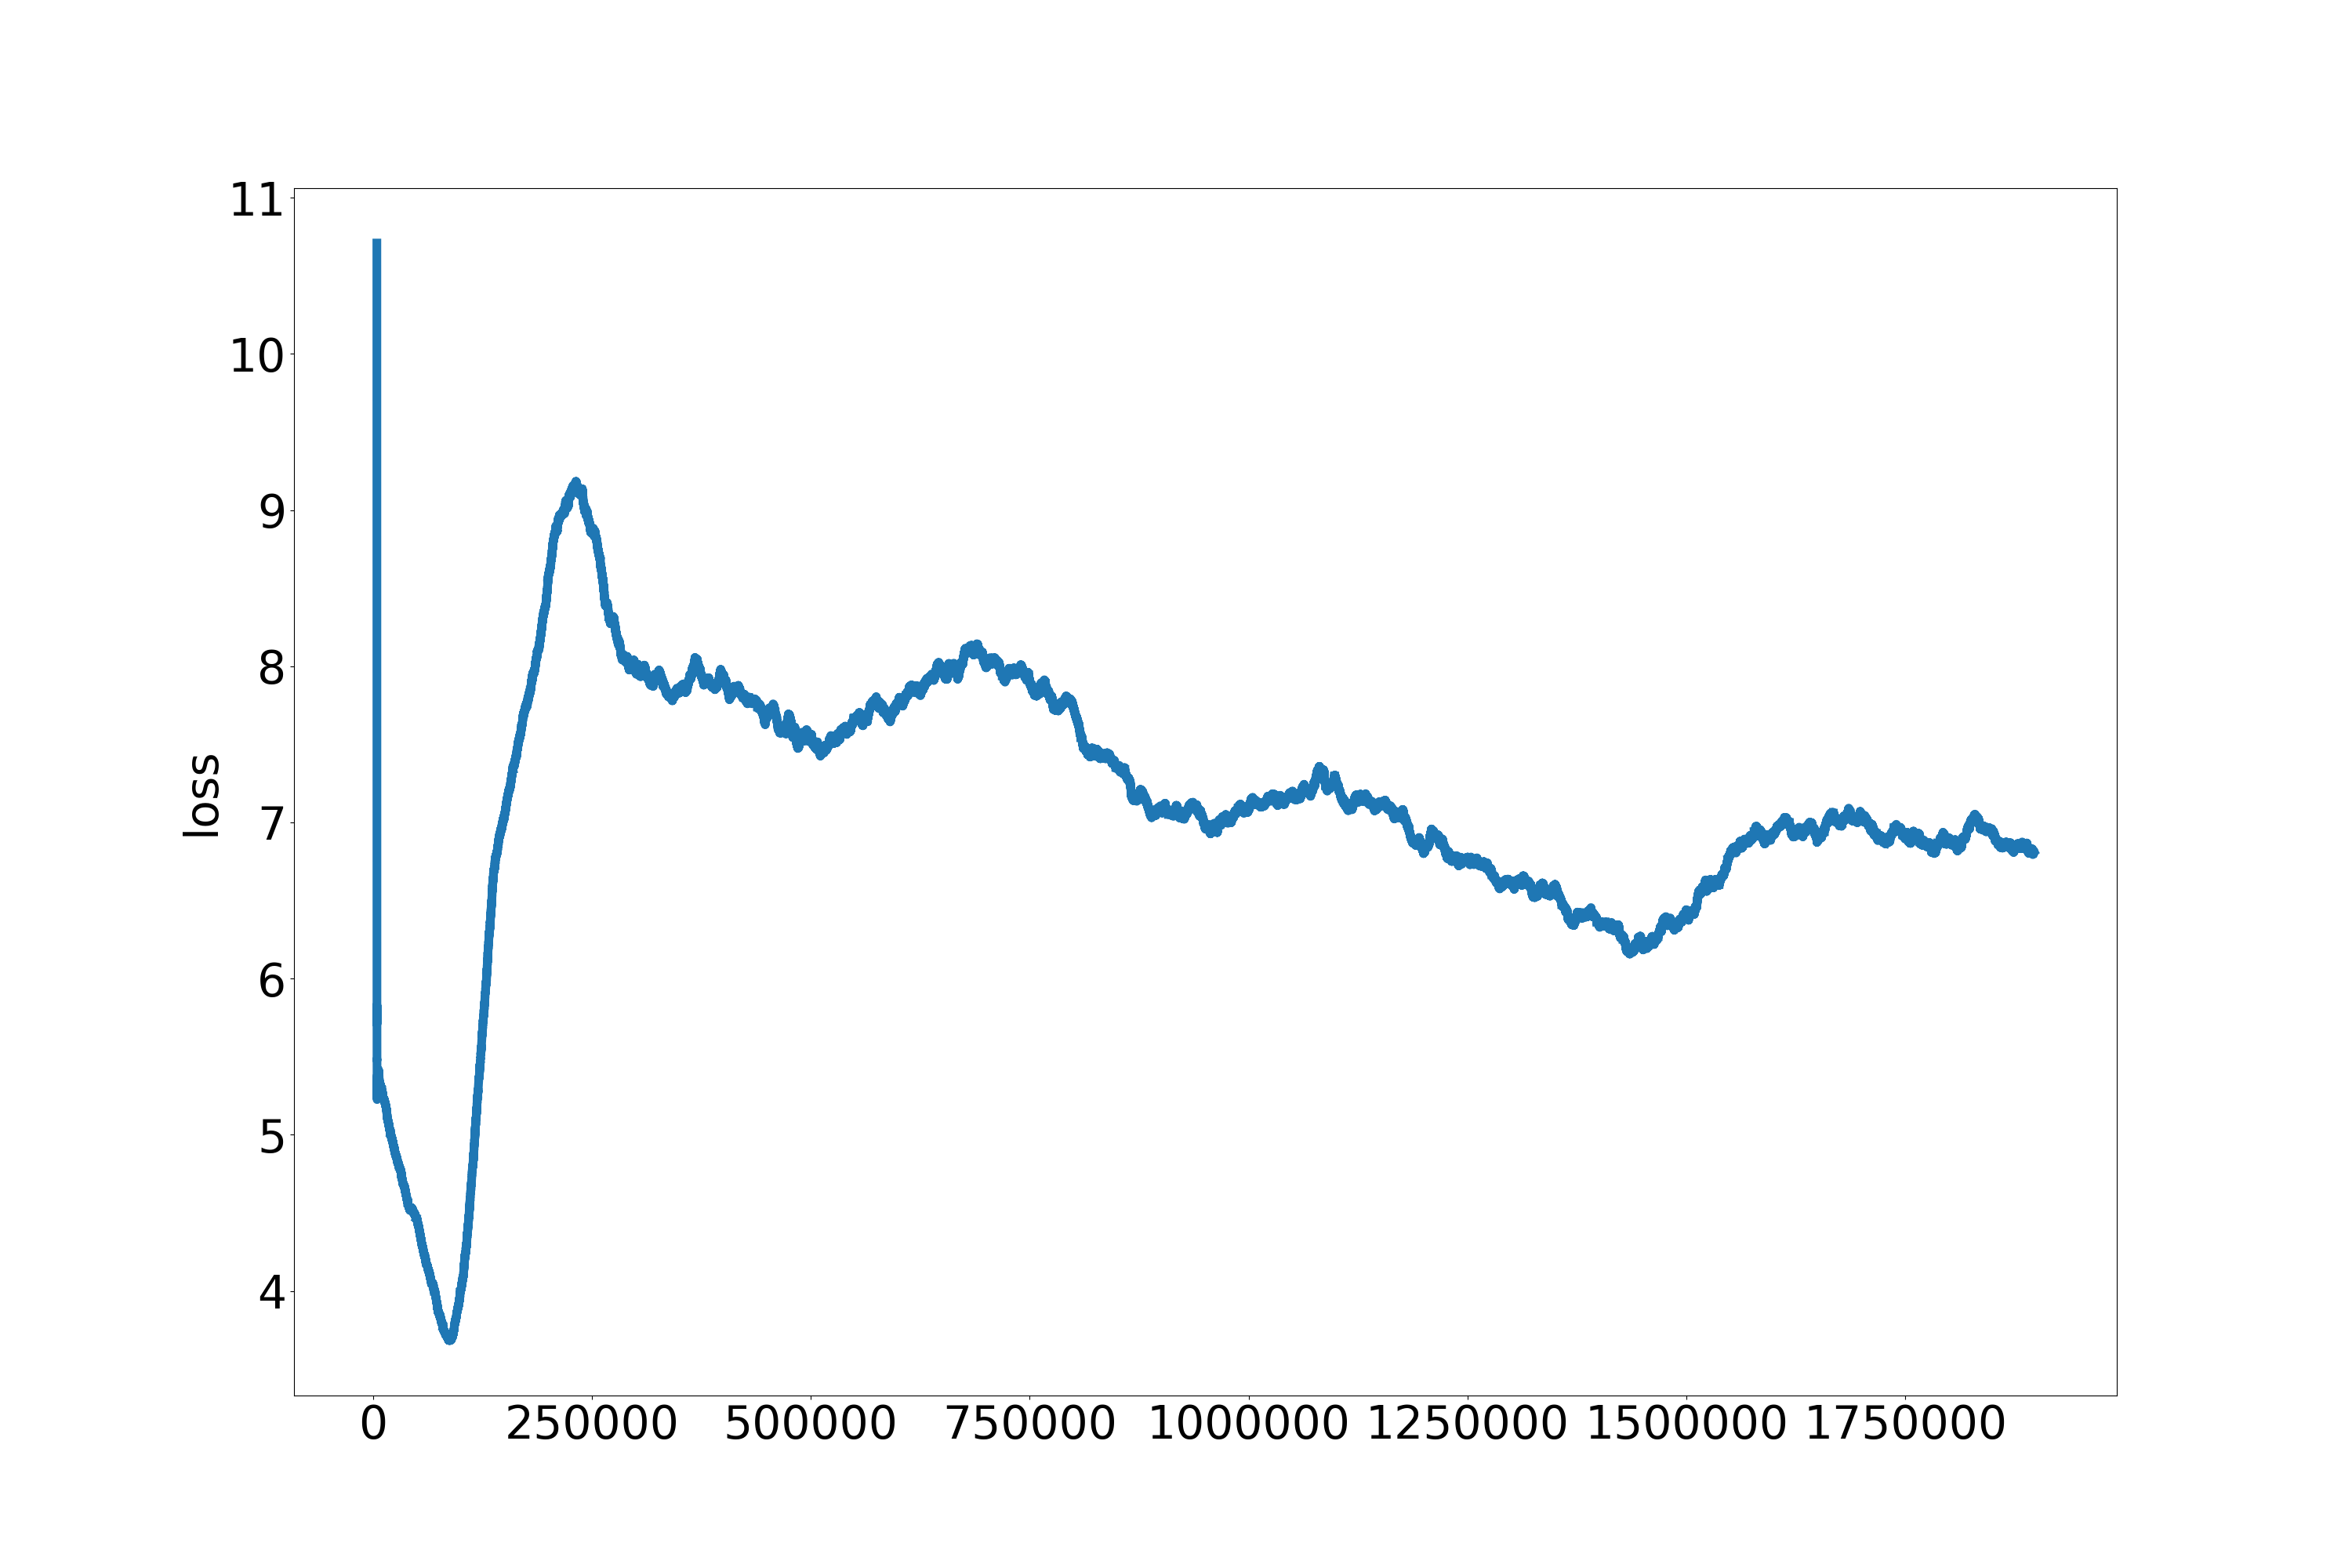
\includegraphics[width=0.85\textwidth]{Pic/First_model_50_reward/loss.png}
    		\caption{Hàm mất mát}
    		\label{fig:baseline_loss}
    	\end{subfigure}\\
    	\begin{subfigure}{.5\textwidth}
    		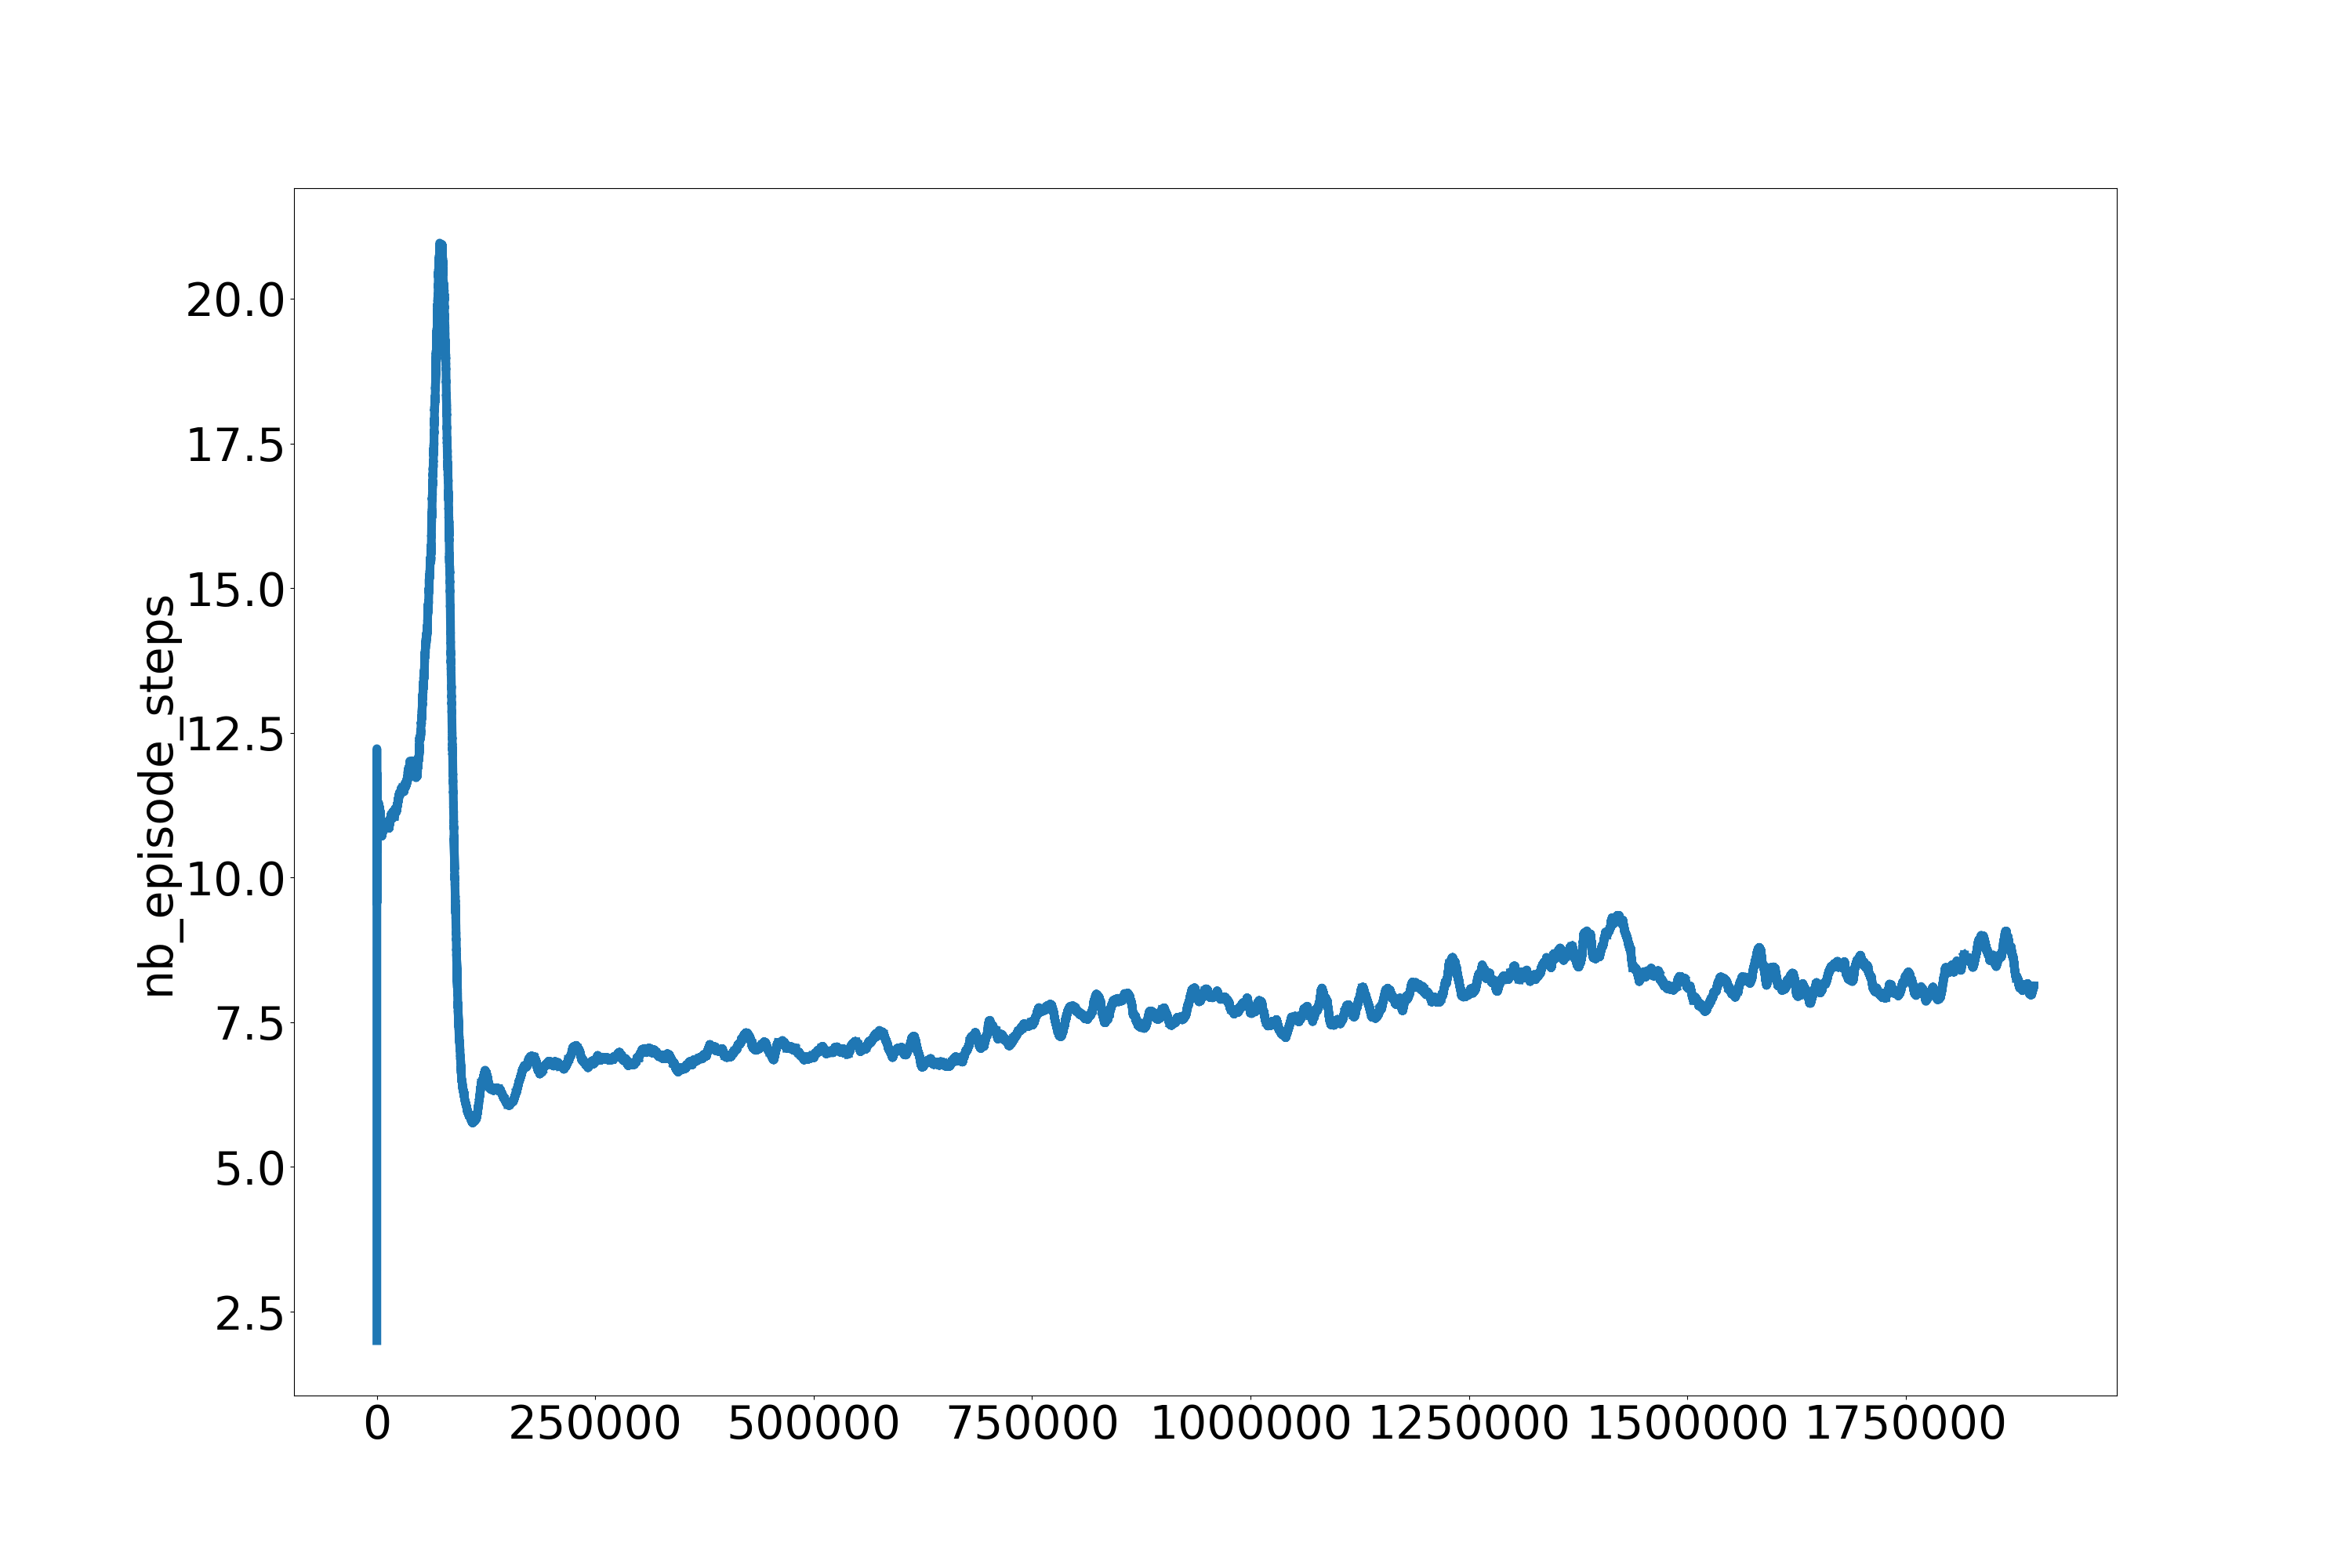
\includegraphics[width=0.85\textwidth]{Pic/First_model_50_reward/nb_episode_steps.png}
    		\caption{Số bước thực hiện}
    		\label{fig:baseline_step}
    	\end{subfigure}%
    	\begin{subfigure}{.5\textwidth}
    		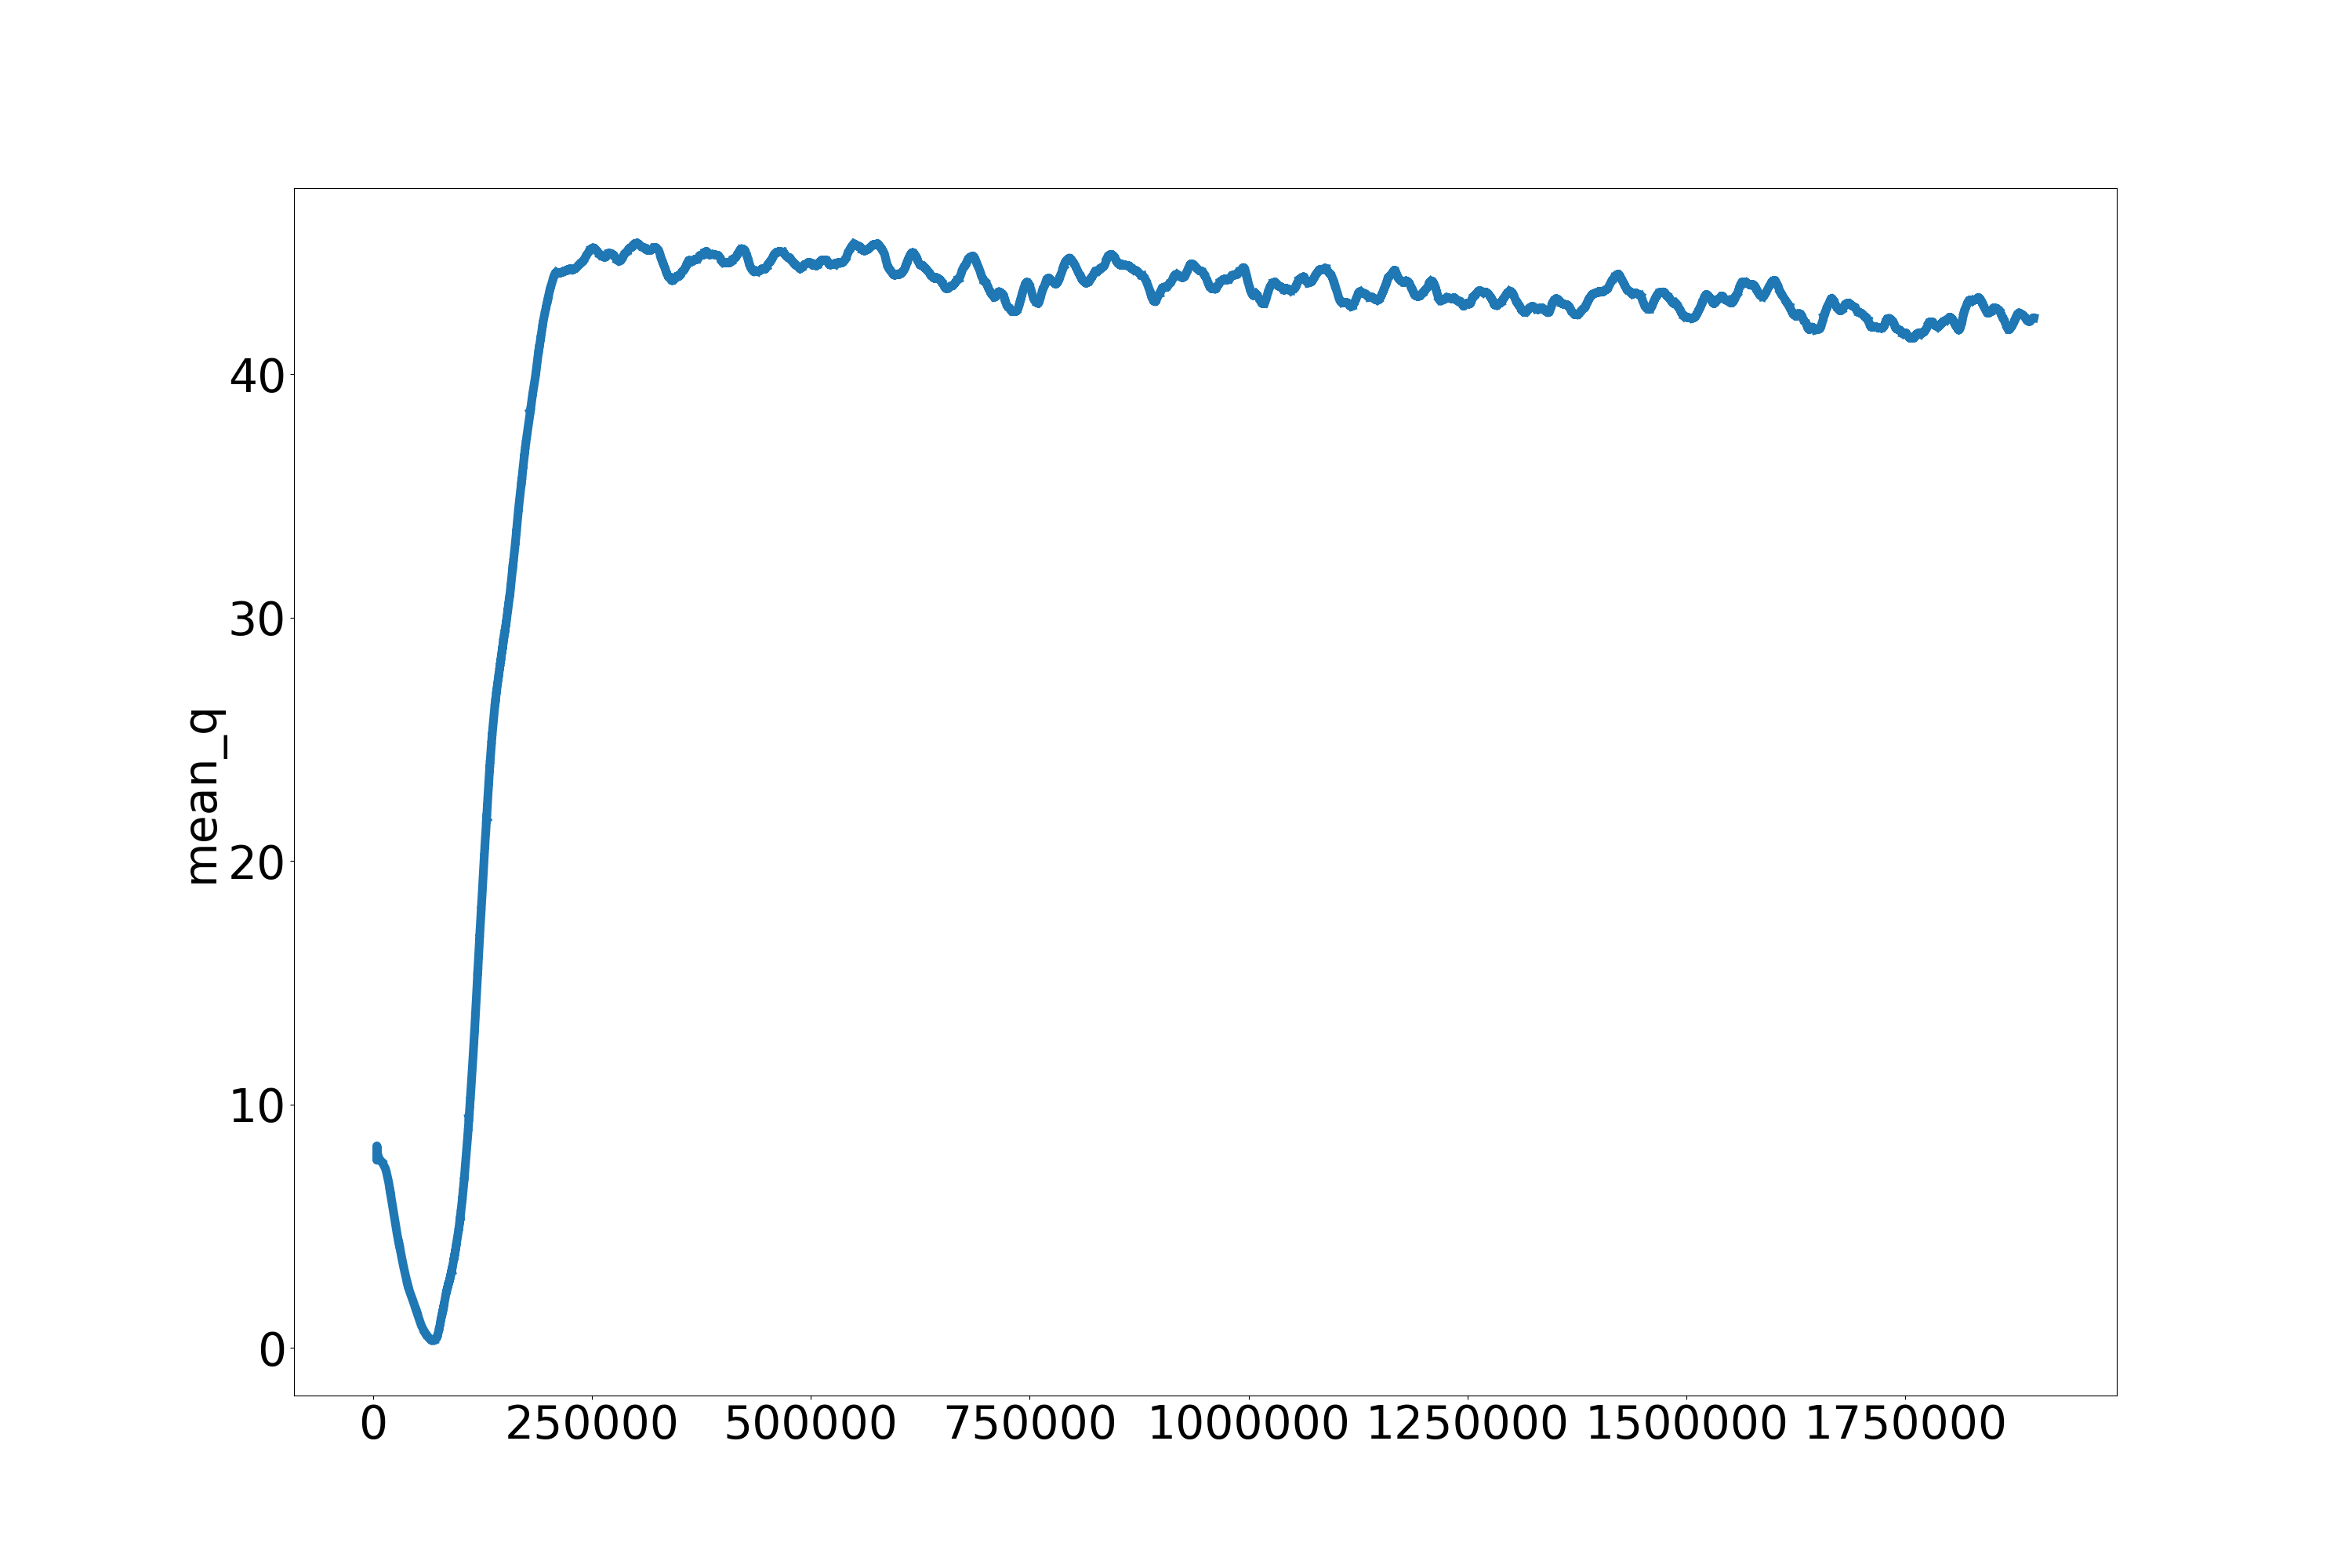
\includegraphics[width=0.85\textwidth]{Pic/First_model_50_reward/mean_q.png}
    		\caption{Trung bình giá trị Q}
    		\label{fig:baseline_mean_q}
    	\end{subfigure}
    	\label{fig:result_baseline}
    \end{figure}
\end{frame}
%---------------------------------------------------------------%
\begin{frame}{Một số thử nghiệm}
    \textbf{Mô hình thứ hai}
    \vspace{0.5cm}
    \begin{itemize}
        \item 1.Thay đổi cấu trúc mô hình
        \vspace{0.5cm}
        \item 2. Thay đổi công cụ tối ưu
        \vspace{.5cm}
        \item 3. Thay đổi kích thước batch
    \end{itemize}
\end{frame}
%---------------------------------------------------------------%
\begin{frame}{Mô hình thứ hai}
	\begin{figure}
		\centering
		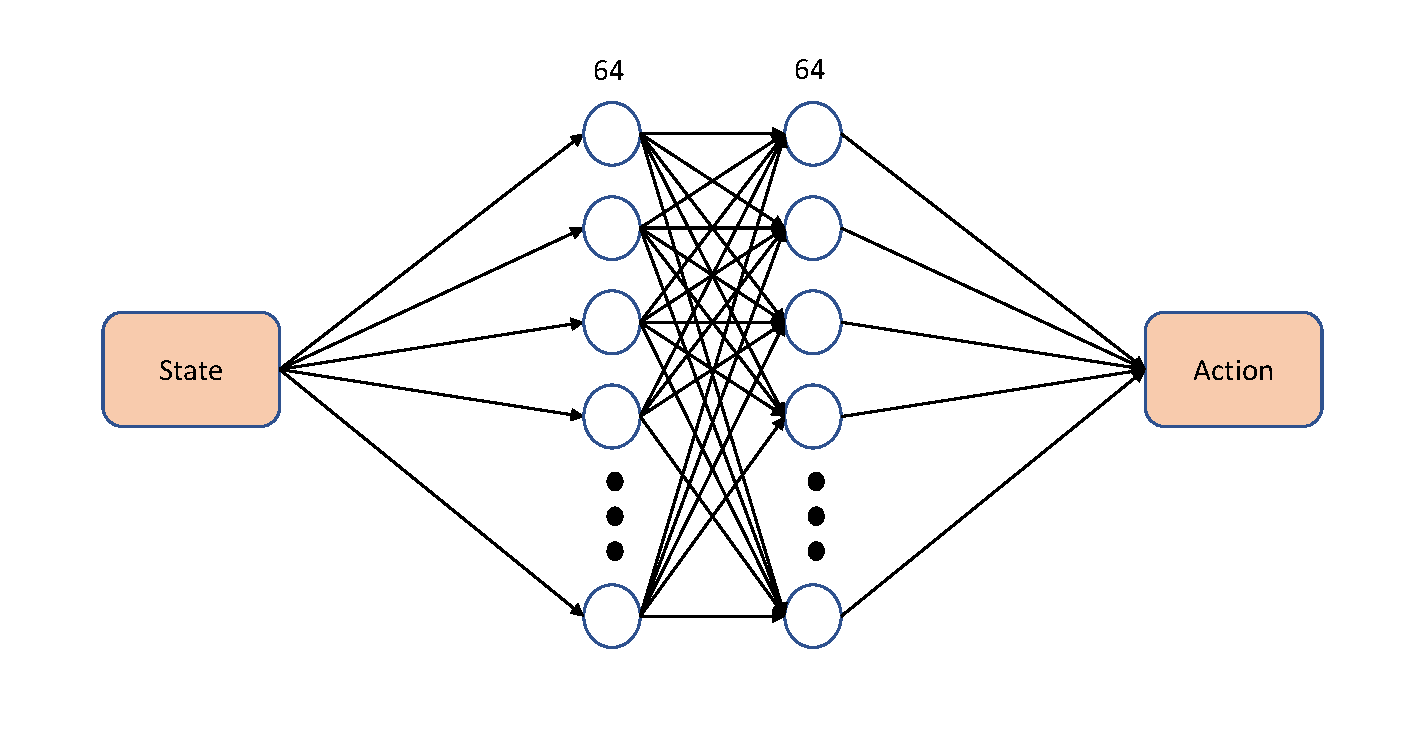
\includegraphics[width=\linewidth]{Pic/Second_model/second_arch.pdf}
	\end{figure}
\end{frame}
%---------------------------------------------------------------%
\begin{frame}{Mô hình thứ hai}
Tỷ lệ thắng 55,8\%.
\begin{figure}[ht]
    	\centering
    	\begin{subfigure}{.5\textwidth}
    		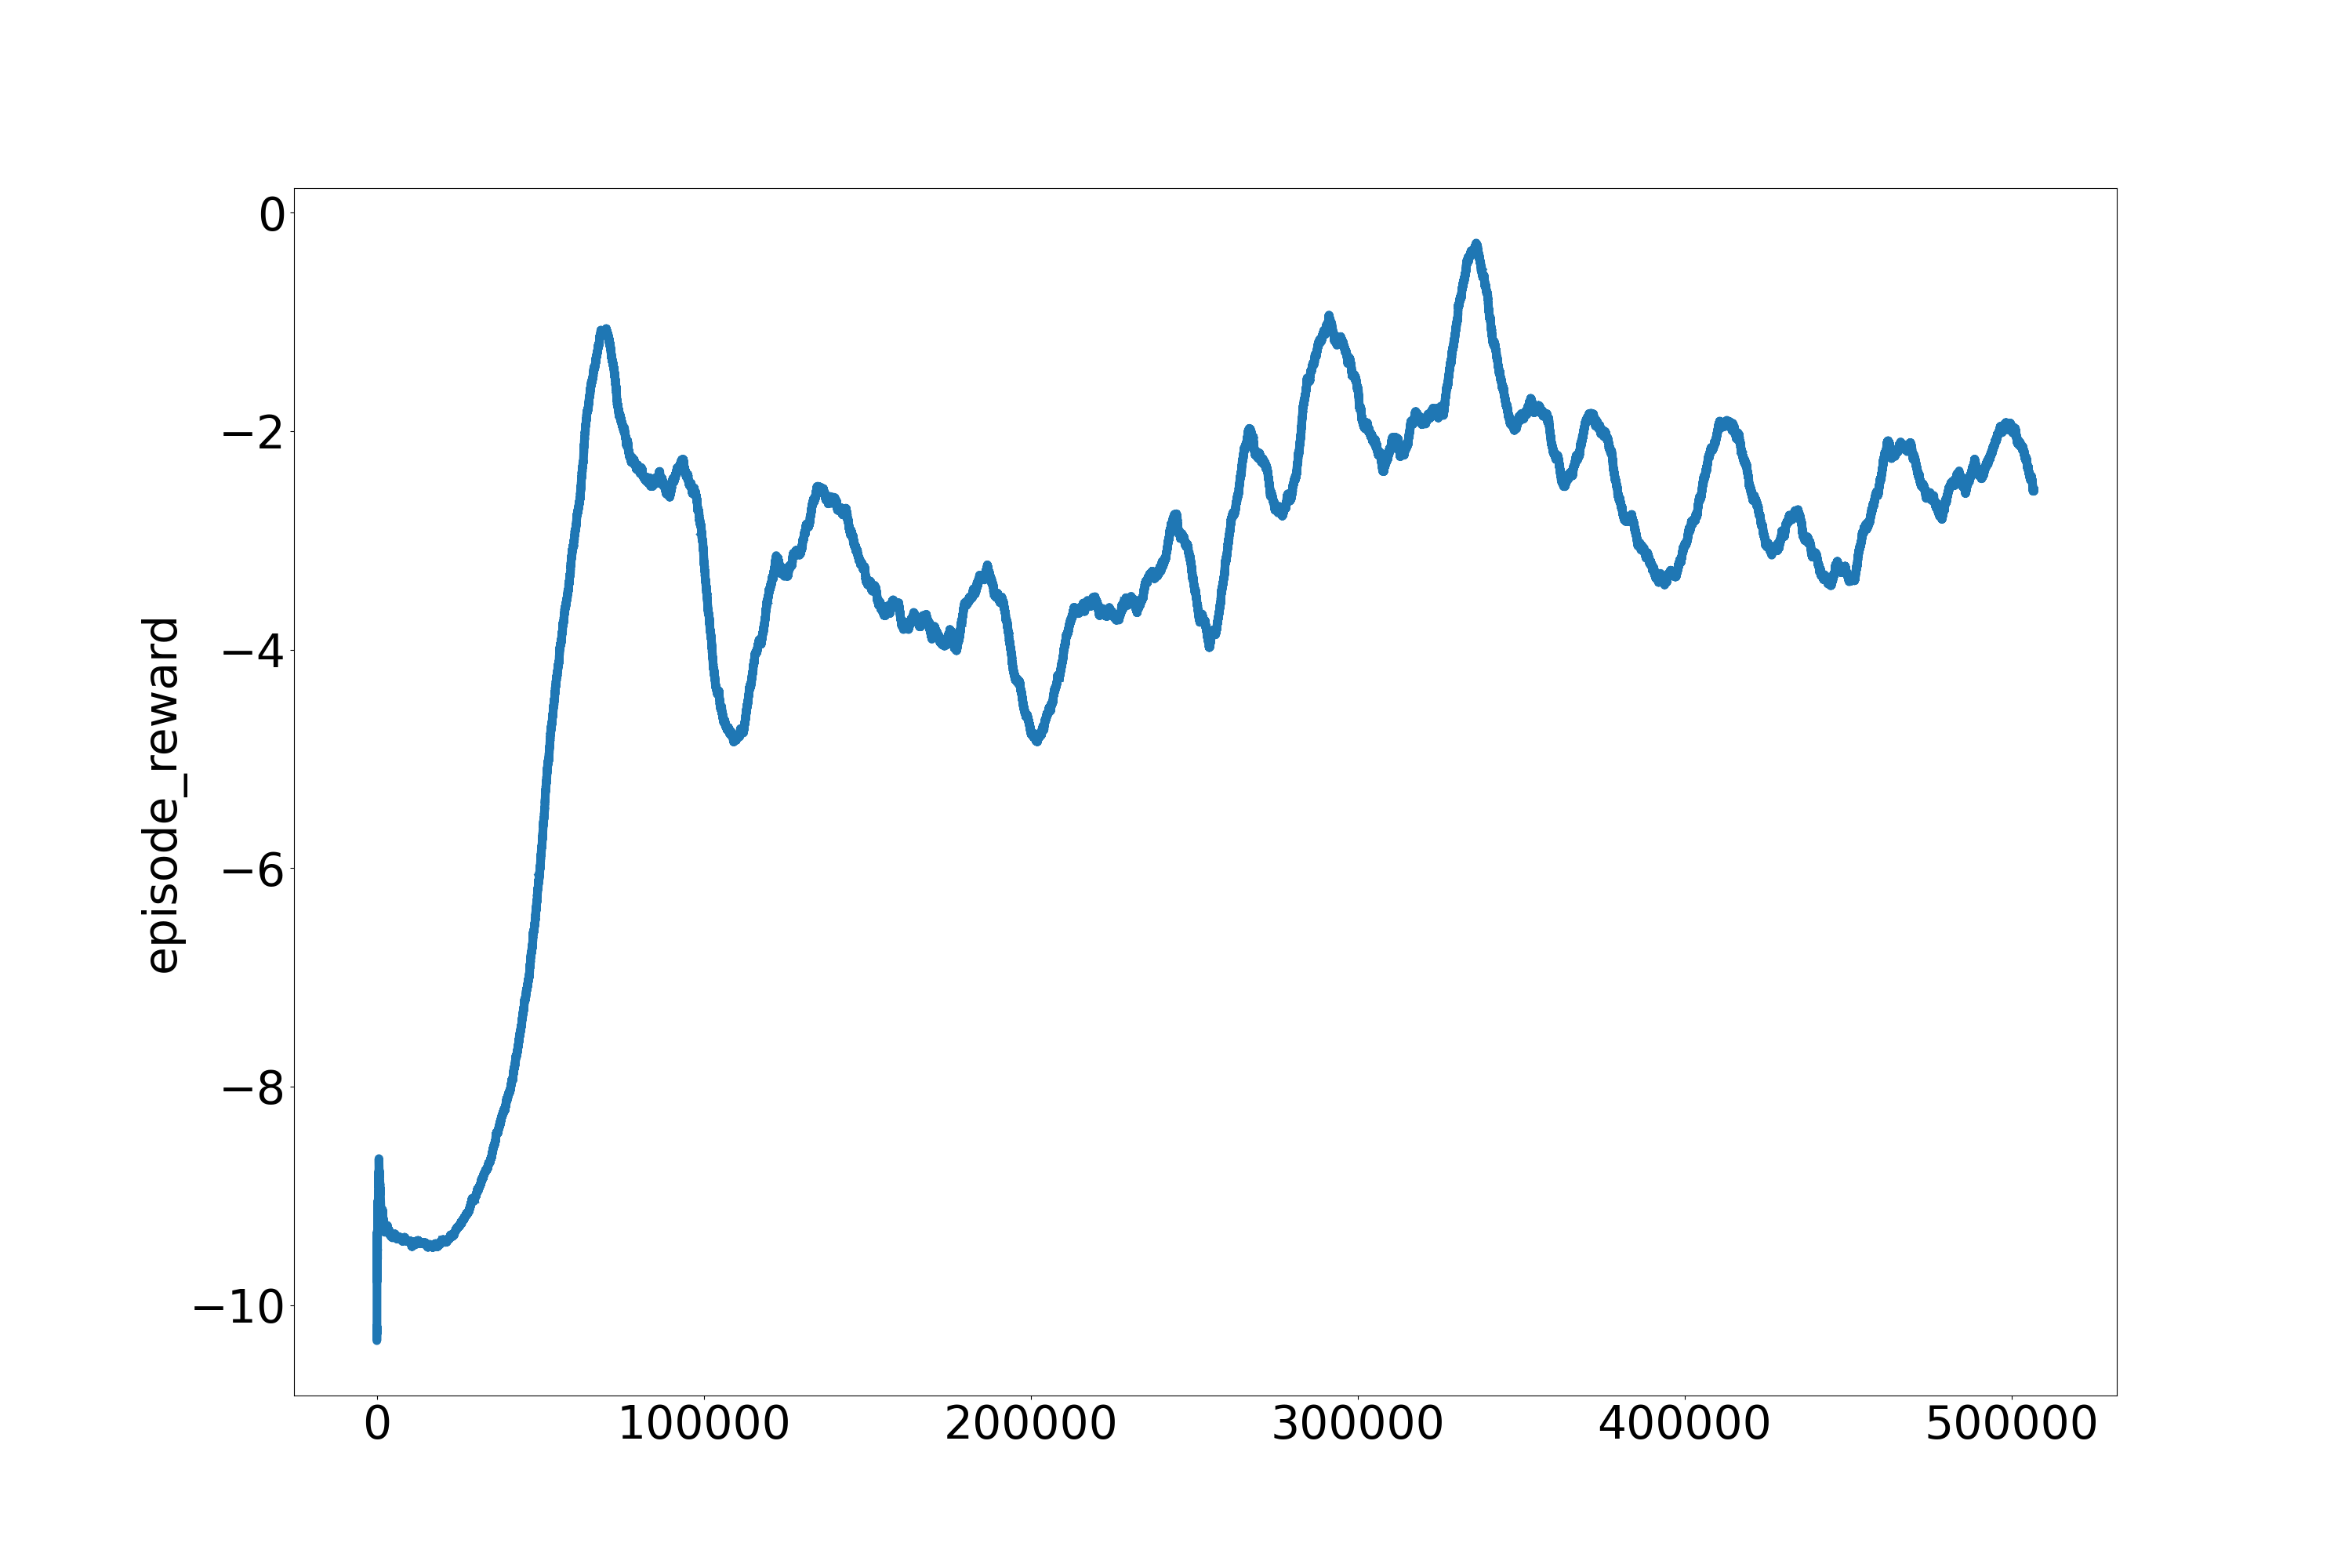
\includegraphics[width=0.85\textwidth]{Pic/Second_model/episode_reward.png}
    		\caption{Trung bình tích lũy phần thưởng}
    		\label{fig:baseline_avg}
    	\end{subfigure}%
    	\begin{subfigure}{.5\textwidth}
    		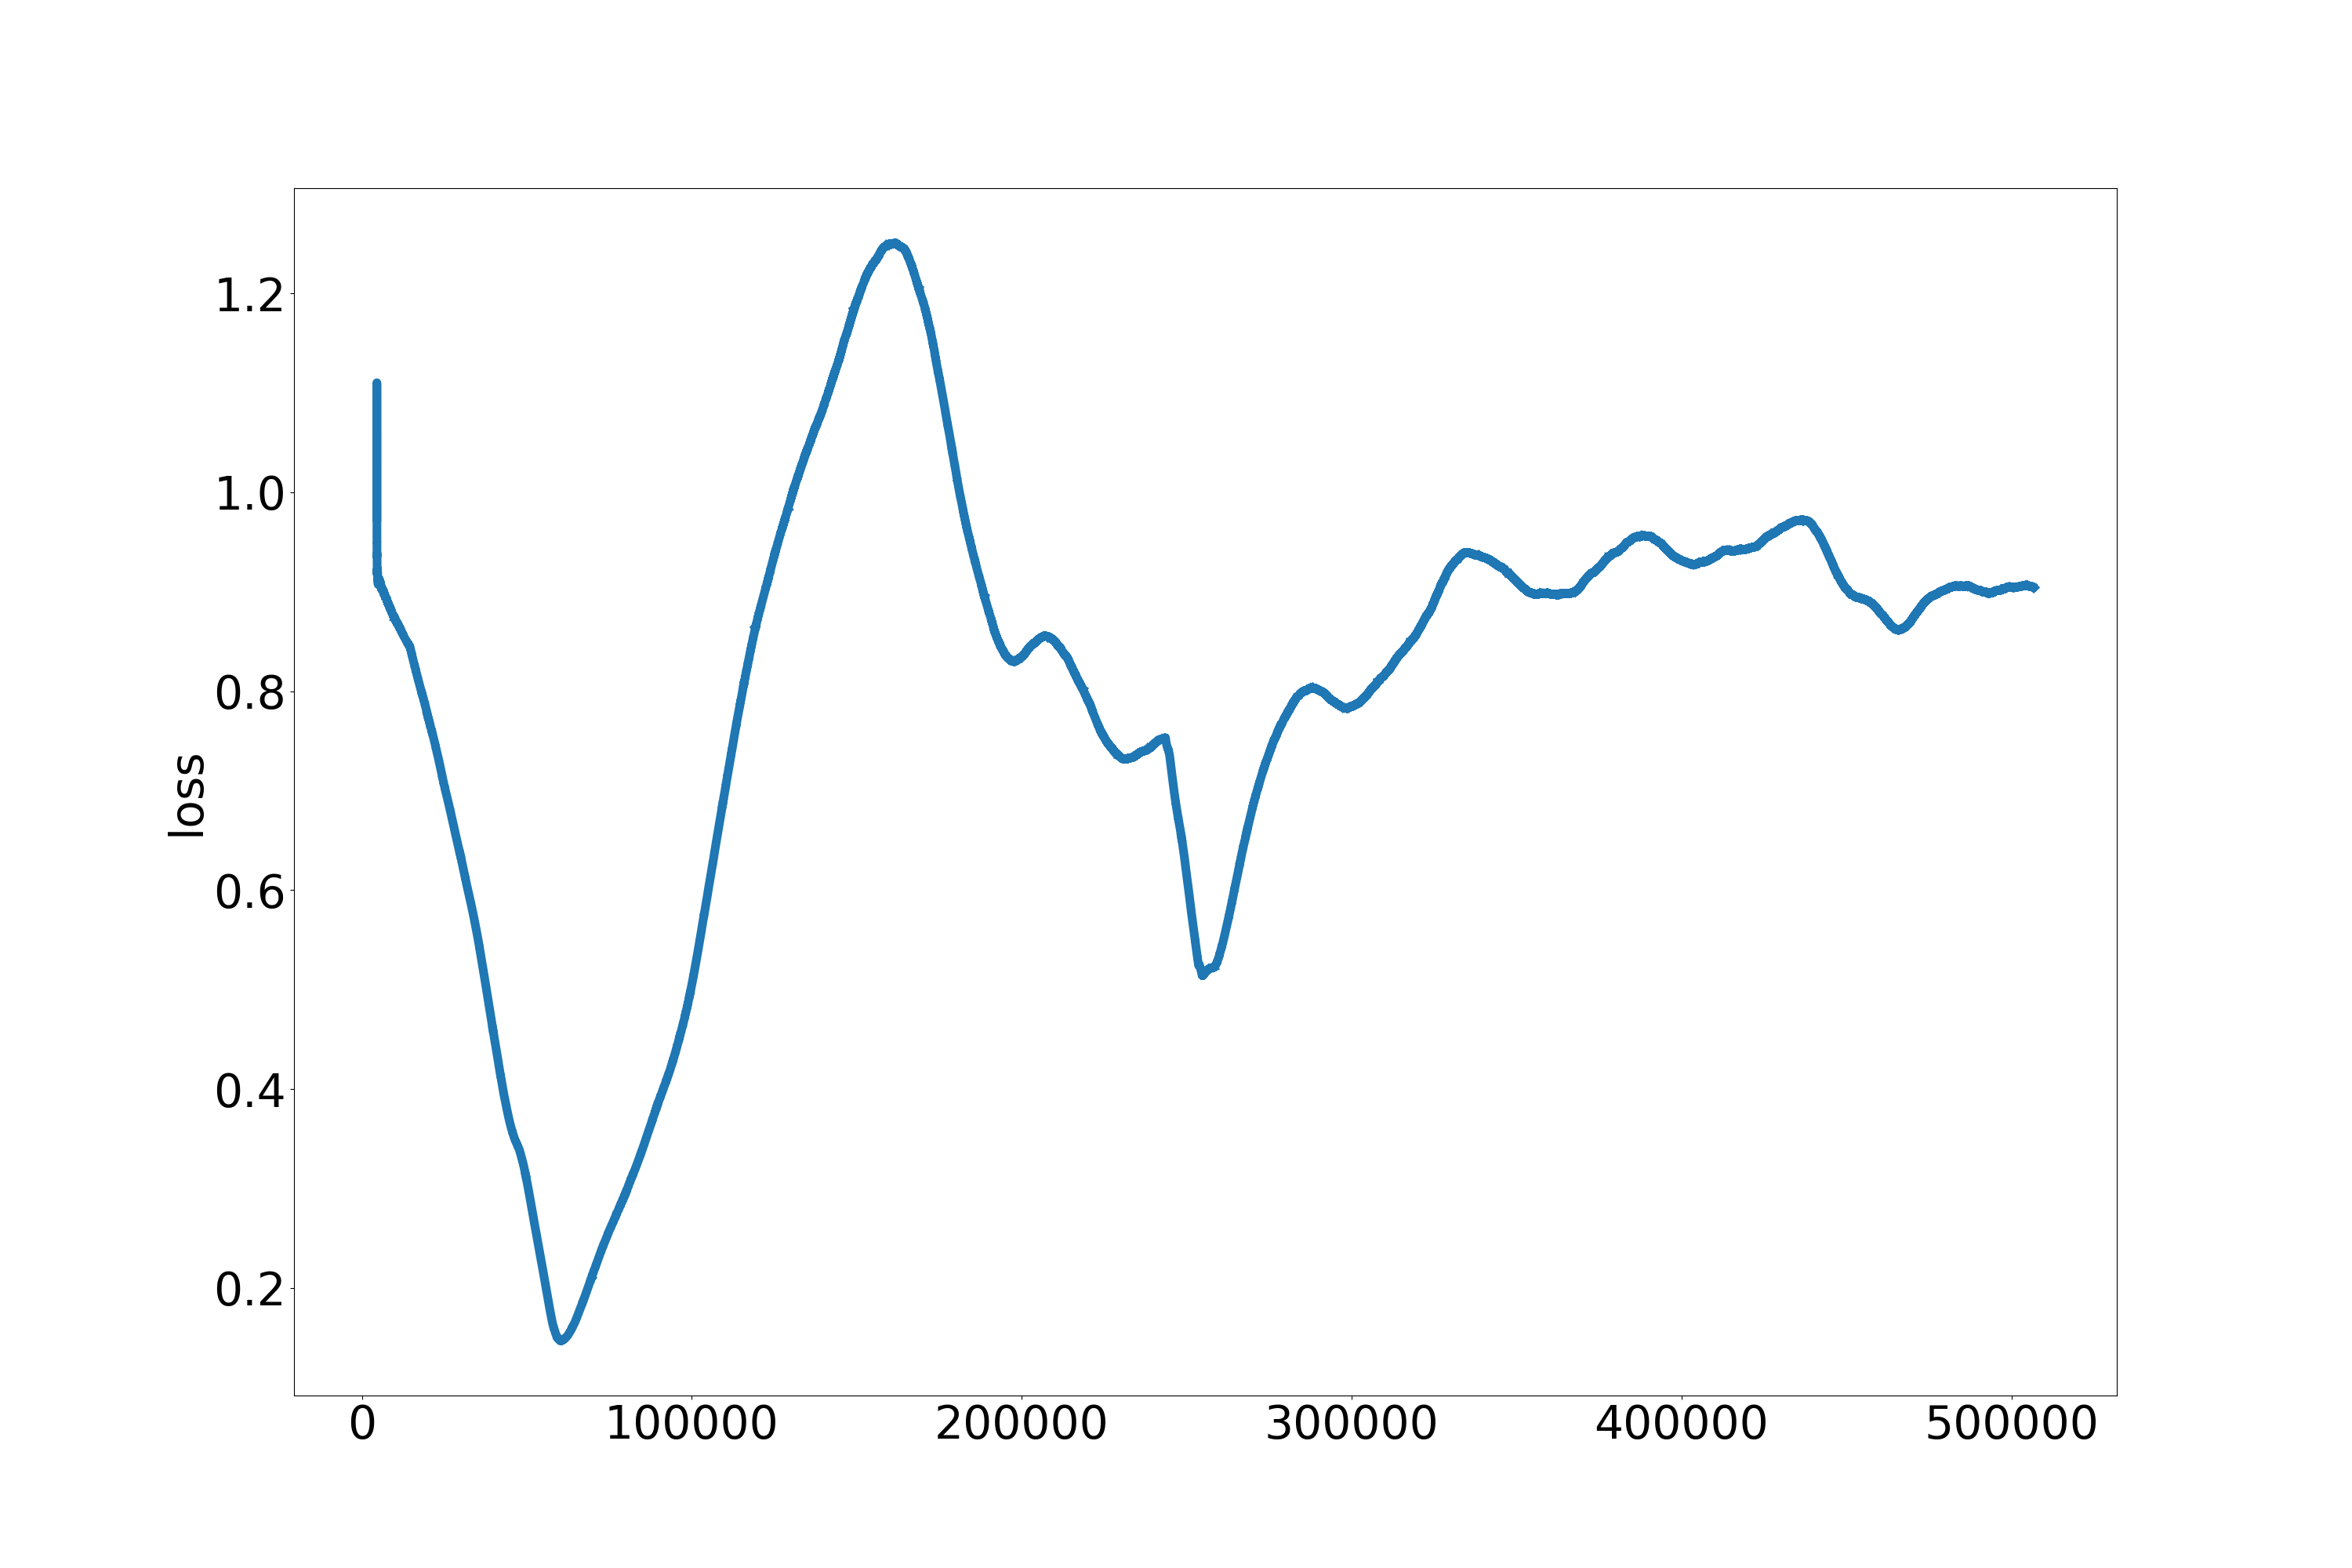
\includegraphics[width=0.85\textwidth]{Pic/Second_model/loss.png}
    		\caption{Hàm mất mát}
    		\label{fig:baseline_loss}
    	\end{subfigure}\\
    	\begin{subfigure}{.5\textwidth}
    		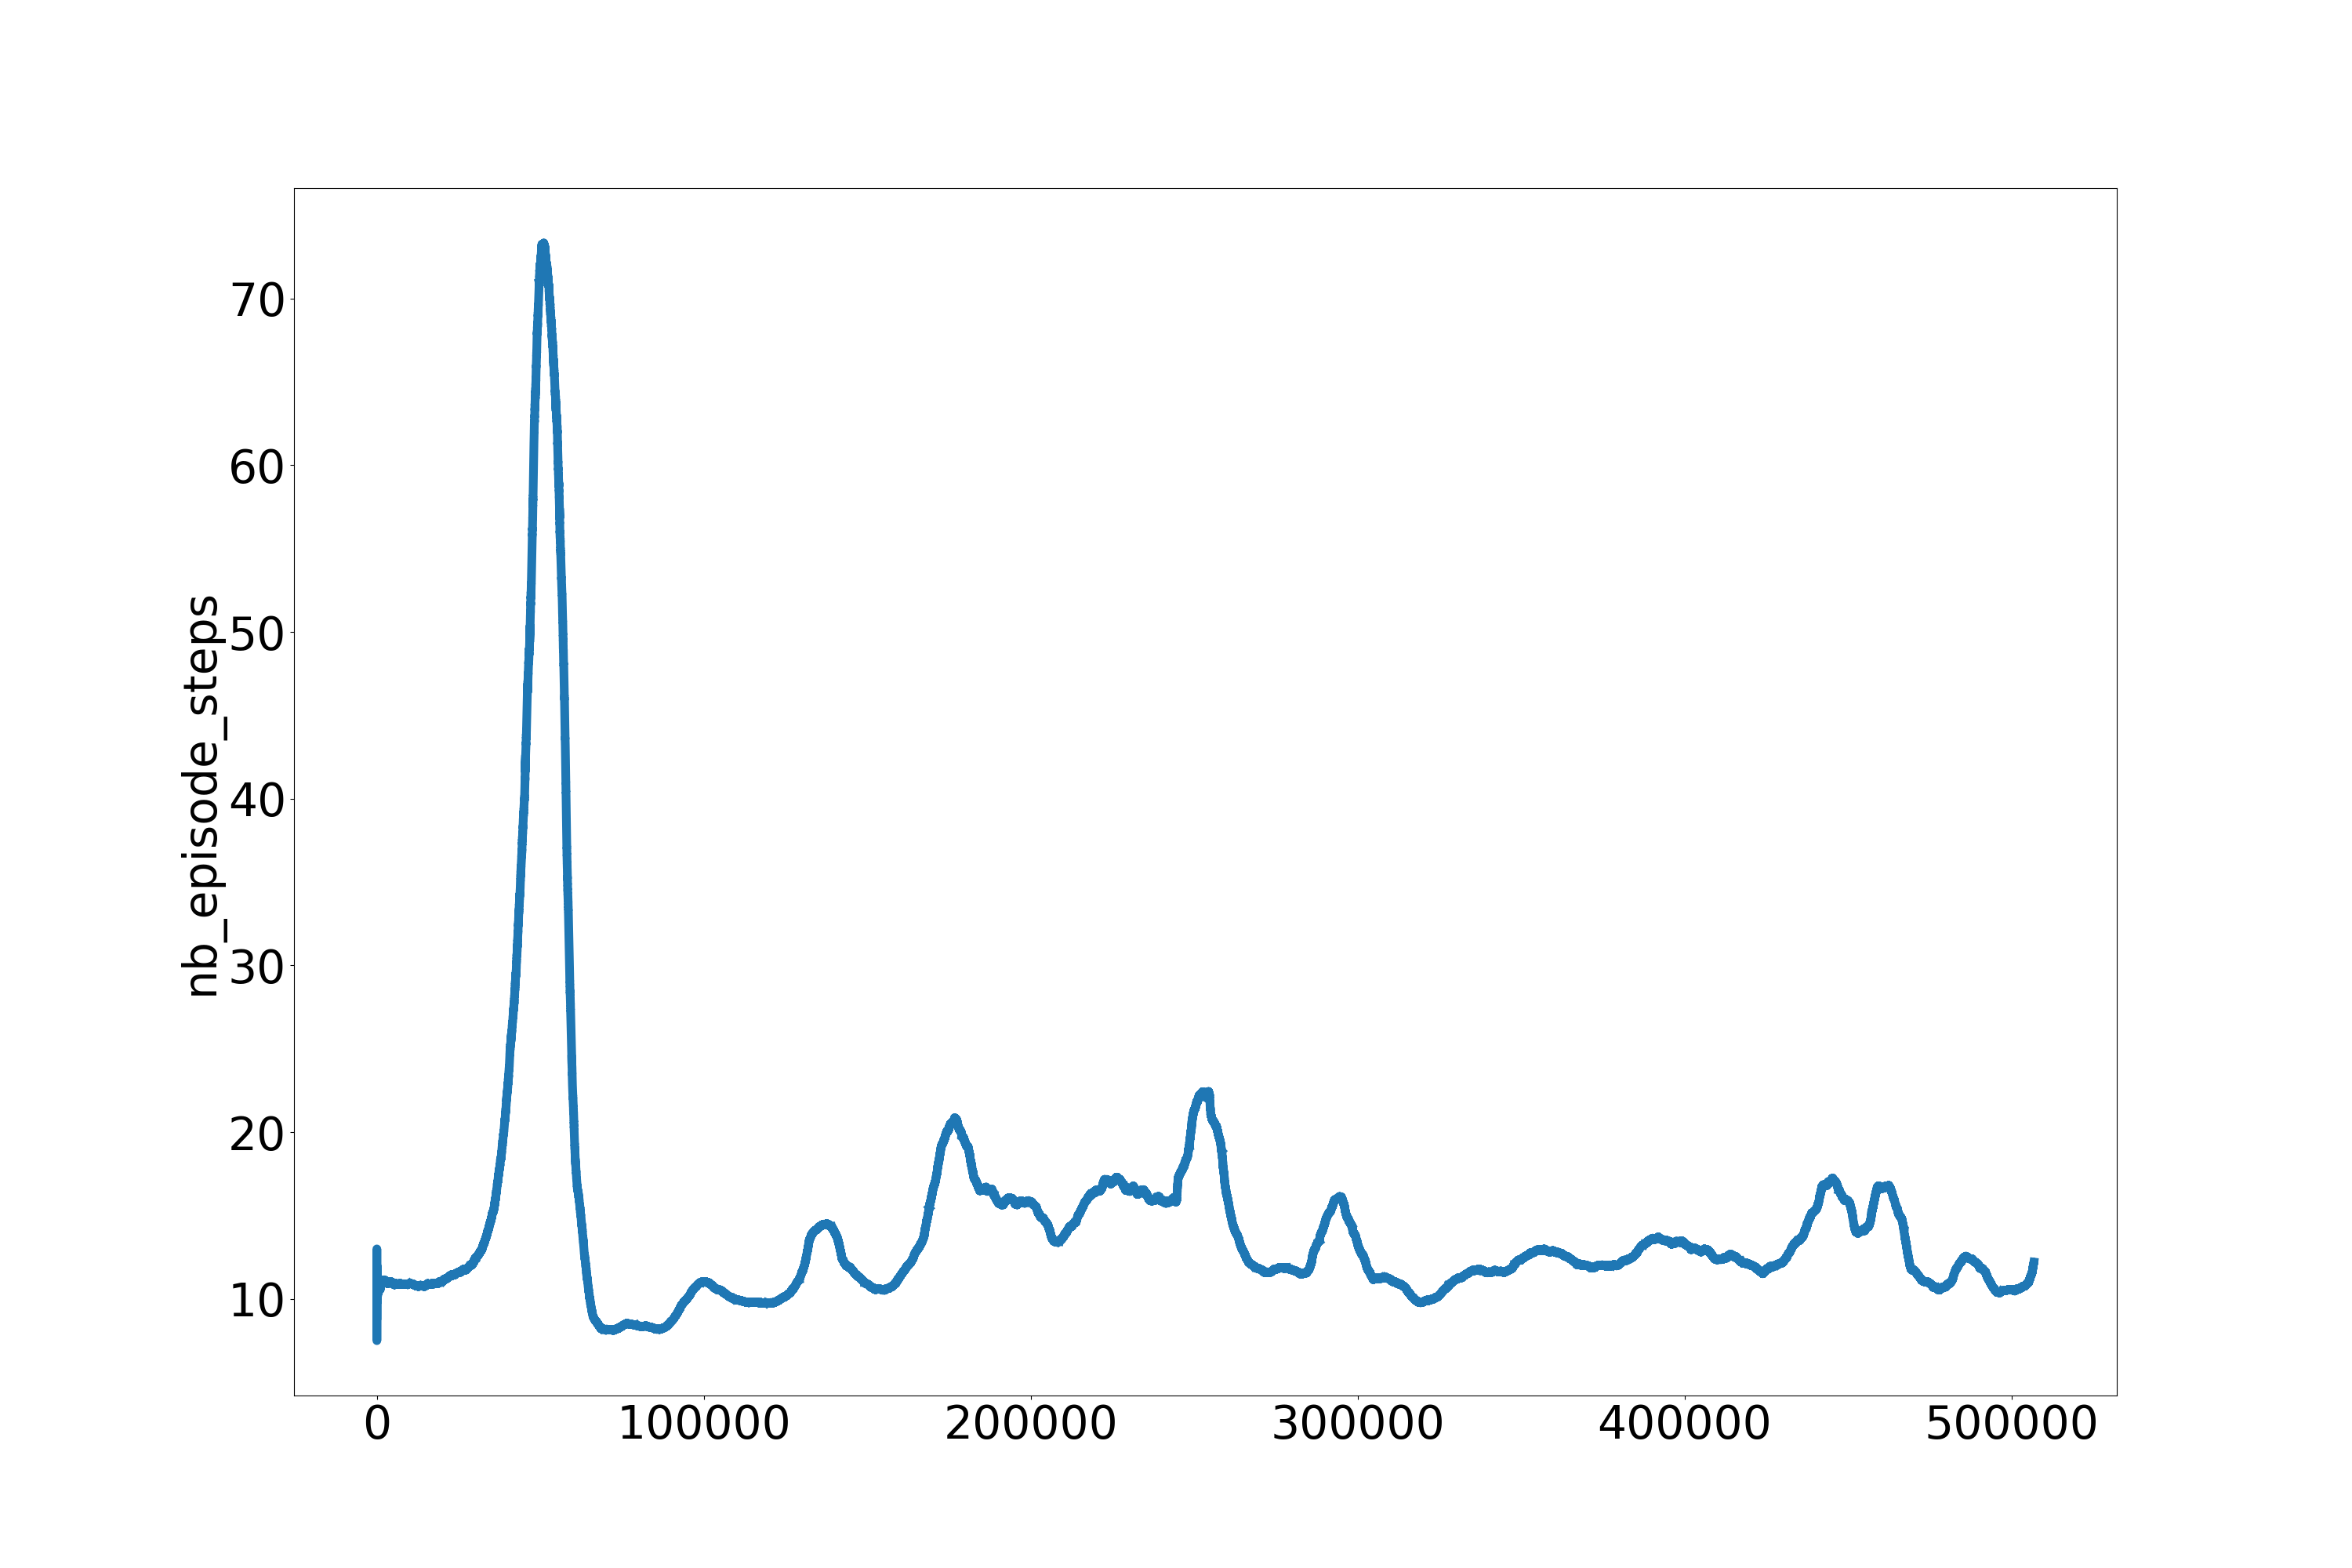
\includegraphics[width=0.85\textwidth]{Pic/Second_model/nb_episode_steps.png}
    		\caption{Số bước thực hiện}
    		\label{fig:baseline_step}
    	\end{subfigure}%
    	\begin{subfigure}{.5\textwidth}
    		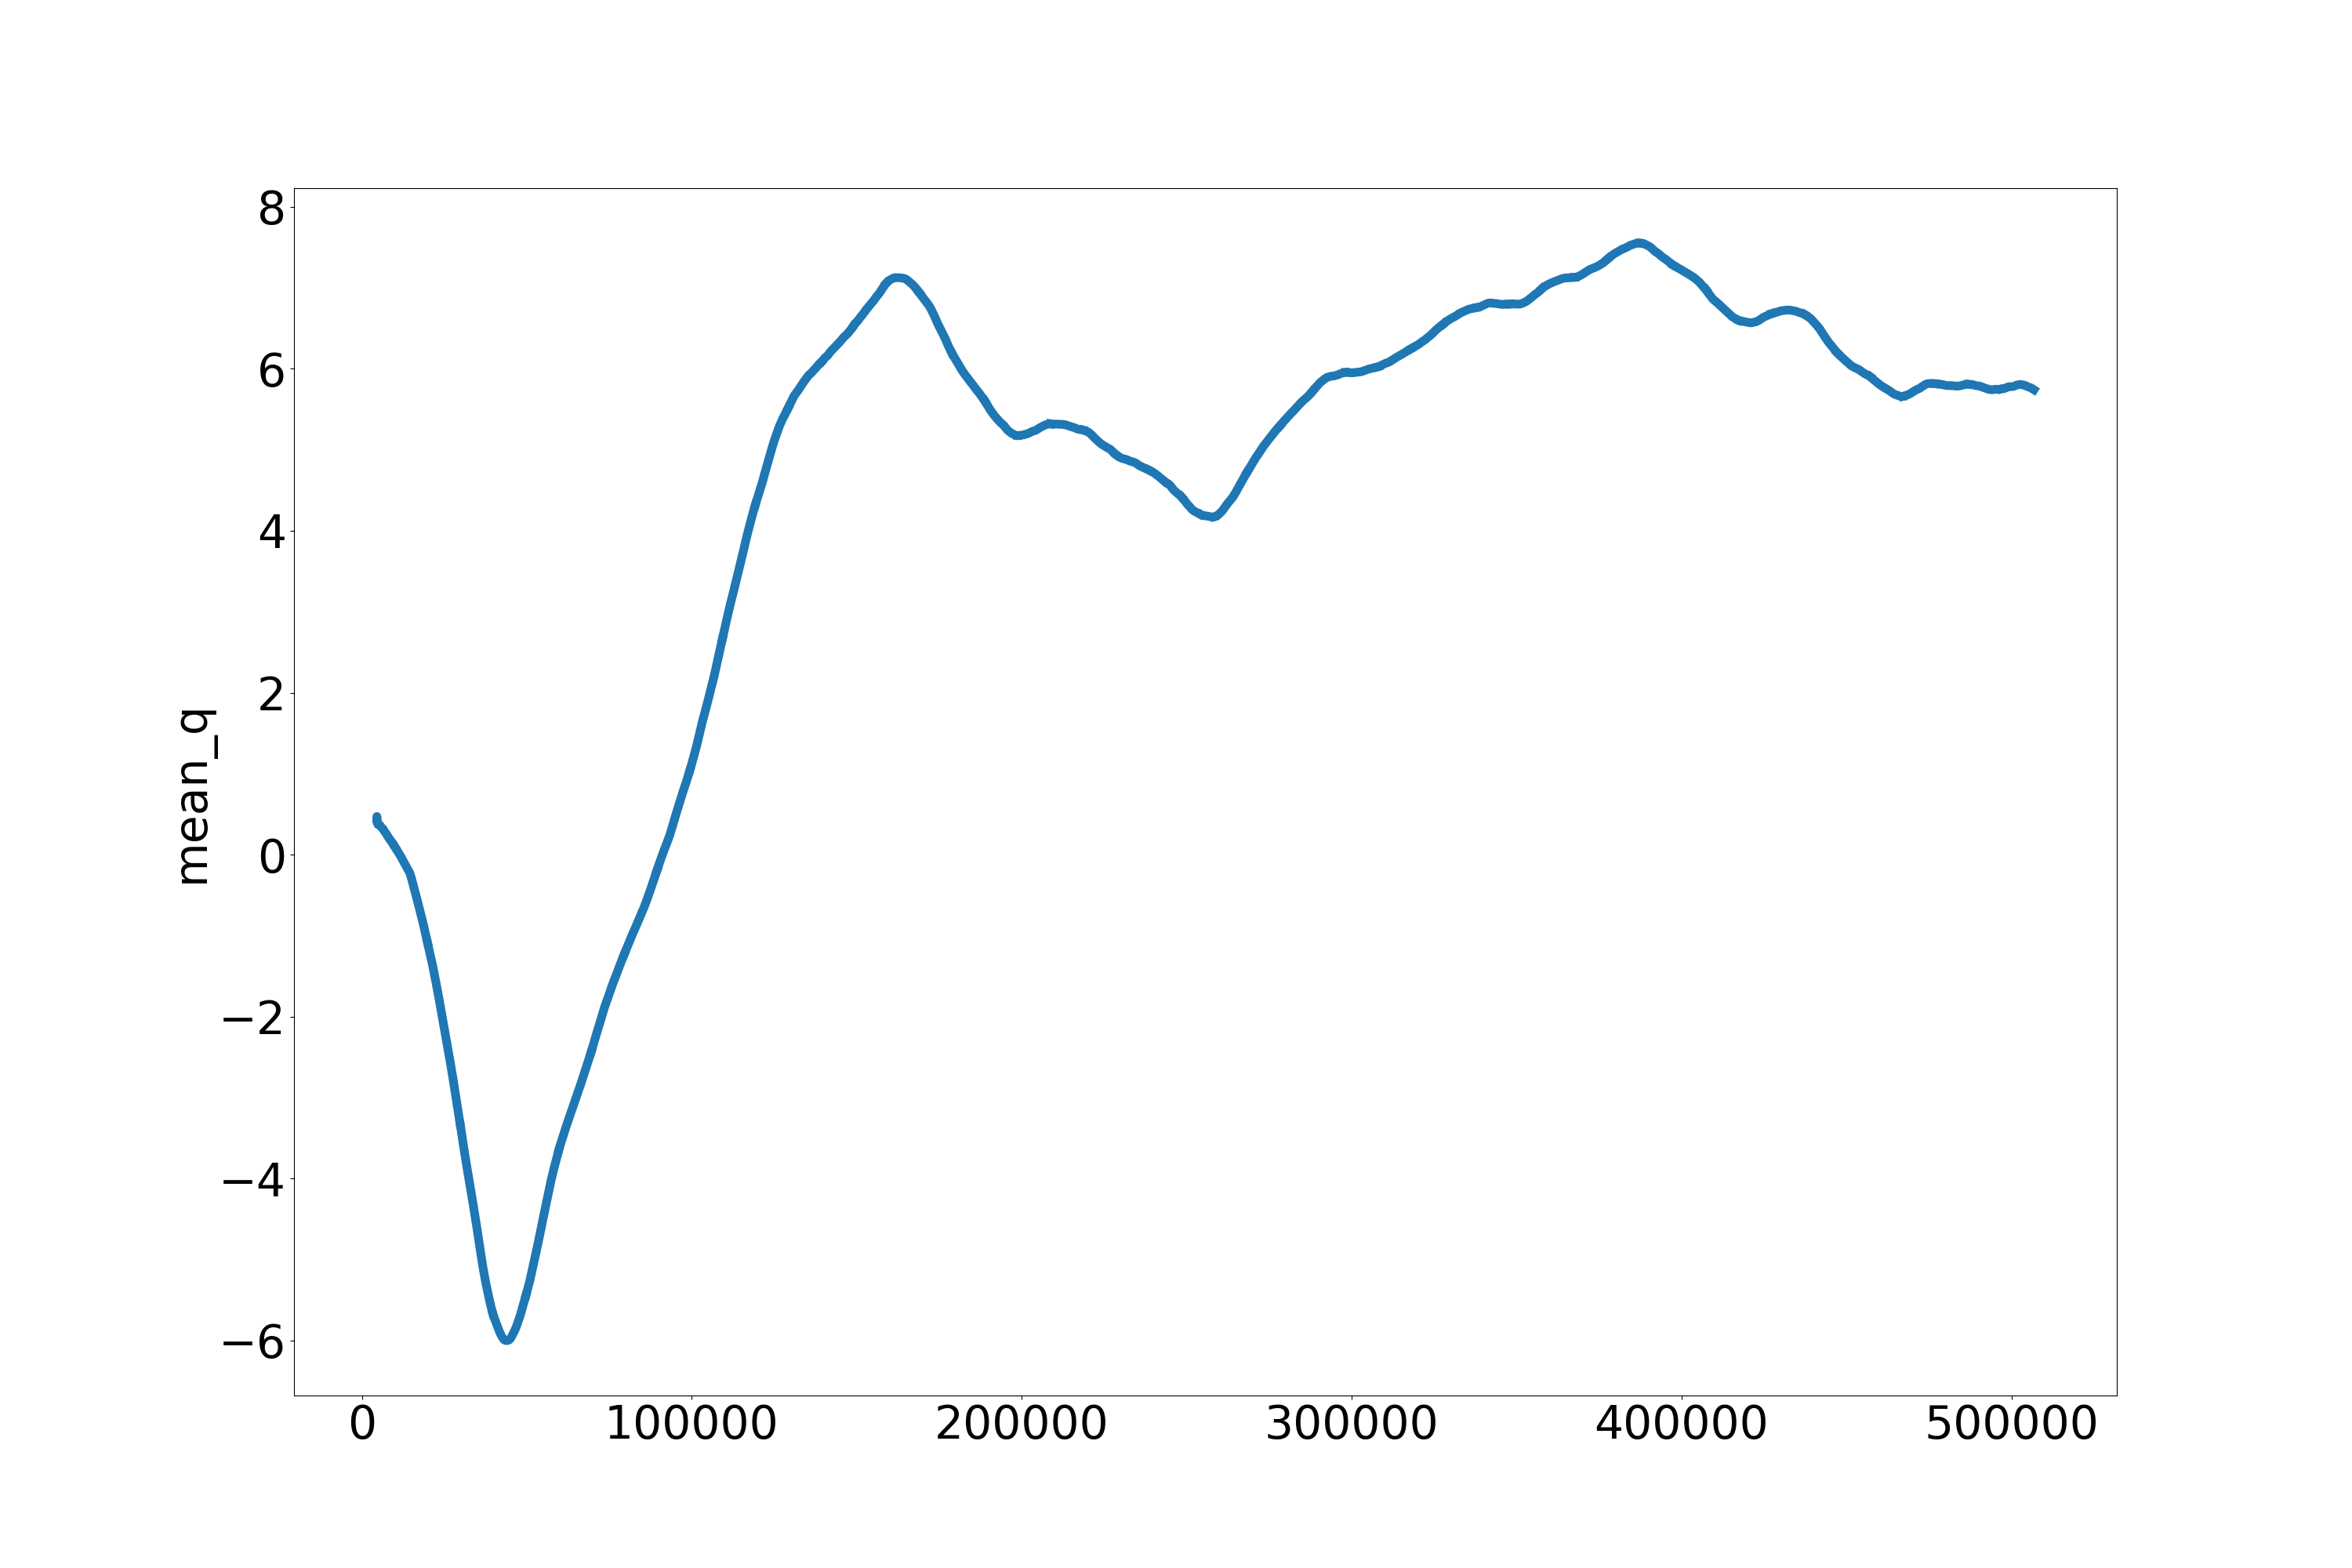
\includegraphics[width=0.85\textwidth]{Pic/Second_model/mean_q.png}
    		\caption{Trung bình giá trị Q}
    		\label{fig:baseline_mean_q}
    	\end{subfigure}
    	\label{fig:result_baseline}
    \end{figure}
\end{frame}
%%%%%%%%%%%%%%%%%%%%%%%%%%%%%%%%%%%%%%%%%%%%%%%%%%%%%%%%%%%%%%
%---------------------------------------------------------------%
\section{Kết luận}
\begin{frame}{Kết luận}
    \begin{itemize}
        \item + Các thử nghiệm hiện thời chỉ đạt tỉ lệ thắng là 55,8\%.
        \vspace{0.5cm}
        \item + Còn rất nhiều cải tiến trong tương lai.
        \vspace{0.5cm}
        \item + WHG còn nhiều vòng chơi.
    \end{itemize}
\end{frame}
%---------------------------------------------------------------%

\begin{frame}
\Huge{\centerline{The End}}
\end{frame}

%----------------------------------------------------------------------------------------

\end{document} 